\documentclass[]{book}
\usepackage{lmodern}
\usepackage{amssymb,amsmath}
\usepackage{ifxetex,ifluatex}
\usepackage{fixltx2e} % provides \textsubscript
\ifnum 0\ifxetex 1\fi\ifluatex 1\fi=0 % if pdftex
  \usepackage[T1]{fontenc}
  \usepackage[utf8]{inputenc}
\else % if luatex or xelatex
  \ifxetex
    \usepackage{mathspec}
  \else
    \usepackage{fontspec}
  \fi
  \defaultfontfeatures{Ligatures=TeX,Scale=MatchLowercase}
\fi
% use upquote if available, for straight quotes in verbatim environments
\IfFileExists{upquote.sty}{\usepackage{upquote}}{}
% use microtype if available
\IfFileExists{microtype.sty}{%
\usepackage{microtype}
\UseMicrotypeSet[protrusion]{basicmath} % disable protrusion for tt fonts
}{}
\usepackage[margin=1in]{geometry}
\usepackage{hyperref}
\PassOptionsToPackage{usenames,dvipsnames}{color} % color is loaded by hyperref
\hypersetup{unicode=true,
            pdftitle={Física da Terra},
            pdfauthor={Victor Cezar Tocantins},
            colorlinks=true,
            linkcolor=Maroon,
            citecolor=Blue,
            urlcolor=Blue,
            breaklinks=true}
\urlstyle{same}  % don't use monospace font for urls
\usepackage{natbib}
\bibliographystyle{plainnat}
\usepackage{longtable,booktabs}
\usepackage{graphicx,grffile}
\makeatletter
\def\maxwidth{\ifdim\Gin@nat@width>\linewidth\linewidth\else\Gin@nat@width\fi}
\def\maxheight{\ifdim\Gin@nat@height>\textheight\textheight\else\Gin@nat@height\fi}
\makeatother
% Scale images if necessary, so that they will not overflow the page
% margins by default, and it is still possible to overwrite the defaults
% using explicit options in \includegraphics[width, height, ...]{}
\setkeys{Gin}{width=\maxwidth,height=\maxheight,keepaspectratio}
\IfFileExists{parskip.sty}{%
\usepackage{parskip}
}{% else
\setlength{\parindent}{0pt}
\setlength{\parskip}{6pt plus 2pt minus 1pt}
}
\setlength{\emergencystretch}{3em}  % prevent overfull lines
\providecommand{\tightlist}{%
  \setlength{\itemsep}{0pt}\setlength{\parskip}{0pt}}
\setcounter{secnumdepth}{5}
% Redefines (sub)paragraphs to behave more like sections
\ifx\paragraph\undefined\else
\let\oldparagraph\paragraph
\renewcommand{\paragraph}[1]{\oldparagraph{#1}\mbox{}}
\fi
\ifx\subparagraph\undefined\else
\let\oldsubparagraph\subparagraph
\renewcommand{\subparagraph}[1]{\oldsubparagraph{#1}\mbox{}}
\fi

%%% Use protect on footnotes to avoid problems with footnotes in titles
\let\rmarkdownfootnote\footnote%
\def\footnote{\protect\rmarkdownfootnote}

%%% Change title format to be more compact
\usepackage{titling}

% Create subtitle command for use in maketitle
\providecommand{\subtitle}[1]{
  \posttitle{
    \begin{center}\large#1\end{center}
    }
}

\setlength{\droptitle}{-2em}

  \title{Física da Terra}
    \pretitle{\vspace{\droptitle}\centering\huge}
  \posttitle{\par}
  \subtitle{Notas de Aulas}
  \author{Victor Cezar Tocantins}
    \preauthor{\centering\large\emph}
  \postauthor{\par}
      \predate{\centering\large\emph}
  \postdate{\par}
    \date{28 - 05 - 2019}

\usepackage{booktabs}
\usepackage{amsthm}
\usepackage[english,brazil]{babel} % English language/hyphenation
\usepackage{microtype} % Slightly tweak font spacing for aesthetics
%\usepackage[utf8]{inputenc} % Required for including letters with accents
\usepackage[T1]{fontenc} % Use 8-bit encoding that has 256 glyphs

\usepackage{amsthm}
\newtheorem{theorem}{Teorema}[chapter]
\newtheorem{lemma}{Lema}[chapter]
\newtheorem{corollary}{Corolário}[chapter]
\newtheorem{proposition}{Preposição}[chapter]
\newtheorem{conjecture}{Conjectura}[chapter]
\theoremstyle{definition}
\newtheorem{definition}{Definição}[chapter]
\theoremstyle{definition}
\newtheorem{example}{Exemplo}[chapter]
\theoremstyle{definition}
\newtheorem{exercise}{Exercício}[chapter]
\theoremstyle{remark}
\newtheorem*{remark}{Obs}
\newtheorem*{solution}{Solução }
\let\BeginKnitrBlock\begin \let\EndKnitrBlock\end
\begin{document}
\maketitle

{
\hypersetup{linkcolor=black}
\setcounter{tocdepth}{1}
\tableofcontents
}
\hypertarget{prefacio}{%
\chapter*{Prefácio}\label{prefacio}}
\addcontentsline{toc}{chapter}{Prefácio}

Estas são as notas de aula para o curso de física da Terra, ministrados nos cursos de geologia e geofísica.

\begin{figure}
\centering
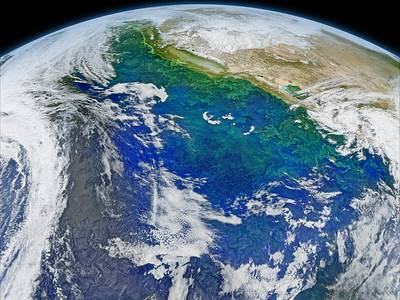
\includegraphics{images/cover.jpg}
\caption{Capa}
\end{figure}

\hypertarget{cap01}{%
\chapter{Introdução}\label{cap01}}

Neste capítulo apresentamos alguns fatos relevantes da história da geofísica, num contexto global do nosso planeta, seguimos o livro de \citet{Ribeiro2018}, onde aspectos da sismologia, gravimetria, geomagnetismo e geotermia são apresentados

\hypertarget{o-que-e-geofisica}{%
\section{O que é geofísica}\label{o-que-e-geofisica}}

A geofísica é uma das disciplinas das Ciências da Terra, ou seja, uma das ciências que se ocupam em estudar o planeta Terra - e por extensão outros corpos do Sistema Solar -, em seus diferentes aspectos.

De uma forma muito esquemática, a Terra pode ser dividida em dois ambientes muito distintos: de um lado a superfície. onde a civilização humana se desenvolveu, e a atmosfera acima dela, e de outro lado o interior do planeta. O ambiente externo é diretamente acessível à observação e, por isto, é mais bem conhecido. O conhecimento acumulado sobre a superfície da Terra e a sua atmosfera permitiu a definição de disciplinas, ou áreas de estudo, distintas entre si, mas muito integradas, como a geologia, a meteorologia, a geografia, a oceanografia e a aeronomia, também chamada de geofísica externa, porque estuda as camadas superiores da atmosfera, particularmente suas características fisioquímicas. O ambiente interno, com a exceção de uma camada muito superfícial à qual se pode ter acesso muito localizado e limitado através de grutas naturais, minas e poços profundos, só pode ser investigado por meios de métodos indiretos. Ainda assim, o conhecimento acumulado permitiu a definição de disciplinas distintas e integradas como, além da geologia, a geoquímica e a geofísica.

A geofísica, tanto externa quanta a que se ocupa do interior da Terra, é a disciplina que investiga o planeta através de métodos físicos - conforme o próprio nome indica, ainda que de forma genérica. O objetivo da geofísica é o estudo da estrutura, da dinâmica e da evolução ao longo do tempo da Terra e, desde o início da era espacial na década de 60, dos demais corpos planetários do Sistema Solar.

A grande vantagem da geofísica para a geologia, é que ela pode ser usada para fazer observações sobre a subsuperfície usando medições tomadas (geralmente) na superfície, como nos minério magnético. Na verdade, geofísica é o único ramo de as ciências da terra que podem verdadeiramente ``olhar'' para o interior da Terra, ou seja, detectar remotamente a presença de corpos e estruturas enterrados. Em contraste, geologia só pode inferi-los. Por exemplo, para as expostas dobras sinclinal da Figura \ref{fig:sinclinal}, podemos inferir vários cenários da subsuperfície, como uma falha, Figura \ref{fig:falha}, uma intrusão como ilustra a Figura \ref{fig:intrusao} ou mesmo a presença de um domo salino, Figura \ref{fig:sal}

\begin{figure}

{\centering 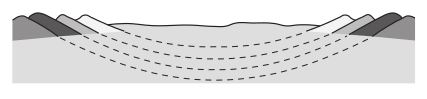
\includegraphics[width=0.7\linewidth]{fig/Fig_01.01} 

}

\caption{Sinclinal simétrica.}\label{fig:sinclinal}
\end{figure}

\begin{figure}

{\centering 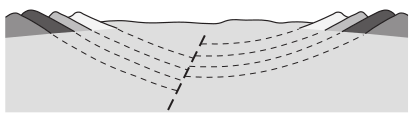
\includegraphics[width=0.7\linewidth]{fig/Fig_01.02} 

}

\caption{Sinclinal com falha.}\label{fig:falha}
\end{figure}

\begin{figure}

{\centering 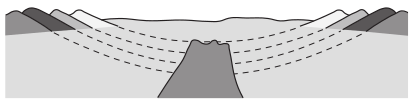
\includegraphics[width=0.7\linewidth]{fig/Fig_01.03} 

}

\caption{Sinclinal com intrusão.}\label{fig:intrusao}
\end{figure}

\begin{figure}

{\centering 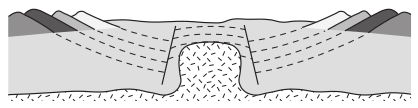
\includegraphics[width=0.7\linewidth]{fig/Fig_01.04} 

}

\caption{Sinclinal com domo de sal.}\label{fig:sal}
\end{figure}

Essas estruturas que a priori não poderiam ser inferidas apenas por amostras e estudo na superfície podem ser detectado por medições geofísicas apropriadas na superfície. Portanto, a geofísica é capaz de adicionar a terceira dimensão, profundidade, de uma forma que geologia tradicional muitas vezes não pode. Os poços podem, em princípio, fornecer informações detalhadas sobre o subsolo, mas eles são caros e, estritamente, fornecem informações apenas sobre as rochas imediatamente ao redor do furo, a estrutura da rocha distante do poço poderia ser diferente e quase sempre é devido a grande heterogeneidade da geologia. Em contraste, levantamentos geofísicos muitas vezes fornecem informações menos precisas, mas ao longo de um volume muito maior de rocha. A perfuração também é limitada em quão profundo ele pode alcançar; o furo mais profundo (Península de Kola, no noroeste da Rússia) é inferior a 13 kilometros, Figura \ref{fig:kola}, ou cerca de 1/500 da profundidade para o centro da Terra, enquanto geofísica pode sondar o todo o volume da Terra (e também explorar rochas ao redor de um poço).

Uma limitação do levantamento geofísico é que a maioria métodos dão informação apenas sobre o presente; por exemplo, não podemos registrar um terremoto que ocorreu no passado (duas notáveis exceções, são datações radiométricas para rochas e o paleomagnetismo, útil para medir movimentos de rochas ou massas de terra, mas ambos dependem em ter amostras, e não são métodos de sensoriamento remoto). Por outro lado, algumas medidas geofísicas revelam processos dinâmicos operando no Terra: Por exemplo, o estudo de terremotos informa sobre as forças que atuam dentro de zonas orogênicas.

Então, ``geofísica'', como usada neste curso, é a investigação das rochas e estruturas do subsuperfície, através de medições físicas na superfície, ou no caso de datação radiométrica e paleomagnetismo - em amostras. Pelas razões acima, a geofísica não substitui a investigação geológica, mas a complementa.

\begin{figure}

{\centering 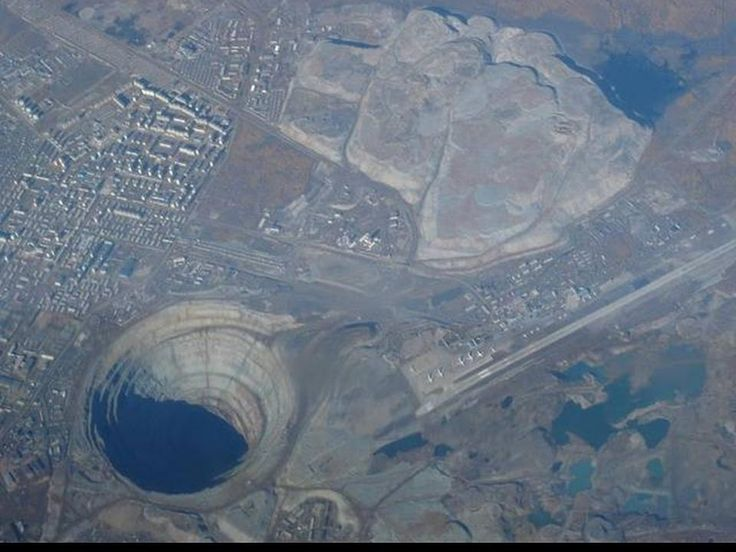
\includegraphics[width=0.7\linewidth]{fig/Fig_01.05} 

}

\caption{Super poço na penísula de Kola, na Rússia.}\label{fig:kola}
\end{figure}

\hypertarget{cap02}{%
\chapter{Gravidade, a figura da Terra e geodinâmica}\label{cap02}}

Neste capítulo seguimos o livro de \citet{lowrie_2007} apresentaremos o conceito de gravidade, anomalias gravimétricas, isostasia e reologia que são importantes tanto na geofísica global quanto na geofísica aplicada.

\hypertarget{o-tamanho-da-terra}{%
\section{O tamanho da Terra}\label{o-tamanho-da-terra}}

A primeira estimativa cientificamente sólida do tamanho do esfera terrestre foi feita por Eratóstenes (275-195 AC), que era o bibliotecário-chefe em Alexandria, uma colônia grega no Egito durante o terceiro século AC. Eratóstenes tinha dito que na cidade de Syene (moderna Assuão - Egito) raios do meio-dia do sol no dia de verão brilhou verticalmente e foram capazes de iluminar os fundos dos poços, enquanto no mesmo dia em Alexandria, sombras foram lançadas. Eratosthenes observou que no solstício de verão os raios do sol faziam um ângulo de um quinquagésimo de um círculo (\(360^\circ /50= 7.2^\circ\)) com a vertical em Alexandria, como ilustra a Figura \ref{fig:raio}

\begin{figure}

{\centering 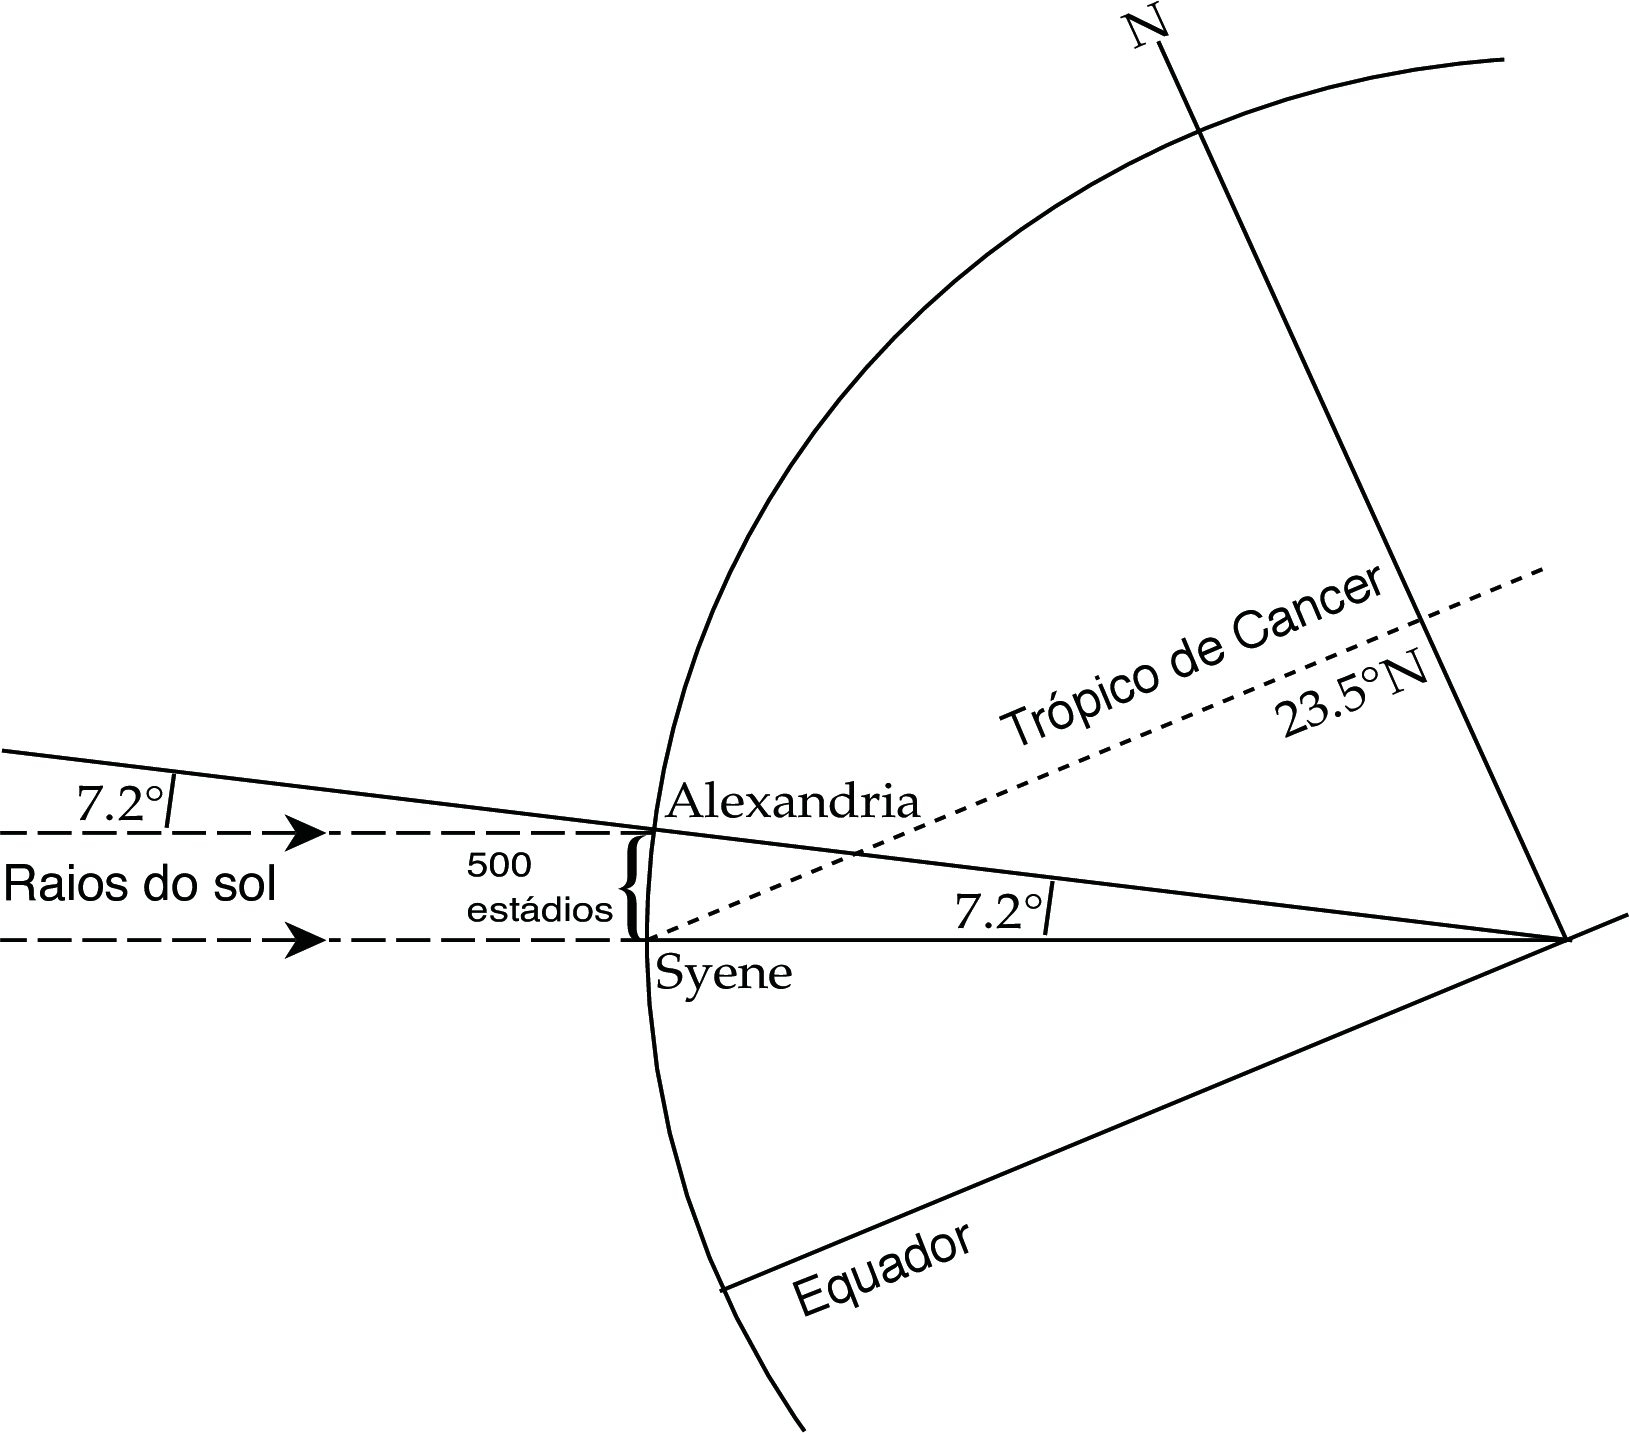
\includegraphics[width=0.4\linewidth]{fig/Fig_02.01} 

}

\caption{O método usado por Eratóstenes (275-195 AC) para estimar a circunferência da Terra usando a diferença de $7.2^\circ$ em altitude do Raios de Sol em Alexandria e Syene.}\label{fig:raio}
\end{figure}

Eratóstenes acreditava que Syene e Alexandria estavam num mesmo meridiano. Na verdade, eles estão ligeiramente deslocados; suas coordenadas geográficas são \(24^\circ\) \(5'\) N \(32^\circ\) \(56'\) E e \(31^\circ\) \(13'\) N \(29^\circ\) \(55'\) E. Syene está na verdade sobre meio grau ao norte do trópico de Câncer. Eratóstenes sabia que a distância aproximada de Alexandria para Syene foi de 5000 estádios, possivelmente estimado por viajantes do número de dias (``10 dias de camelo'') levados para viajar entre as duas cidades. A partir dessas observações Eratóstenes estimou que a circunferência do esfera global é de 250.000 estádios. O estádio grego era o comprimento (cerca de 185 m) da pista de corrida em forma de U que as corridas e outros eventos esportivos foram realizados. A Estimativa de Eratóstenes da circunferência da Terra equivale a 46.250 km, cerca de 15\% superior ao valor moderno de 40.030 km.

As estimativas do comprimento de um grau de meridiano foram feita no oitavo século DC, durante a dinastia Tang na China, e no nono século DC por astrônomos árabes na Mesopotâmia. Pouco progresso foi feito na Europa até o início do século XVII. Em 1662, a Royal Society foi fundada em Londres e em 1666 a Académie Royale des Sciences foi fundada em Paris. Ambas as organizações forneceu apoio e impulso à revolução científica. A invenção do telescópio permitiu levantamento geodésicas mais precisas. Em 1671, um astrônomo francês, Jean Picard (1620--1682), completou um levantamento preciso por triangulação do comprimento de um grau de arco meridiano. Doa seus resultados, o raio da Terra foi calculado em 6372 km, notavelmente perto do valor moderno de 6371 km.

\hypertarget{a-forma-da-terra}{%
\section{A forma da Terra}\label{a-forma-da-terra}}

Em 1672, outro astrônomo francês, Jean Richer, foi enviado por Louis XIV para fazer observações astronômicas sobre o ilha equatorial de Caiena. Ele descobriu que um pêndulo de relógio de precisão, que havia sido ajustado em Paris precisamente para bater em segundos, estava perdendo cerca de dois e meio minutos por dia, ou seja, o seu período foi agora demasiado longo. O erro foi muito grande para ser explicado pela imprecisão do instrumento. A observação despertou muito interesse e especulação, mas só foi explicado cerca de 15 anos mais tarde por Sir Isaac Newton em termos de suas leis de gravitação universal e movimento.

Newton argumentou que a forma da Terra em rotação deve ser a de um elipsoide oblato; comparado a uma esfera, deve ser um pouco achatado nos polo e protuberante para fora em torno do equador. Essa inferência foi feita em bases lógicas. Suponha que a Terra não gira e que os furos podem ser feitos para o seu centro ao longo do eixo de rotação e ao longo de um raio equatorial (Figura \ref{fig:forma}). E se esses orifícios são preenchidos com água, a pressão hidrostática no centro da Terra sustenta colunas de água iguais ao longo cada raio. No entanto, a rotação da Terra causa um força centrífuga no equador, mas não tem efeito sobre o eixo de rotação. No equador, a força centrífuga externa da rotação se opõe à atração gravitacional interna e puxa a coluna de água para fora. Ao mesmo tempo, reduz a pressão hidrostática produzida pela coluna de água no centro da Terra. A pressão central reduzida é incapaz de suportar a altura da coluna de água ao longo do raio polar, que diminui. Assim, se a Terra fosse uma esfera hidrostática, a forma da Terra em rotação deve ser um elipsoide oblato de revolução. Newton assumiu a densidade da Terra seja constante e calculado que o aplainamento deve ser de cerca de 1:230 (cerca de 0,5\%). Isso é um pouco maior do que o achatamento real da Terra, que é cerca de 1: 298 (aproximadamente 0,3\%).

\begin{figure}

{\centering 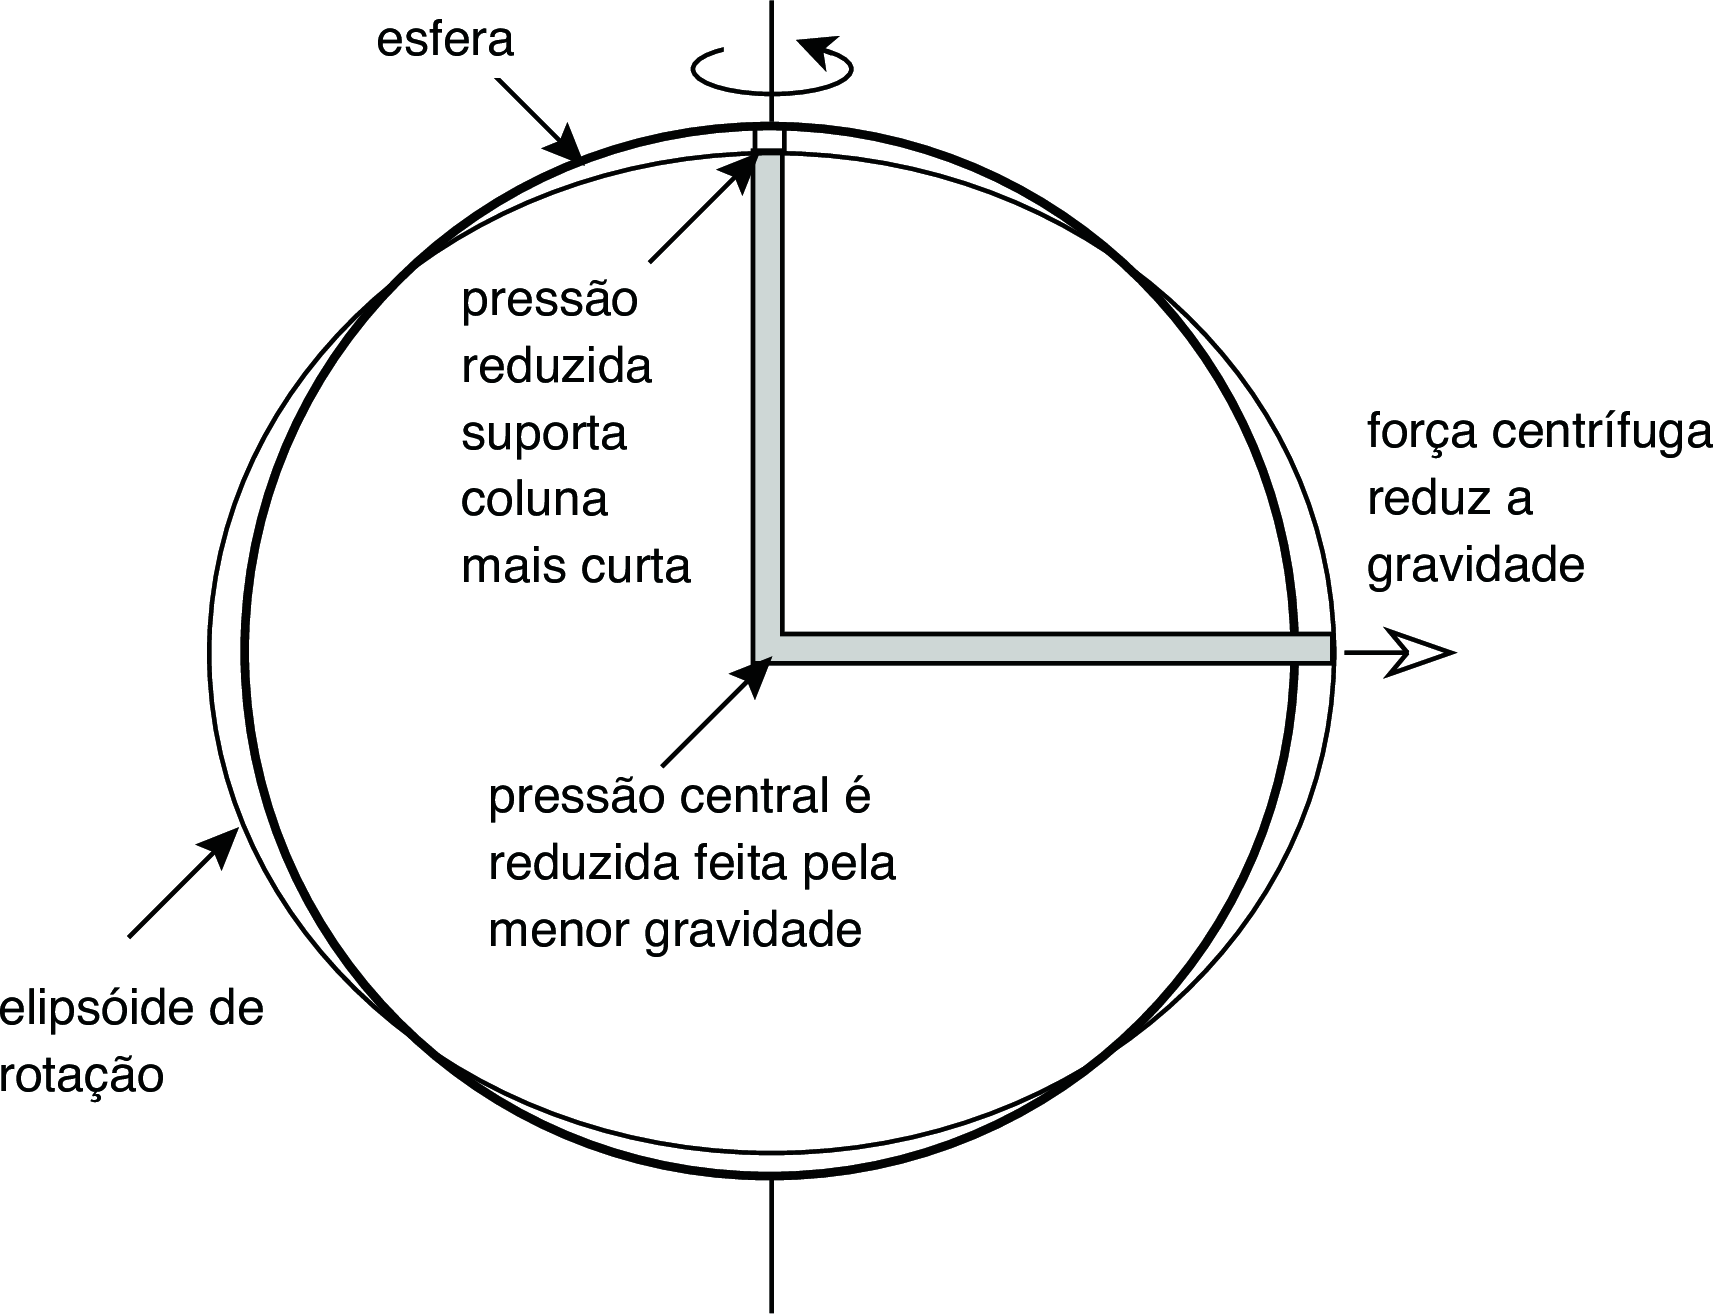
\includegraphics[width=0.4\linewidth]{fig/Fig_02.02} 

}

\caption{O argumento de Newton de que a forma da Terra em rotação deveria ser achatada nos poloss e protuberante no equador foi baseado em equilíbrio hidrostático entre colunas de pressão polar e equatorial.}\label{fig:forma}
\end{figure}

O aumento no período do pêndulo de Richer poderia agora ser explicado. Caiena estava perto do equador onde o raio maior colocou o observador mais longe do centro de atração gravitacional, e o aumento distância do eixo de rotação resultou em uma força centrífuga oposta. Esses dois efeitos resultaram em menor valor de gravidade em Caiena do que em Paris, onde o relógio havia sido calibrado.

Não houve a prova direta da interpretação de Newton. Uma corolário de sua interpretação foi que o arco do grau do meridiano deve subtender uma distância maior em regiões polares do que perto do equador (Figura \ref{fig:elipse}). No início do século XVIII profissionais em geodésia franceses estenderam a padronização do meridiano de fronteira a fronteira do país e encontrou um intrigante resultado. Em contraste com a previsão de Newton, o grau do arco meridiano diminuiu para o norte. A interpretação francesa era que a forma da Terra era um elipsoide prolato, alongada nos polos e estreitada no equador, como o forma de uma bola rugby. Uma grande controvérsia científica surgiu entre os ``niveladores'' e os ``alongadores''.

\begin{figure}

{\centering 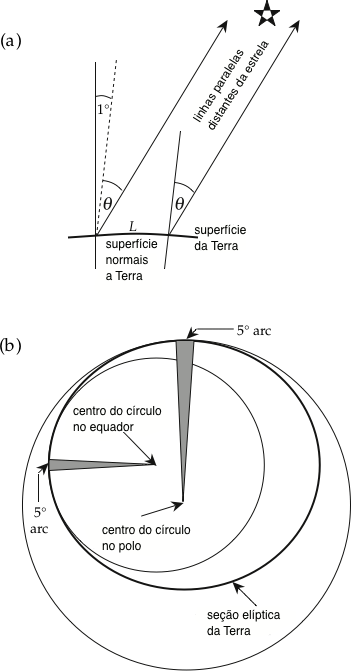
\includegraphics[width=0.4\linewidth]{fig/Fig_02.03} 

}

\caption{(a) O comprimento de um grau de arco meridiano é encontrado pela medida da distância entre dois pontos que estão a um grau de distância no mesmo meridiano. (b) O raio de curvatura maior no plano aplanado polar dá uma maior distância do arco do que é encontrado no equador onde o raio de curvatura é menor.}\label{fig:elipse}
\end{figure}

Para determinar se a forma da Terra era oblata ou prolate, a Académie Royale des Sciences patrocinou dois expedições científicas. Em 1736-1737 uma equipe de cientistas medido o comprimento de um grau de arco meridiano na Lapónia, perto do Círculo Ártico. Eles encontraram um comprimento sensivelmente mais longo que o grau de meridiano medido Picard perto de Paris. De 1735 a 1743 uma segunda parte de cientistas mediram o comprimento de mais de 3 graus de arco meridiano no Peru, perto do equador. Seus resultados mostraram que o grau de latitude equatorial era mais curto do que o grau de meridiano em Paris. Ambas as partes confirmaram convincentemente a previsão de Newton que a forma da Terra é a de um elipsoide oblato.

A forma elipsoidal da Terra resultante de sua rotação tem consequências importantes, não só para o variação com a latitude da gravidade na superfície da Terra, mas também para a taxa de rotação da Terra e a orientação do seu eixo de rotação. Estes são modificados por torques que surgem das atrações gravitacionais do Sol, Lua e planetas na forma elipsoidal.

\hypertarget{gravitacao}{%
\section{Gravitação}\label{gravitacao}}

\hypertarget{a-lei-universal-da-gravitacao}{%
\subsection{A lei universal da gravitação}\label{a-lei-universal-da-gravitacao}}

Um corpo de massa \(m\) em movimento possui um momento de inércia \((m\mathbf{v})\). Para mudarmos este movimento é necessário aplicarmos uma força \(\mathbf{F}\) a este corpo. A segunda lei de movimento de Newton estabelece que a taxa de variação do momento de uma massa é proporcional a força que atua sobre ela, e acontece na direção da força. Para o caso de massas constantes esta lei serve como definição de força \(\mathbf{F}\) em termos da aceleração \((\mathbf{a})\) dada pela massa (\(m\)):

\begin{equation}
\mathbf{F} = \frac{d}{dt} (m\mathbf{v}) = m \frac{d\mathbf{v}}{dt}= m \mathbf{a} \label{eq:0201}
\end{equation}

A unidade de força no sistema SI é o Newton (N). Ela é definida como sendo a força que dá a uma massa de um quilograma, uma aceleração de \(1\, \mathrm{m}/\mathrm{s}^2\).

Nós conhecemos a célebre observação de Newton da maçã em queda, a qual ele relacionou com a atração gravitacional que a Terra exercia sobre a maçã. Entretanto, a genialidade de Newton foi reconhecer que o campo gravitacional que faz com que a maçã caia é a mesma que mantém a Lua em órbita em torno da Terra e que mantém os planetas girando ao redor do Sol. Newton deduziu que a atração gravitacional \(\mathbf{F}\) entre duas partículas de massas \(m\) e \(M\), separadas pela distância \(r\), é proporcional ao produto destas massas e inversamente proporcional ao quadrado da distância entre elas:

\begin{equation}
\mathbf{F} = -G\frac{m M}{r^2} \hat{\mathbf{r}} \label{eq:0202}
\end{equation}

Onde \(\hat{\mathbf{r}}\) é o vetor unitário na direção da coordenada \(r\), direcionada para fora do centro de referência da massa \(M\). O sinal negativo indica que a força \(\mathbf{F}\) age na direção oposta, em direção da massa \(M\) (Figura \ref{fig:atracao}). A constante \(G\) é denominada de Constante da Gravitação Universal.

Na época de Newton não havia como determinar a constante \(G\). O método a ser seguido, seria determinar a força exercida entre duas massas no laboratório. A determinação experimental de \(G\), é extremamente difícil e foi conseguida somente depois de mais de um século após a formulação de Newton, por Lord Charles Cavendish, em 1798. Depois de uma série de medidas apuradas da força de atração entre duas esferas, Cavendish determinou o valor de \(G = 6,754 \times 10^{-11} \mathrm{m}^3 \mathrm{kg}^{-1}\mathrm{s}^{-2}\). Um valor atual da constante \(G\) é \(6,6725985 \times 10^{-11} \mathrm{m}^3 \mathrm{kg}^{-1}\mathrm{s}^{-2}\)

\begin{figure}

{\centering 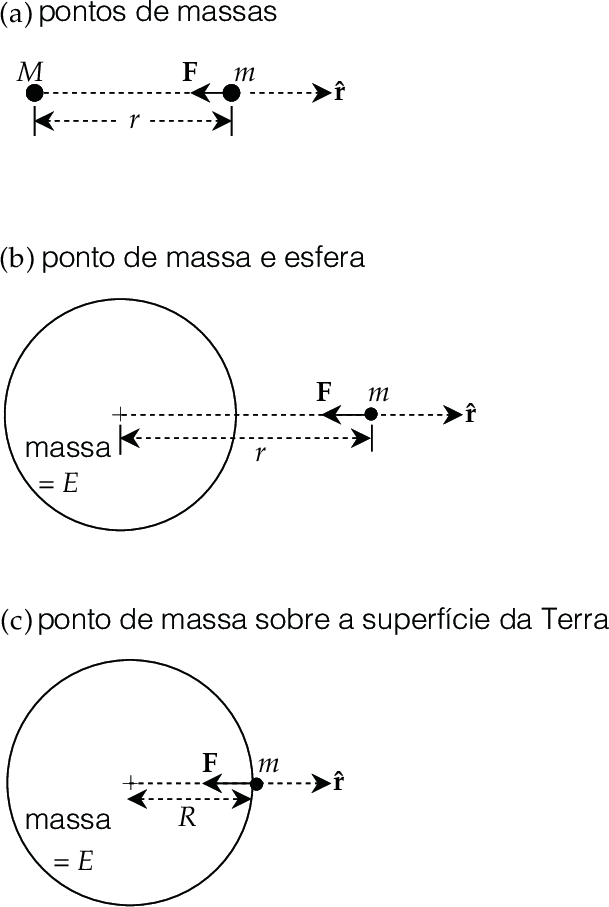
\includegraphics[width=0.4\linewidth]{fig/Fig_02.04} 

}

\caption{Geometria da atração gravitacional sobre (a) dois pontos de massa, (b) um ponto de massa fora de uma esfera, (c) um ponto de massa sobre a superfície de uma esfera.}\label{fig:atracao}
\end{figure}

\hypertarget{energia-potencial-e-trabalho}{%
\subsubsection{Energia potencial e trabalho}\label{energia-potencial-e-trabalho}}

A lei da conservação de energia significa que a energia total a em um sistema fechado é constante. Duas formas de energia devem ser consideradas aqui. A primeira é a energia potencial, em que um objeto tem em virtude de sua posição relativa a origem de uma força. A segunda é o trabalho feito contra a ação da força durante a uma variação de posição

Por exemplo, quando a maçã de Newton está na árvore, ela tem uma energia potencial mais alta do que quando está no chão. Ela cai devido à força descendente da gravidade e perde energia potencial ao fazê-lo. Para calcular a variação da energia potencial precisamos elevar a maçã à sua posição original. Isso requer que apliquemos uma força igual e oposta à atração gravitacional na maçã e, devido esta força ser movida ao longo da distância em que a maçã caiu, nós temos que gastar energia em forma de trabalho. E se a altura original da maçã acima do nível do solo era \(h\) e o valor da força exercida pela gravidade na maçã é \(F\), a força que devemos aplicar para colocá-lo de volta é \((-F)\). Assumindo que \(F\) é constante através da curta distância de sua queda, o trabalho despendido é \((-F) h\). Este é o aumento da energia potencial da maçã, quando está na árvore.

Mais geralmente, se a força constante \(F\) se move através uma pequena distância \(dr\) na mesma direção que a força, o trabalho feito é \(dW= Fdr\) e a variação na energia potencial \(dE_p\) é dada por

\begin{equation}
dE_p = -dW = -Fdr \label{eq:0203}
\end{equation}

No caso mais geral, temos que considerar os movimentos e forças que têm componentes ao longo de três ortogonal eixos. O deslocamento \(dr\) e a força \(F\) não precisam ser paralelos um ao outro. Temos que tratar \(F\) e \(dr\) como vetores. Em coordenadas cartesianas, o vetor de deslocamento \(dr\) tem componentes \((dx, dy, dz)\) e a força tem componentes \((F_x, F_y, F_z)\) ao longo de cada um dos respectivos eixos. O trabalho realizado pela componente \(x\) da força quando é deslocado ao longo do eixo \(x\) é \(F_xdx\), e existem expressões similares para os deslocamentos ao longo dos outros eixos. A variação na energia potencial \(dE_p\) é agora dada por

\begin{equation}
dE_p = -dW = -(F_xdx +F_ydy+F_zdz) \label{eq:0204}
\end{equation}

A expressão entre parênteses é chamada de produto escalar dos vetores \(\mathbf{F}\) e \(d\mathbf{r}\) definida pela expressão \(Fdr\cos{\theta}\), onde \(\theta\) é o ângulo entre os dois vetores.

\hypertarget{aceleracao-gravitacional}{%
\subsubsection{Aceleração gravitacional}\label{aceleracao-gravitacional}}

Na física, o campo de uma força é frequentemente mais importante que a magnitude absoluta da força. O campo é definido como a força exercida em uma unidade de material. Por exemplo, o campo elétrico de um corpo carregado em uma determinada posição é a força que ele exerce em uma unidade de carga elétrica naquele local. O \emph{campo gravitacional} na vizinhança de uma massa de atração é a força que exerce sobre uma massa unitária. A equação \eqref{eq:0201} mostra que isso é equivalente ao vetor de aceleração.

Em aplicações geofísicas, estamos preocupados com acelerações, e não com forças. Comparando Equação \eqref{eq:0201} e Equação \eqref{eq:0202} obtemos a aceleração gravitacional \(a_G\) da massa \(m\) devido à atração da massa \(M\)

\begin{equation}
a_G = -G\frac{M}{r^2} \hat{\mathbf{r}} \label{eq:0205}
\end{equation}

A unidade de aceleração do SI é o \((\mathrm{m}\mathrm{s}^{-2})\); esta unidade é impraticável para uso em geofísica. No agora superado sistema c.g.s. a unidade de aceleração é de \((\mathrm{cm}\,\mathrm{s}^{-2})\), que é chamado de gal em reconhecimento das contribuições de Galileo. As pequenas mudanças na aceleração da gravidade causadas pelas estruturas geológicas são medidas em milésimos desta unidade, ou seja, em miligramas (mgal). Até recentemente, anomalias de gravidade devido a estruturas geológicas foram pesquisadas com instrumentos de campo com precisão de cerca de um décimo de miligal, o que foi chamado de \emph{unidade de gravidade}. Instrumentos modernos são capazes de medir diferenças de gravidade para um milionésimo de gal, ou microgal \((\mu gal)\), que está se tornando a unidade prática de investigações de gravidade. O valor da gravidade na superfície da Terra é de cerca de \(9.8\, \mathrm{m}\mathrm{s}^{-2}\), e assim a sensibilidade das medições modernas da gravidade é de cerca de 1 parte em \(10^9\).

\hypertarget{potencial-gravitacional}{%
\subsubsection{Potencial gravitacional}\label{potencial-gravitacional}}

O potencial gravitacional é a energia potencial de uma massa unitária em um campo de atração gravitacional. Seja o potencial ser denotado pelo símbolo \(U_G\). A energia potencial \(E_p\) de uma massa \(m\) em um campo gravitacional é, portanto, igual a \((mU_G)\). Assim, uma variação na energia potencial \((dEp)\) é igual a \((m dU_G)\). A Equação \eqref{eq:0203} se torna, usando a Equação \eqref{eq:0201}

\begin{equation}
mdU_G = -Fdr = -ma_Gdr \label{eq:0206}
\end{equation}

Rearranjando esta equação conseguimos a aceleração gravitacional

\begin{equation}
a_G = -\frac{dU_G}{dr} \hat{\mathbf{r}} \label{eq:0207}
\end{equation}

Em geral, a aceleração é um vetor tridimensional. Se estivermos usando coordenadas cartesianas \((x, y, z)\), a aceleração terá componentes \((a_x, a_y, a_z)\). Estes podem ser determinados separadamente, calculando as derivadas do potencial em relação as coordenadas \(x\), \(y\) e \(z\):

\begin{equation}
a_x = -\frac{\partial U_G}{\partial x}, \quad a_y = -\frac{\partial U_G}{\partial y},\quad a_z = -\frac{\partial U_G}{\partial z} \label{eq:0208}
\end{equation}

Usando as Equações \eqref{eq:0203} e \eqref{eq:0207} temos que o potencial gravitacional de um ponto de massa \(M\):

\begin{equation}
\frac{dU_G}{dr} = G\frac{M}{r^2}
\label{eq:0209}
\end{equation}

que tem como solução

\begin{equation}
U_G = -G\frac{M}{r}.
\label{eq:0210}
\end{equation}

Para as três componentes cartesianas a equação \eqref{eq:0208} pode ser escrita como

\[a_G = -\nabla U_G \]
que é uma generalização da equação \eqref{eq:0207} onde \(\nabla\) é operador diferencial \emph{del} ou \emph{nabla} definido como

\[ \nabla=\frac{\partial}{\partial x}\hat{\mathbf{x}} + \frac{\partial}{\partial y}\hat{\mathbf{y}} + \frac{\partial}{\partial z}\hat{\mathbf{z}},\]
ou seja, a aceleração gravitacional é o negativo do gradiente do potencial.

\hypertarget{aceleracao-e-potencial-de-uma-distribuicao-de-massa}{%
\subsubsection{Aceleração e potencial de uma distribuição de massa}\label{aceleracao-e-potencial-de-uma-distribuicao-de-massa}}

Até agora, consideramos apenas a aceleração gravitacional e o potencial de massas pontuais. Um corpo sólido pode ser considerado composto de numerosas partículas pequenas, cada uma das quais exerce uma atração gravitacional em um ponto externo P (Figura \ref{fig:distribuicao}.a). Para calcular a aceleração gravitacional do objeto no ponto P, devemos formar uma soma vetorial das contribuições das partículas individuais discretas. Cada contribuição tem uma direção diferente. Supondo que \(m_i\) seja a massa da partícula na distância \(r_i\) de \(P\), isso dá uma expressão como

\begin{equation}
a_G = -G\frac{m_1}{r_1^2}\hat{\mathbf{r}}_1 -G\frac{m_2}{r_2^2}\hat{\mathbf{r}}_2 - \cdots \label{eq:0211}
\end{equation}
Dependendo da forma do sólido, esta soma vetorial pode ser bastante complicada.

Uma solução alternativa para o problema é encontra primeiro o potencial gravitacional, e então diferenciá-lo como na Equação \eqref{eq:0205} para conseguir a aceleração. A expressão para o potencial em \(P\) é

\begin{equation}
U_G = -G\frac{m_1}{r_1} -G\frac{m_2}{r_2} - \cdots \label{eq:0212}
\end{equation}

Esta é uma soma escalar, que é usualmente mais simples do que calcular uma soma vetorial.
Mais comumente, o objeto não é representado como um conjunto de partículas discretas, mas por uma distribuição de massa contínua. No entanto, podemos subdividir o volume em elementos discretos; se a densidade da matéria em cada volume é conhecida, a massa do elemento pequeno pode ser calculada e sua contribuição para o potencial no ponto externo \(P\) pode ser determinada. Ao integrar o volume do corpo, seu potencial gravitacional em \(P\) pode ser calculado. Então se considerarmos um ponto no corpo com coordenadas \((x, y, z)\) de densidade igual a \(\rho(x, y, z)\) a uma distância \(P\) igual a \(r(x,y,z)\) como na Figura \ref{fig:distribuicao}.b. O potencial gravitacional do corpo em \(P\) é:

\begin{figure}

{\centering 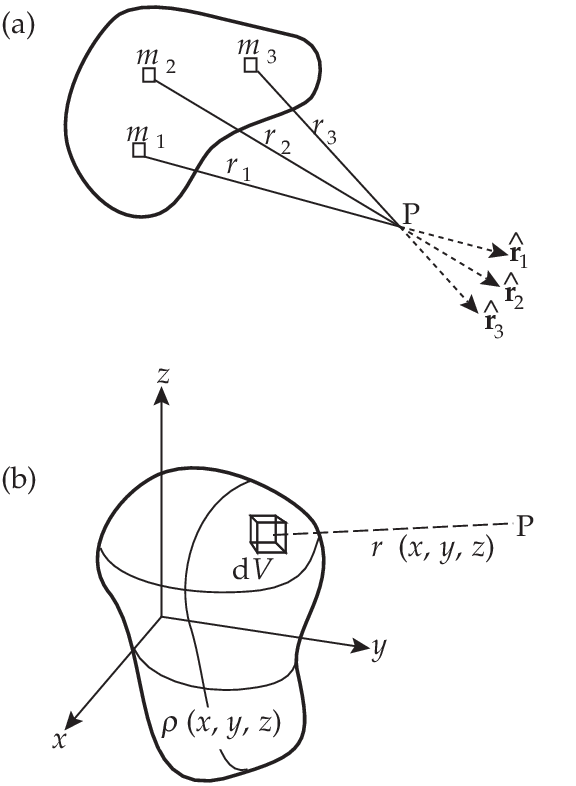
\includegraphics[width=0.4\linewidth]{fig/Fig_02.05} 

}

\caption{(a) Cada pequena partícula de um corpo sólido exerce uma atração gravitacional em uma diferente direção num ponto externo $P$, (b) Computação do potencial gravitacional de uma distribuição de massa contínua.}\label{fig:distribuicao}
\end{figure}

\begin{equation}
U_G = -G \iiint \frac{\rho(x,y,z)}{r(x,y,z)} dxdydz\label{eq:0213}
\end{equation}

A integração fornece o potencial gravitacional e a aceleração em pontos dentro e fora de uma esfera sólida oca ou homogênea. Os valores fora de uma esfera na distância \(r\) de seu centro são os mesmos como se toda a massa \(E\) da esfera estivesse concentrada em seu centro (Figura \ref{fig:atracao}.b):

\begin{equation}
U_G = -G \frac{E}{r}\label{eq:0214}
\end{equation}

\begin{equation}
\mathbf{a}_G = -G \frac{E}{r^2} \hat{\mathbf{r}}\label{eq:0215}
\end{equation}

O cálculo do potencial é muito mais simples do que o cálculo da aceleração gravitacional, como se mostra no exemplo a seguir adaptado do livro de \citet{Halliday1987}.

\BeginKnitrBlock{example}[Aceleração e potencial para uma esfera homogênea]
\protect\hypertarget{exm:unnamed-chunk-1}{}{\label{exm:unnamed-chunk-1} \iffalse (Aceleração e potencial para uma esfera homogênea) \fi{} }Considere uma casca esférica de densidade constante, cuja espessura \(t\) seja pequena em relação ao raio \(r\) (Figura \ref{fig:casca}). Desejamos calcular a aceleração gravitacional exercida numa partícula de massa \(m\) num ponto \(P\).
\EndKnitrBlock{example}

\begin{figure}

{\centering 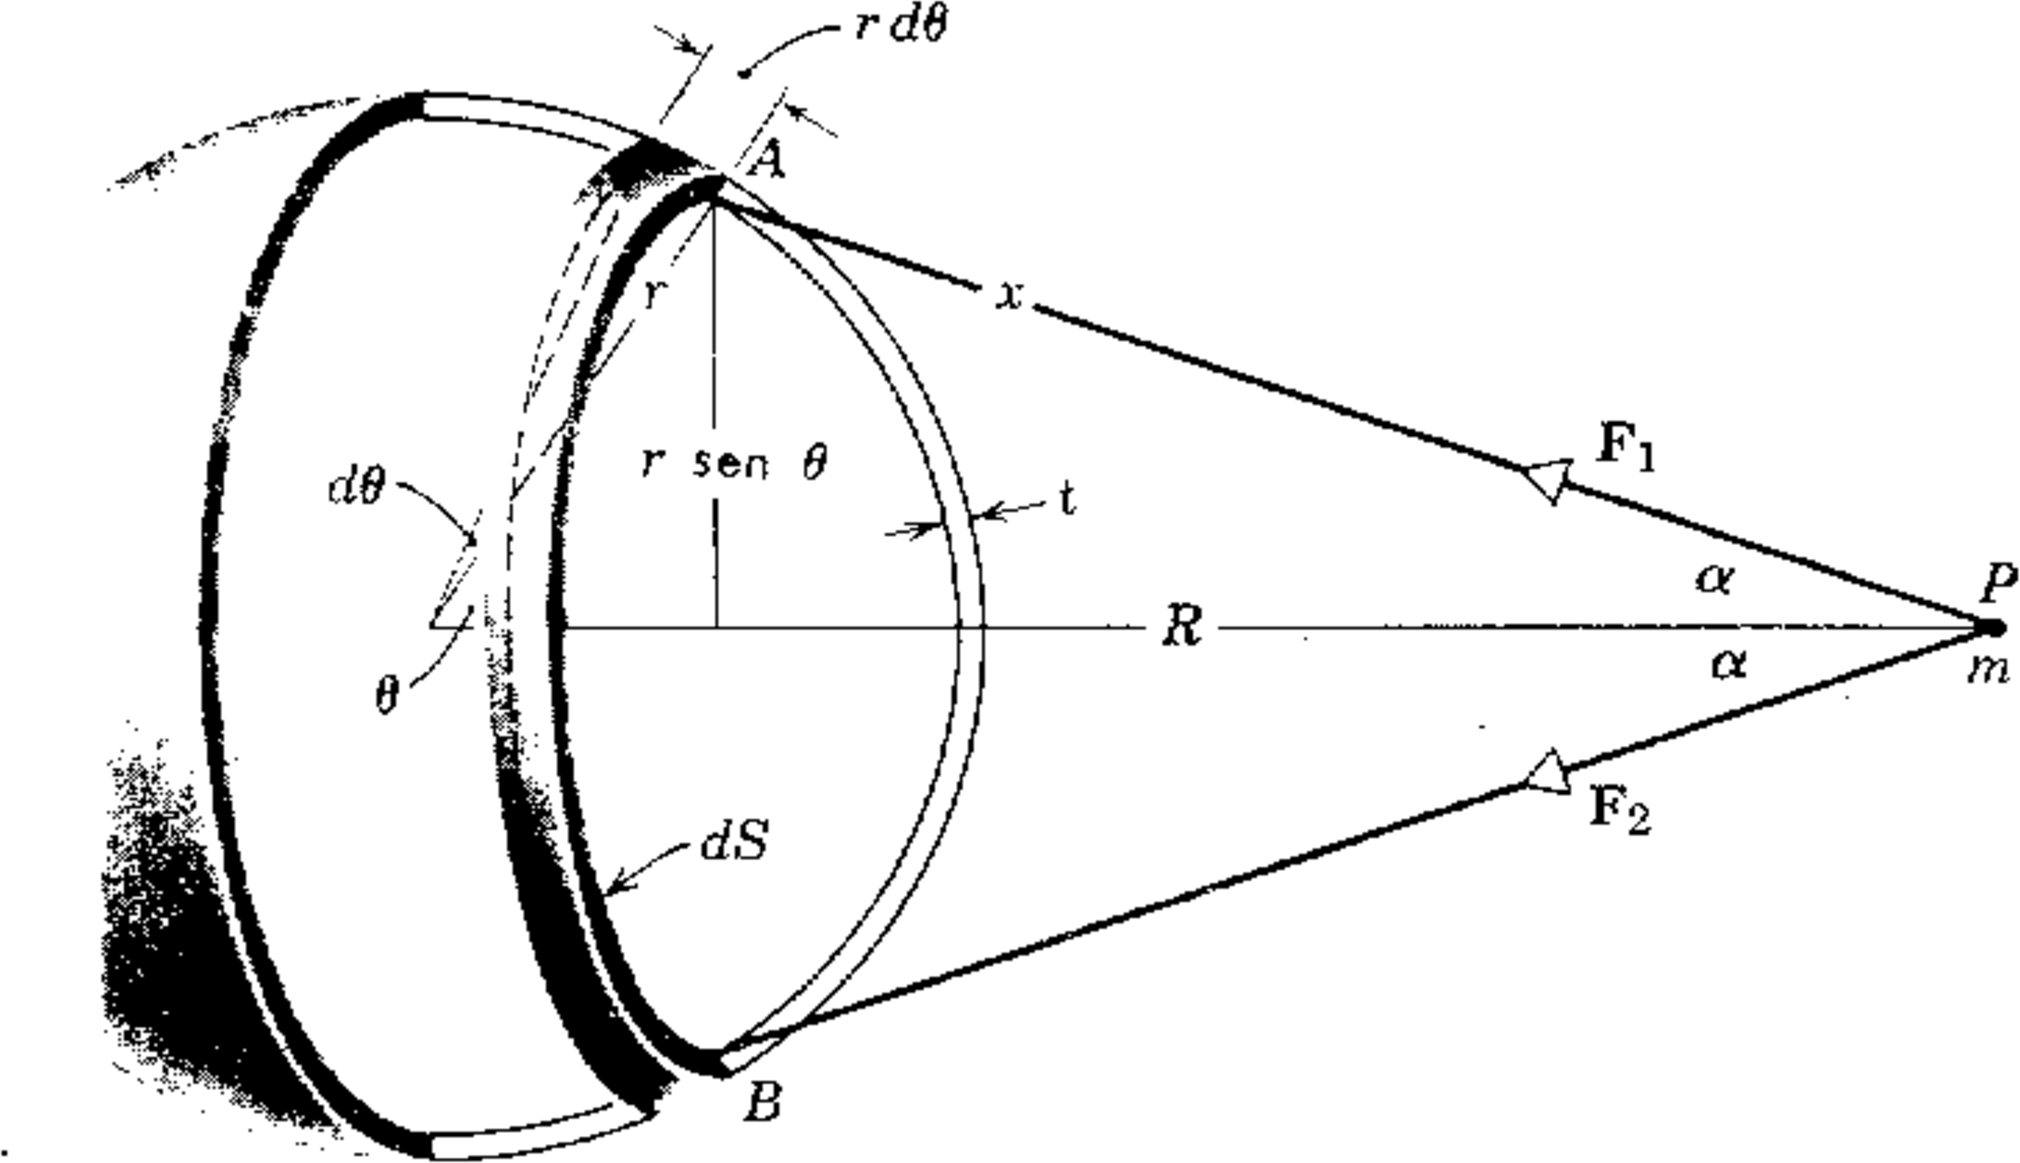
\includegraphics[width=0.6\linewidth]{fig/Fig_02.ex1} 

}

\caption{Atração gravitacional da seção $dS$ de uma casca esférica sobre uma partícula $m$.}\label{fig:casca}
\end{figure}

\textbf{Solução:}

Tomemos como elemento de massa da camada uma faixa circular de área \(dS\), com comprimento \(2\pi(r\sin{\theta})\), largura \(rd\theta\) e espessura \(t\). Seu volume será \(dV\) dado por:
\[ dV= 2\pi t r^2\sin\theta d\theta.\]
Sendo \(\rho\) a densidade da casca, sua massa será

\[ dM= \rho dV=  2\pi t \rho r^2\sin\theta d\theta.\]

Devido a simetria do problema, vemos que a aceleração exercida por \(dM\), num ponto \(A\) sobre a partícula de massa \(m\) localizada em \(P\) é horizontal tendo o valor igual
\begin{align*}
d\mathbf{a}_G &= -G\frac{dM}{x^2}\cos\alpha\; \hat{\mathbf{R}}\\
&=-2\pi G t \rho r^2\frac{\sin\theta d\theta}{x^2}\cos\alpha\; \hat{\mathbf{R}}
\end{align*}
em que \(\hat{\mathbf{R}}\) é um vetor unitário na direção da linha que une o centro da esfera \(M\) com o ponto \(P\).

As variáveis \(x\), \(\alpha\) e \(\theta\) estão relacionadas. A figura mostra que
\[ \cos\alpha = \frac{R-r\cos\theta}{x} \]
e, como, pela lei dos cossenos
\[ x^2=R^2+r^2-2Rr\cos\theta \]
tem-se

\[ r\cos\theta = \frac{R^2+r^2-x^2}{2R}\]

Assim, diferenciando a equação \(x^2=R^2+r^2-2Rr\cos\theta\), temos \(2xdx=2Rr\sin{\theta}d\theta\), ou seja

\[\sin\theta d\theta=\frac{x}{Rr}dx\]
Eliminando \(\theta\) e \(\alpha\) das equações obtemos
\[ d\mathbf{a}_G = -\frac{\pi Gt\rho r}{R^2}\left(\frac{R^2-r^2}{x^2}+1\right)\; \hat{\mathbf{R}}\]
que é aceleração exercida pela faixa circular \(dS\) sobre a partícula \(m\). Deve-se agora considerar cada elemento de massa da casca e somar todas as faixas circulares da casca: então temos uma integração sobre a casca em relação a \(x\), cujos os valores vão do mínimo \(R-r\) ao máximo \(R+r\).

Tendo em conta que
\[\int_{R-r}^{R+r}\left(\frac{R^2-r^2}{x^2}+1\right) dx =4r \]

obtêm-se a aceleração resultante

\[ \mathbf{a}_G = -\int_{R-r}^{R+r}d\mathbf{a}_G = G\frac{(4\pi r^2\rho t)}{R^2} \; \hat{\mathbf{R}}\]
Como a massa da esfera é dada por \(M=\rho V\), onde \(V\) é o volume da esfera que é igual ao produto da área de sua superfície \(4\pi r^2\) pela sua espessura \(t\), temos que \(V=4\pi r^2t\). Assim, a aceleração gravitacional é dada como:

\[ \mathbf{a}_G = -G\frac{M}{R^2}\; \hat{\mathbf{R}}\]
Por outro lado, podemos obter o mesmo valor a partir do cálculo do potencial gravitacional, uma vez que \(\mathbf{a}_G= -\nabla U_G\). Para fazer isso, conforme (\citet{fowler1990solid}), vimos que o volume circular da casca da Figura \ref{fig:casca} é dada por

\[ \rho t (2\pi r^2 \sin{\theta})(d\theta).\]

Devido cada ponto de uma faixa da casca circular ter a mesma distância \(x\) do ponto \(P\), a Equação \eqref{eq:0210} determina o potencial em \(P\) feito por essa faixa como

\[ -\frac{\rho t 2\pi r^2 \sin{\theta}d\theta}{x}\]
Novamente, aplicando a lei dos cossenos temos que \(x^2=R^2+r^2-2Rr\cos\theta.\) O potencial em toda esfera pode ser avaliado a partir da Equação \eqref{eq:0213} integrando o potencial da casca em todo o volume
\[ U_G = -G\rho t 2\pi r^2 \int_V\frac{\sin{\theta}d\theta}{(R^2+r^2-2Rr\cos\theta)^{1/2}} dV\]
Diferenciando implicitamente a expressão \(x^2=R^2+r^2-2Rr\cos\theta\) em relação a \(x\) e \(\theta\), obtemos \(xdx=Rr\sin{\theta}d\theta\), assim teremos

\[ U_G = -G\rho t 2\pi r^2 \int_V\frac{dx}{R r} dV\]
Para calcular a integral é necessário considerar dua situações: (i) quando \(P\) estiver fora da esfera \((R>r)\) e (ii), quando \(P\) está dentro da esfera \((R<r)\). Quando o ponto \(P\) é externo os limites de integração são \(R-r\) e \(R+r\) e o potencial em \(P\) é

\[ U_G = -G\rho t 2\pi r^2\left[\frac{x}{Rr}\right]_{R-r}^{R+r}=-G\frac{\rho 4\pi t r^2}{R} = -G\frac{M}{R}.\]
A aceleração gravitacional é dada por:
\[ \mathbf{a}_G = - \frac{\partial U_G}{\partial R} = -G\frac{M}{R^2}\;\hat{\mathbf{R}}\]
Quando o ponto \(P\) está dentro da esfera, o limites de integração são \(r-R\) e \(r+R\), neste caso o potencial é

\[ U_G = -G\rho t 2\pi r^2\left[\frac{x}{Rr}\right]_{r-R}^{r+R}=-G \rho 4\pi t r\]
que é constante e independe da posição \(P\) dentro da esfera. A aceleração gravitacional, sendo o negativo do gradiente do potencial, é desta forma nula dentro da esfera.

\hypertarget{massa-e-densidade-media-da-terra}{%
\subsubsection{Massa e densidade média da Terra}\label{massa-e-densidade-media-da-terra}}

As equações \eqref{eq:0214} e \eqref{eq:0215} são válidas em todos os lugares fora de uma esfera, incluindo em sua superfície onde a distância do centro de massa é igual à média do raio \(R\) (Figura \ref{fig:atracao}.c). Se considerarmos a Terra como uma primeira aproximação de uma esfera com massa \(E\) e raio \(R\), podemos estimar sua massa reescrevendo a Equação \eqref{eq:0215} como uma equação escalar na forma

\begin{equation}
E= \frac{R^2a_G}{G} \label{eq:0216}
\end{equation}

A aceleração gravitacional na superfície da Terra é apenas ligeiramente diferente da gravidade média, cerca de \(9,81\; \mathrm{m}\mathrm{s}^{-2}\), o raio da Terra é \(6371\) km, e a constante gravitacional é \(6.674\times 10^{-11}\; \text{m}^3\mathrm{kg}^{-1}\mathrm{s}^{-2}\). A massa da Terra será \(5.974\times 10^{24}\; \mathrm{kg}\). Este grande número não é tão significativo quanto sua densidade média, que pode ser calculada dividindo a massa da Terra pelo seu volume \((\tfrac{4}{3}\pi R^3)\). A densidade média de \(5515\; \mathrm{kg}\,\mathrm{m}^{-3}\), que é aproximadamente o dobro da densidade das rochas crustais. Isso indica que o interior da Terra não é homogêneo e implica que a densidade deve aumentar com a profundidade na Terra.

\hypertarget{superficies-equipotenciais}{%
\section{Superfícies equipotenciais}\label{superficies-equipotenciais}}

Uma superfície equipotencial é aquela em que o potencial é constante. Para uma esfera com determinada massa, o potencial gravitacional (Equação \eqref{eq:0215}) varia apenas com a distância \(r\) de seu centro. Um certo valor do potencial, digamos \(U_1\), é realizado a uma distância radial constante \(r_1\). Assim, a superfície equipotencial na qual o potencial tem o valor \(U_1\) é uma esfera com raio \(r_1\); uma superfície equipotencial diferente \(U_2\) é a esfera com raio \(r_2\). As superfícies equipotenciais da massa esférica original formam um conjunto de esferas concêntricas (Figura \ref{fig:potencial}.a), uma das quais (por exemplo, \(U_0\)) coincide com a superfície da massa esférica. Esta superfície equipotencial particular descreve a figura da massa esférica.

Por definição, nenhuma mudança no potencial ocorre (e nenhum trabalho é feito) em mover de um ponto para outro em uma superfície equipotencial. O trabalho feito por uma força \(F\) em um deslocamento \(dr\) é \(Fdr\cos{\theta}\) que é zero quando \(\cos{\theta}\) é zero, isto é, quando o ângulo \(\theta\) entre o deslocamento e a força é \(90^\circ\). Se nenhum trabalho é feito em um movimento ao longo de uma superfície equipotencial gravitacional, a força e aceleração do campo gravitacional devem agir perpendicular à superfície. Esta normal à superfície equipotencial define a direção \emph{vertical} ou da linha de prumo (Figura \ref{fig:potencial}.b). O plano tangencial à superfície equipotencial em um ponto define a \emph{horizontal} nesse ponto.

\begin{figure}

{\centering 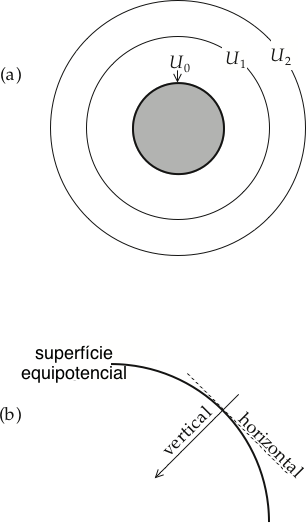
\includegraphics[width=0.4\linewidth]{fig/Fig_02.06} 

}

\caption{(a) Superfícies equipotenciais de uma massa de forma esférica forma um conjunto de esferas concêntricas, (b) A normal da superície equipotencial define a direção vertical; o plano tangente define a horizontal.}\label{fig:potencial}
\end{figure}

\hypertarget{a-figura-da-terra-e-a-gravidade}{%
\section{A figura da Terra e a gravidade}\label{a-figura-da-terra-e-a-gravidade}}

\hypertarget{a-figura-da-terra}{%
\subsection{A figura da Terra}\label{a-figura-da-terra}}

A verdadeira superfície da Terra é desigual e irregular, parcialmente terra e parcialmente água. Para fins geofísicos, a forma da Terra é representada por uma superfície lisa e fechada, chamada de figura da Terra. Os primeiros conceitos da figura eram governados por religião, superstição e crenças não científicas. A primeira circunavegação da Terra, concluída em 1522 pela equipe de Magalhães, estabeleceu que a Terra era provavelmente redonda. Antes da era do despertar científico, acreditava-se que a forma da Terra fosse uma esfera. Como confirmado por numerosas fotografias de naves espaciais, esta é de fato uma excelente primeira aproximação à forma da Terra que é adequada para resolver muitos problemas. A sugestão original de que a Terra é um esferoide achatado nos polos é creditada a Newton, que usou um argumento hidrostático para explicar o achatamento polar. A forma ligeiramente achatada permitiu uma explicação de porque um relógio de pêndulo que era preciso em Paris atrasou perto do equador.

A forma e a gravidade da Terra estão intimamente associadas. A figura da Terra é a forma de uma superfície de gravidade equipotencial, em particular aquela que coincide com o nível médio do mar. A melhor aproximação matemática da figura é um elipsoide oblato, ou esferoide (Figura \ref{fig:elipsoide}). A determinação precisa das dimensões da Terra (por exemplo, seus raios polar e equatorial) é o principal objetivo da ciência da geodésia. Ela requer um conhecimento exato do campo gravitacional da Terra, cuja descrição é o objetivo da gravimetria.

\begin{longtable}[]{@{}llll@{}}
\caption{\label{tab:parametros} Alguns parâmetros fundamentais relevantes para a forma, rotação e órbita da Terra.}\tabularnewline
\toprule
Parâmetros & Símbolo & Valores & Unidades\tabularnewline
\midrule
\endfirsthead
\toprule
Parâmetros & Símbolo & Valores & Unidades\tabularnewline
\midrule
\endhead
\emph{Parâmetros Terrestre (2004)} & & &\tabularnewline
Constante gravitacional & \(G\) & \(6.673\times 10^{-11}\) & \(\text{m}^3 \text{kg}^{-1}\text{s}^{-2}\)\tabularnewline
Constante gavitacional geocêntrica & \(GE\) & \(3.9860044\times 10^{14}\) & \(\text{m}^3 \text{s}^{-2}\)\tabularnewline
Massa da Terra: \(E=(GE)/G\) & \(E\) & \(5.9737\times 10^{24}\) & \(\text{kg}\)\tabularnewline
Raio equatorial da Terra & \(a\) & \(6378.137\) & \(\text{km}\)\tabularnewline
Raio polar da Terra: \(c=a(1-f)\) & \(c\) & \(6356.752\) & \(\text{km}\)\tabularnewline
Raio de esfera equivalente: \(R_0=(a^2c)^{1/3}\) & \(R_0\) & \(6371.000\) & \(\text{km}\)\tabularnewline
Gravidade equatorial média & \(g_e\) & \(9.7803278\) & \(\text{m}\text{s}^{-2}\)\tabularnewline
Velocidade angular média de rotação & \(\Omega\) & \(7.292115\times 10^{-5}\) & \(\text{rad}\,\text{s}^{-1}\)\tabularnewline
Fator de forma dinâmico & \(J_2\) & \(1.0826359\times 10^{-3}\) &\tabularnewline
Achatamento & \(f\) & \(1:298.252\) &\tabularnewline
Razão de aceleração equatorial & \(m\) & \(1:288.901\) &\tabularnewline
Elipticidade dinãmica & \(H\) & \(1:305.457\) &\tabularnewline
\emph{Parâmetros Orbitais (2003)} & & &\tabularnewline
Unidade astronômica & \(\text{AU}\) & \(149\,597\,870.691\) & \(\text{km}\)\tabularnewline
Razão de massa solar & \(\mu_S\) & \(332\,946.0\) &\tabularnewline
Razão de massa lunar & \(\mu_L\) & \(0.012300038\) &\tabularnewline
Obliquidade da eclíptica & \(\varepsilon_0\) & \(23^\circ\, 26'\,21.4''\) &\tabularnewline
Obliquidade da orbita lunar para eclíptica & & \(5^\circ\, 0.9'\) &\tabularnewline
Excentricidade da órbita solar do baricentro & & \(0.01671\) &\tabularnewline
Excentricidade da órbita lunar & & \(0.05490\) &\tabularnewline
\bottomrule
\end{longtable}

Análises modernas da forma da Terra são baseadas em observações precisas das órbitas dos satélites artificiais. Esses dados são usados para definir um elipsoide oblato de melhor ajuste, chamado de Elipsoide de referência internacional. Em 1930, geodesistas e geofísicos definiram um elipsoide ótimo de referência com base nos melhores dados disponíveis naquele momento. As dimensões dessa figura foram subsequentemente refinadas à medida que dados mais precisos se tornaram disponíveis. Em 1980 a Associação Internacional de Geodésia adotou um Sistema de Referência Geodésico (GRS80) no qual o elipsoide de referência tem um raio equatorial \((a)\) igual a 6378.137 km e um raio polar \((c)\) igual a 6356.752 km. As determinações subsequentes resultaram apenas em pequenas diferenças nos parâmetros geodésicos mais importantes. Alguns valores atuais estão listados na Tabela \ref{tab:parametros} apresentada no livro de \citet{lowrie_2007}. O raio da esfera equivalente \((R)\) é encontrado da fórmula \(R=(a^2 c)^{1/3}\) sendo igual a 6371.000 km. Em comparação com a esfera mais adequada, o esferóide é achatado em cerca de 14,2 km em cada polo e o equador incha em cerca de 7,1 km. O achatamento polar \(f\) é definido como a razão

\begin{figure}

{\centering 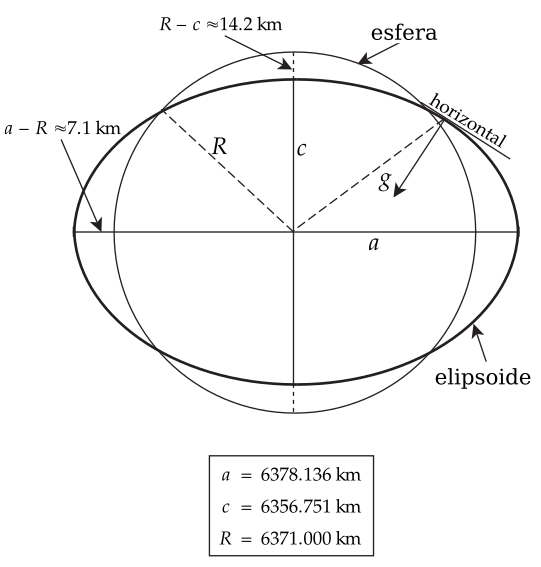
\includegraphics[width=0.4\linewidth]{fig/Fig_02.20} 

}

\caption{Comparação das dimensões do Elipsoide de referência internacional com uma esfera de igual volume.}\label{fig:elipsoide}
\end{figure}

\begin{equation}
f= \frac{a-c}{a} \label{eq:0217}
\end{equation}

O achatamento \(f\) do elipsoide de referência ótimo definido em 1930 foi exatamente 1/297. Este elipsoide e a variação da gravidade em sua superfície, serviu como base para levantamentos gravimétricos por muitos anos, até a era da geodésia por satélite e gravímetros altamente sensíveis mostrou que eram muito inexato. Uma melhor estimativa recente do achatamento é \(f=3.35287\times 10^{-3}\) (isto é, \(f=1/298.252\)).

Se assumirmos que a Terra seja um fluido rotativo em perfeito equilíbrio hidrostático (conforme assumido pela teoria de Newton), o achatamento deveria ser de \(1/299.5\), um pouco menor que o valor observado. A condição hidrostática assume que a Terra não tem força interna. Uma possível explicação para a pequena discrepância em \(f\) é que a Terra tem força suficiente para manter uma figura não hidrostática, e a figura atual é herdada de um tempo de rotação mais rápida. Alternativamente, a forma ligeiramente mais achatada da Terra pode ser devido a contrastes de densidade interna, o que poderia ser a consequência da lenta convecção no manto da Terra. Isso ocorreria em intervalos de tempo longos e poderia resultar em uma distribuição de massa não hidrostática.

A causa do achatamento polar é o efeito de deformação da aceleração centrífuga. Isso é máximo no equador, onde a aceleração gravitacional é menor. O parâmetro \(m\) é definido como a razão entre a aceleração centrífuga equatorial e a aceleração gravitacional equatorial.

\begin{equation}
m=\frac{\omega^{2}a}{GE/a^{2}}=\frac{\omega^{2}a^{3}}{GE}. \label{eq:0218}
\end{equation}

O valor de \(m\) baseado nos valores atuais da geodésia (Tabela \ref{tab:parametros}) é \(3.461\times 10^{-3}\) (i.e., \(m= 1/288.901\)). Como resultado do achatamento, a distribuição de massa dentro da Terra não depende simplesmente do raio. Os momentos de inércia da Terra em torno do eixo de rotação \((C)\) e de qualquer eixo no plano equatorial \((A)\) são desiguais. Conforme observado em \citet{lowrie_2007}, a desigualdade afeta o modo como a Terra responde aos torques gravitacionais externos e é um fator determinante nas perturbações da rotação da Terra. Os principais momentos de inércia definem a \emph{elipticidade dinâmica}:

\begin{equation}
H=\frac{C-\frac{1}{2}(A+B)}{C} \approx \frac{C-A}{C} \label{eq:0219}
\end{equation}

A elipticidade dinâmica é obtida a partir de observações precisas das órbitas dos satélites artificiais da Terra. O valor ótimo corrente para \(H\) é de \(3.2737875\times 10^{-3}\) (isto é, \(H=1/305.457\)).

\hypertarget{potencial-gravitacional-de-uma-terra-esferoidal}{%
\subsection{Potencial gravitacional de uma Terra esferoidal}\label{potencial-gravitacional-de-uma-terra-esferoidal}}

A forma elipsoidal muda o potencial gravitacional da Terra de uma esfera não deformada. Em 1849, J. MacCullagh desenvolveu a seguinte fórmula para o potencial gravitacional de qualquer corpo a grande distância de seu centro de massa:

\begin{equation}
U_{\mathrm{G}}=-G \frac{E}{r}-G \frac{(A+B+C-3 I)}{2 r^{3}}-\cdots \label{eq:0220}
\end{equation}

O primeiro termo, de ordem \(r^{-1}\), é o potencial gravitacional de um ponto de massa ou esfera com massa \(E\) (Equações \eqref{eq:0210} e \eqref{eq:0214}); para a Terra ela descreve o potencial do globo não deformado. Se os eixos de referência estão centrados no centro de massa do corpo, não há termo em \(r^{-2}\). O segundo termo, da ordem \(r^{-3}\), é devido aos desvios da forma esférica. Para a Terra aplainada ela é resultante dos deslocamentos de massa devido à deformação rotacional. Os parâmetros \(A\), \(B\) e \(C\) são os principais momentos de inércia do corpo e \(I\) é o momento de inércia em torno da linha \(OP\) que une o centro de massa ao ponto de observação (Figura \ref{fig:elipsoide2}). Para expressar o potencial com precisão, é necessário um número infinito de termos de ordem superior em \(r\). No caso da Terra, estes podem ser negligenciados, porque o próximo termo é cerca de 1000 vezes menor que o segundo termo.

\begin{figure}

{\centering 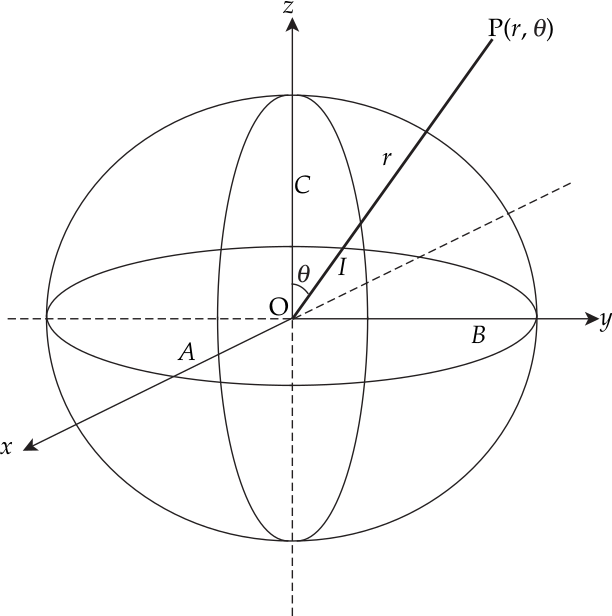
\includegraphics[width=0.4\linewidth]{fig/Fig_02.21} 

}

\caption{Parâmetros do elipsoide usado pela fórmula de MacCullagh. $A$, $B$ e $C$ são momentos de inércias em torno dos eixos $x-$, $y-$ e $z-$ respectivamente, e $I$ é o momento de inércia em torno da linha $OP$.}\label{fig:elipsoide2}
\end{figure}

Para um corpo com planos de simetria, \(I\) é uma simples combinação dos principais momentos de inércia. Configurando \(A\) igual a \(B\) para simetria rotacional, e definindo o ângulo entre \(OP\) e o eixo de rotação sendo \(\theta\), a expressão para \(I\) é

\begin{equation}
I=A \sin ^{2} \theta+C \cos ^{2} \theta \label{eq:0221}
\end{equation}

A fórmula de MacCullagh para a Terra elipsoidal então torna-se

\begin{equation}
U_{\mathrm{G}}=-G \frac{E}{r}+G \frac{(C-A)\left(3 \cos ^{2} \theta - 1\right)}{2 r^{3}} \label{eq:0222}
\end{equation}

A função \(\left(3 \cos ^{2} \theta - 1\right) / 2\) é um polinômio de segunda ordem em \(\cos\theta\), e escrevemos como \(P_2(\cos\theta)\). Ele pertence a uma família de funções chamadas de polinômios de Legendre. Usando esta notação a fórmula de MacCullagh para o potencial gravitacional do elipsoide oblato torna-se

\begin{equation}
U_{G}=-G \frac{E}{r}+G \frac{(C-A)}{r^{3}} P_{2}(\cos \theta)  \label{eq:0223}
\end{equation}

Esta pode ser escrita na forma alternativa

\begin{equation}
U_{\mathrm{G}}=-G \frac{E}{r}\left(1-\left(\frac{C-A}{E R^{2}}\right)\left(\frac{R}{r}\right)^{2} P_{2}(\cos \theta)\right) \label{eq:0224}
\end{equation}

A Equação \eqref{eq:0224} é uma aproximação para o potencial de um elipsoide. Para uma maior precisão precisamos de uma matemática um pouco mais avançada, é o que veremos a seguir.

A teoria do potencial requer que o potencial gravitacional da Terra esferoidal deva satisfazer uma importante equação, a equação de Laplace: \(\nabla^2U_\mathrm{G}\). A solução dessa equação é a soma de um número infinito de termos de ordem crescente em \(1/r\), cada um envolvendo um polinômio de Legendre apropriado e ela é dada por:

\begin{equation}
U_{\mathrm{G}}=-G \frac{E}{r}\left(1-\sum_{n=2}^{\infty}\left(\frac{R}{r}\right)^{n} J_{n} P_{n}(\cos \theta)\right)
\label{eq:0225}
\end{equation}

Nesta equação, os coeficientes \(J_n\) multiplicando \(P_n(\cos\theta)\) determinam a importância relativa do termo de enésima ordem. Os valores de \(J_n\) são obtidos a partir da geodésia do satélite: \(J_2= 1082.6\times 10^{-6}\); \(J_3= -2.54\times 10^{-6}\); \(J_4=-1.59\times 10^{-6}\); ordens mais altas são insignificantes. O coeficiente mais importante é o de segunda ordem, o fator forma dinâmica \(J_2\), que descreve o efeito do achatamento polar no potencial gravitacional da Terra. Uma comparação dos termos das Equações. \eqref{eq:0224} e \eqref{eq:0225} dá o resultado

\begin{equation}
J_{2}=\frac{C-A}{E R^{2}} \label{eq:0226}
\end{equation}

O termo de próxima ordem superior \((n=3)\) na Equação \eqref{eq:0225} descreve os desvios do elipsoide de referência que correspondem a uma Terra em forma de pera (Figura \ref{fig:elipsoide3}). Estes desvios são da ordem de \(7-17\) m, mil vezes menores que os desvios do elipsoide de um esfera, que são da ordem de \(7-14\) km.

\begin{figure}

{\centering 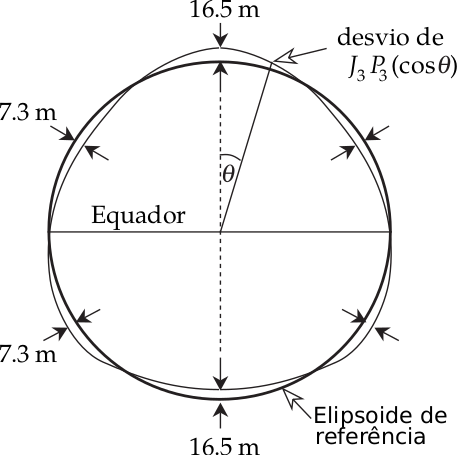
\includegraphics[width=0.4\linewidth]{fig/Fig_02.22} 

}

\caption{O termo de terceira ordem no potencial gravitacional descreve uma Terra em forma de pera. Os desvios do elipsoide de referência são da ordem de $10$ a $20$ m, muito menores que os desvios do elipsoide de uma esfera, que são da ordem de 4104 a $20$ km.}\label{fig:elipsoide3}
\end{figure}

\hypertarget{o-potencial-centrifugo}{%
\subsection{O potencial centrífugo}\label{o-potencial-centrifugo}}

A aceleração centrífuga é o gradiente do potencial centrífugo \(U_\mathrm{c}\),

\begin{equation*}
\mathbf{a}_{\mathrm{c}}=-\nabla U_{\mathrm{c}}
\end{equation*}

Seja \(x\) a distância perpendicular do eixo de rotação a um ponto na superfície na latitude \(\theta\) e seja \(\omega\) a taxa angular de rotação da Terra (Figura \ref{fig:centrifugo}). A aceleração centrífuga é igual a \(\omega^2 x\), portanto, para uma taxa constante de rotação, \(U_\mathrm{c}\) varia apenas com \(x\). Assim sendo

\begin{equation*}
\omega^{2} x=-\frac{\partial U_{\mathrm{c}}}{\partial x}
\end{equation*}

\begin{figure}

{\centering 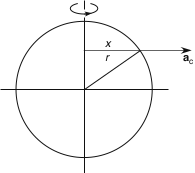
\includegraphics[width=0.4\linewidth]{fig/Fig_02.23} 

}

\caption{Aceleração centrífuga $\mathbf{a}_\mathrm{c}$ em co-latitude $\theta$ direcionada perpendicularmente para fora do eixo de rotação.}\label{fig:centrifugo}
\end{figure}

integrando ambos os lados em relação a \(x\) teremos

\begin{equation*}
U_{\mathrm{c}}=-\frac{1}{2} \omega^{2} x^{2}+U_{0}
\end{equation*}

O potencial é zero no eixo de rotação, onde \(x = 0\) e a constante de integração \(U_\mathrm{c} = 0\). A equação para o potencial centrífugo em termos de ângulo polar \(\theta\) é

\begin{equation*}
U_{\mathrm{c}}=-\frac{1}{2} \omega^{2} x^{2}=-\frac{1}{2} \omega^{2} r^{2} \sin ^{2} \theta
\end{equation*}

\hypertarget{gravidade-e-seu-potencial}{%
\subsection{Gravidade e seu potencial}\label{gravidade-e-seu-potencial}}

O potencial de gravidade \((U_\mathrm{g})\) é a soma dos potenciais gravitacional e centrífugo. É frequentemente chamado de geopotencial. Em um ponto na superfície do esferóide rotativo, ele pode ser escrito

\begin{equation}
U_{\mathrm{g}}=U_{\mathrm{G}}-\frac{1}{2} \omega^{2} r^{2} \sin ^{2} \theta \label{eq:0227}
\end{equation}

Se a superfície livre é uma superfície de gravidade equipotencial, então \(U_\mathrm{g}\) é constante em toda superfície. A forma da superfície equipotencial é restrita a ser a do esferoide com aplanamento \(f\). Nestas condições, uma relação simples é encontrada entre as constantes \(f\), \(m\) e \(J_2\):

\begin{equation}
J_{2}=\frac{1}{3}(2 f-m) \label{eq:0228}
\end{equation}

Pelas Equações \eqref{eq:0226} e \eqref{eq:0228} e reordenando os termos obtemos a seguinte relação

\begin{equation}
\frac{C-A}{E R^{2}}=\frac{1}{3}(2 f-m) \label{eq:0229}
\end{equation}

Isso produz informações úteis sobre a variação de densidade dentro da Terra. As quantidades \(f\), \(m\) e \((C-A)/C\) são iguais a aproximadamente \(1/300\). Inserir seus valores na equação fornece \(C \approx 0.33ER^2\). Compare este valor com os principais momentos de inércia de um casco esférico oco \((0.66ER^2)\) e uma esfera sólida com densidade uniforme \((0.4ER^2)\). A concentração de massa perto do centro causa uma redução no fator de multiplicação de \(0.66\) para \(0.4\). O valor de \(0.33\) para a Terra implica que, em comparação com uma esfera sólida uniforme, a densidade deve aumentar em direção ao centro da Terra.

\hypertarget{a-gravidade-normal}{%
\subsection{A gravidade normal}\label{a-gravidade-normal}}

A direção da gravidade em um ponto é definida como perpendicular à superfície equipotencial através do ponto. Isso define a \emph{vertical} no ponto, enquanto o plano tangencial à superfície equipotencial define a \emph{horizontal} (Figura \ref{fig:elipsoide}). Uma consequência da forma esferoidal da Terra é que a direção vertical geralmente não é radial, exceto no equador e nos polos.

Em uma Terra esférica, não há ambiguidade na forma como definimos a latitude. É o ângulo no centro da Terra entre o raio e o equador, o complemento ao ângulo polar \(\theta\). Isso define a latitude geocêntrica \(\lambda'\). No entanto, a latitude geográfica em uso comum não é definida dessa maneira. É encontrado pela medição geodésica do ângulo de elevação de uma estrela fixa acima do horizonte. Mas o plano horizontal é tangencial ao elipsoide, não a uma esfera (Figura \ref{fig:elipsoide}), e a direção vertical (isto é, a direção local da gravidade) intercepta o equador em um ângulo \(\lambda'\) que é ligeiramente maior que a latitude geocêntrica \(\lambda'\) (Figura \ref{fig:elipsoide4}). A diferença \((\lambda-\lambda')\) é zero no equador e nos polos e atinge um máximo numa latitude de \(45^\circ\) onde é apenas \(0.19^\circ\) (em torno de \(12'\))

O \emph{elipsoide de Referência Internacional} é a referência padronizada da figura da Terra. O valor teórico da gravidade no elipsoide rotativo pode ser calculada diferenciando o potencial de gravidade (Equação \eqref{eq:0227}). Este produz os componentes radiais e transversais da gravidade, que são então combinados para dar a seguinte fórmula para a gravidade normal ao elipsoide:

\begin{equation}
g_{\mathrm{n}}=g_{\mathrm{e}}\left(1+\beta_{1} \sin ^{2} \lambda+\beta_{2} \sin ^{2} 2 \lambda\right) \label{eq:0230}
\end{equation}

onde, para a segunda ordem em \(f\) e \(m\),

\begin{align}
g_{\mathrm{n}}&=g_{\mathrm{e}}\left(1+f-\frac{3}{2} m+f^{2}-\frac{27}{14} f \mathrm{m}\right) \nonumber \\
\beta_{1} &=\frac{5}{2} m-f+\frac{15}{4} m^{2}-\frac{17}{14} \mathrm{fm} \label{eq:0231}\\
\beta_{2} &=\frac{1}{8} f^{2}-\frac{5}{8} \mathrm{fm} \nonumber
\end{align}

\begin{figure}

{\centering 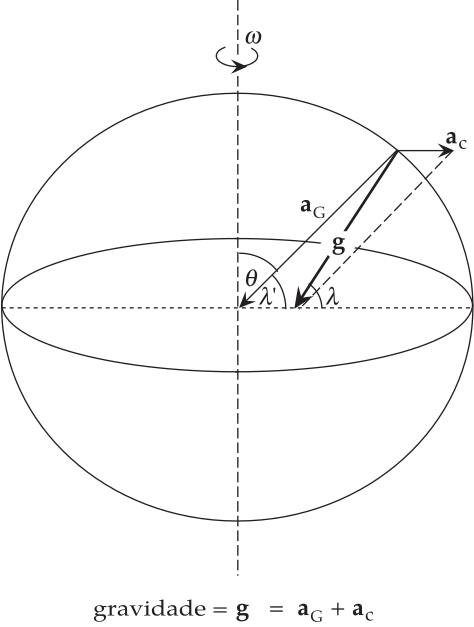
\includegraphics[width=0.4\linewidth]{fig/Fig_02.24} 

}

\caption{A gravidade na terra elipsoidal é a soma vetorial das acelerações gravitacional e centrífuga e não é radial; consequentemente, a latitude geográfica ($\lambda$) ligeiramente maior que geocêntrica latitude ($\lambda'$). }\label{fig:elipsoide4}
\end{figure}

A Equação \eqref{eq:0230} é conhecida como a fórmula de gravidade normal. As constantes na fórmula, definidas em 1980 para o \emph{Sistema de Referência Geodésico (GRS80)} ainda em uso comum, são: \(g_e= 9.780327\, \text{m}\text{s}^{-2}\); \(\beta_1=5.30244\times 10^{-3}\); \(\beta_2 = -5.8\times 10^{-6}\). Eles permitem o cálculo da gravidade normal em qualquer latitude com uma precisão de \(0.1\) mgal. Instrumentos modernos podem medir diferenças de gravidade com precisão ainda maior, neste caso uma fórmula mais exata, com precisão de \(0.0001\) mgal, pode ser usada. A fórmula da gravidade normal é muito importante na análise das medidas de gravidade na Terra, porque fornece a variação teórica da gravidade normal \((g_n)\) com a latitude na superfície do elipsoide de referência.

A gravidade normal é expressa em termos de \(g_e\), o valor da gravidade no equador. Os termos de segunda ordem \(f^2\), \(m^2\) e \(fm\) são cerca de 300 vezes menores que os termos de primeira ordem \(f\) e \(m\). A constante \(\beta_2\) é cerca de 1000 vezes menor que \(\beta_1\). Se descartarmos termos de segunda ordem e usarmos \(\lambda = 90^\circ\), o valor da gravidade normal no polo é \(g_p= g_e (1+\beta_1)\), então, reorganizando e retendo apenas termos de primeira ordem, obtemos

\begin{equation}
\frac{g_{\mathrm{p}}-g_{\mathrm{e}}}{g_{\mathrm{e}}}=\frac{5}{2} m-f
\label{eq:0232}
\end{equation}

Essa expressão é chamada de teorema de Clairaut. Ela foi desenvolvido em 1743 por um matemático francês, Alexis-Claude Clairaut, que foi o primeiro a relacionar a variação da gravidade na Terra em rotação com o achatamento do esferoide. A fórmula de gravidade normal dá \(g_p=9.832186\,\text{m}\text{s}^{-2}\). Numericamente, isso dá um aumento na gravidade do equador ao polo de aproximadamente \(5.186 \times 10^{-2} \mathrm{m} \mathrm{s}^{-2}\) ou 518 mgal.
10 2 m s 2 ou 5186 mgal.

Há duas razões óbvias para o aumento da gravidade no polo. A distância ao centro de massa da Terra é menor nos polos do que no equador. Isto dá uma aceleração gravitacional mais forte \((a_\mathrm{G})\) nos polos. A diferença é

\begin{equation}
\Delta a_{\mathrm{G}}=\left(\frac{G E}{c^{2}}-\frac{G E}{a^{2}}\right) \label{eq:0233}
\end{equation}

Isto dá um excesso de gravidade de aproximadamente 6600 mgal nos polos. O efeito da força centrífuga na gravidade decrescente é maior no equador, onde é igual a (maG) e é zero nos polos. Isso também resulta em um aumento da gravidade em direção ao polo, chegando a 3375 mgal. Estas figuras indicam que a gravidade deve aumentar em um total de 9975 mgal do equador ao polo, em vez da diferença observada de 5186 mgal. A discrepância pode ser resolvida levando-se em conta um terceiro fator. O cálculo da diferença na atração gravitacional não é tão simples como indicado pela Equação \eqref{eq:0233}. O bojo equatorial coloca um excesso de massa sob o equador, aumentando a atração gravitacional equatorial e reduzindo a diminuição da gravidade do equador para o polo.

\hypertarget{o-geoide}{%
\subsection{O geoide}\label{o-geoide}}

O elipsoide de referência internacional é uma aproximação da superfície equipotencial da gravidade, mas é realmente uma conveniência matemática. A superfície física equipotencial da gravidade é chamada de geoide. Ele reflete a verdadeira distribuição de massa dentro da Terra e difere do elipsoide teórico por pequenas quantidades. Longe da Terra o geoide concorda com a superfície livre do oceano, excluindo os efeitos perturbadores temporários das marés e ventos. Nos continentes, o geoide é afetado pela massa de terra acima do nível médio do mar (Figura \ref{fig:massa}a). A massa dentro do elipsoide causa uma atração gravitacional descendente em direção ao centro da Terra, mas uma colina ou montanha cujo centro de gravidade está fora do elipsoide causa uma atração ascendente. Isso causa uma elevação local do geoide acima do elipsoide. O deslocamento entre o geoide e o elipsoide é chamado de ondulação geoidal; a elevação causada pela massa acima do elipsoide é uma ondulação positiva.

\begin{figure}

{\centering 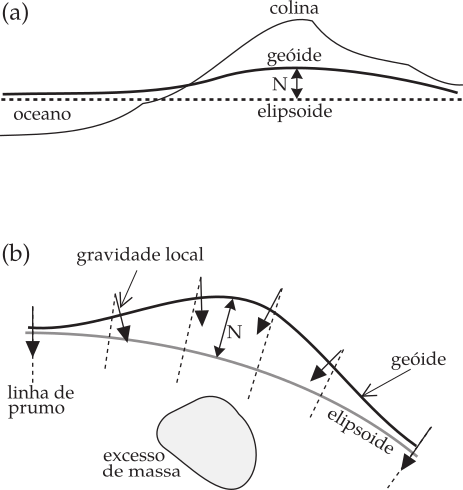
\includegraphics[width=0.4\linewidth]{fig/Fig_02.25} 

}

\caption{(a) Uma massa fora do elipsoide ou (b) um excesso de massa abaixo do elipsoide eleva o geoide acima do elipsoide. N é a ondulação do geoide. }\label{fig:massa}
\end{figure}

\hypertarget{ondulacoes-do-geoide}{%
\subsubsection{Ondulações do geoide}\label{ondulacoes-do-geoide}}

Ao computar a figura teórica da Terra, a distribuição de massa abaixo do elipsoide é assumido como homogêneo. Um excesso local de massa sob o elipsoide irá desviar e fortalecer a gravidade localmente. O potencial do elipsoide é alcançado mais longe do centro da Terra. A superfície equipotencial é forçada a se inclinar para cima enquanto permanece normal à gravidade. Isto dá uma ondulação geoide positiva sobre um excesso de massa sob o elipsoide (Figura \ref{fig:massa}b). Por outro lado, um déficit de massa abaixo do elipsoide irá desviar o geoide abaixo do elipsoide, causando uma ondulação geoidal negativa. Como resultado da topografia irregular e da distribuição de massa interna heterogênea da Terra, o geoide é uma superfície equipotencial acidentada.

O potencial do geoide é representado matematicamente por \textbf{funções harmônicas esféricas} que envolvem os \textbf{polinômios associados de Legendre}. Estes são mais complicados que os polinômios comuns de Legendre usados para descrever o potencial gravitacional do elipsoide (Equações. \eqref{eq:0223} - \eqref{eq:0225}). Até agora só consideramos variação do potencial com distância \(r\) e com o ângulo de colatitude \(\theta\). Isso é uma simplificação excessiva, porque as variações de densidade dentro da Terra não são simétricas em relação ao eixo de rotação. O geoide é uma superfície equipotencial para a distribuição da densidade real na Terra, e assim o potencial do geoide varia com a longitude e com a co-latitude. Essas variações são consideradas expressando o potencial como soma das funções harmônicas esféricas, conforme descrito. Esta representação do geopotencial é análoga à expressão mais simples do potencial gravitacional da Terra rotacionalmente simétrica usando uma série de polinômios de Legendre (Equação \eqref{eq:0225}).

Em análises modernas, o coeficiente de cada termo no geopotencial - semelhante aos coeficientes \(J_n\) na Equação \eqref{eq:0225} - pode ser calculado até um alto grau harmônico. Os termos até um grau selecionado são então usados para calcular um modelo do geoide e do campo de gravidade da Terra. Uma combinação de dados de satélite e medidas de gravidade da superfície foi usada para construir o Modelo da Terra Goddard - Goddard Earth Model (GEM)10. Uma comparação global entre um elipsoide de referência com o aplanamento \(1/298.257\) e a superfície geoide calculada a partir do modelo GEM 10 mostra ondulações geoidais de longo comprimento de onda (Figura \ref{fig:ondulacao}). A maior ondulação negativa (\(-105\) m) está no Oceano Índico, ao sul da Índia, e a maior ondulação positiva (\(+73\) m) está no Oceano Pacífico equatorial, ao norte da Austrália. Essas características de grande escala são muito amplas para serem atribuídas a anomalias de massa crostais ou litosféricas. Eles são pensados serem devido a heterogeneidades que se estendem profundamente no manto inferior, mas sua origem ainda não é compreendida.

\begin{figure}

{\centering 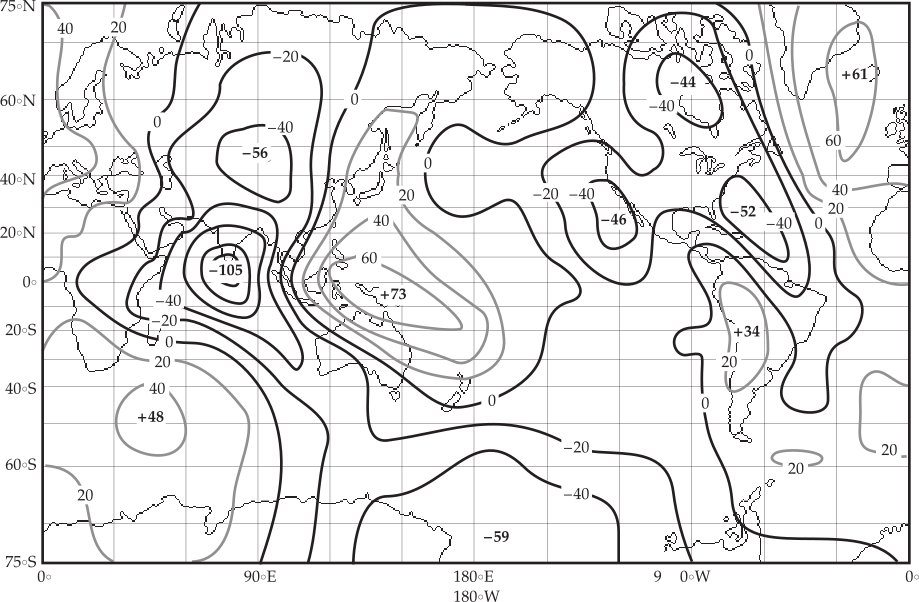
\includegraphics[width=0.8\linewidth]{fig/Fig_02.26} 

}

\caption{Mapa mundi das ondulações geoidais relativas a um elipsoide de referência de aplanamento $f= 1/298.257$. }\label{fig:ondulacao}
\end{figure}

\hypertarget{anomalias-gravitacionais}{%
\section{Anomalias gravitacionais}\label{anomalias-gravitacionais}}

\hypertarget{introducao}{%
\subsection{introdução}\label{introducao}}

O valor médio da gravidade na superfície da Terra é de aproximadamente \(9.80\,\mathrm{m}\mathrm{s}^{-2}\) ou \(980000\,\mathrm{mgal}\). A rotação e o achatamento da Terra fazem com que a gravidade aumente em aproximadamente \(5300\,\mathrm{mgal}\), do equador ao polo, o que é uma variação de apenas cerca de \(0.5\%\). Assim, as medidas de gravidade são de dois tipos. A primeira corresponde à determinação da magnitude absoluta da gravidade em qualquer lugar; e a segunda consiste em medir a mudança na gravidade de um lugar para outro. Em estudos geofísicos, especialmente na prospecção por gravidade, é necessário medir com precisão as variações na gravidade causadas por estruturas subterrâneas. Estes requerem uma sensibilidade instrumental da ordem de \(0.01\,\mathrm{mgal}\). É muito difícil projetar um instrumento para medir o valor absoluto da gravidade que tem essa alta precisão e que também é portátil o suficiente para ser usado facilmente em diferentes lugares. O levantamento de gravidade é geralmente realizado com um instrumento portátil chamado gravímetro, que determina a variação da gravidade em relação a um ou mais locais de referência. Em levantamentos de gravidade, as variações relativas determinadas com um gravímetro podem ser convertidas em valores absolutos por calibração com medições absolutas feitas em estações selecionadas.

\hypertarget{medida-absoluta-da-gravidade}{%
\subsection{Medida absoluta da gravidade}\label{medida-absoluta-da-gravidade}}

O método clássico de medir a gravidade é com um pêndulo. Um pêndulo simples consiste em um peso suspenso no fim de uma fina fibra. O pêndulo composto (ou reversível), descrito pela primeira vez por Henry Kater em 1818, permite medições mais exatas. Consiste numa haste de metal duro ou de quartzo, com cerca de \(50\,\mathrm{cm}\) de comprimento, à qual está ligada uma massa móvel. Perto de cada extremidade da haste é fixado um pivô, que consiste em uma ponta de faca de quartzo apoiada em um plano de quartzo plano. O período do pêndulo é medido por oscilações sobre um dos pivôs. O pêndulo é então invertido e seu período em torno do outro pivô é determinado. A posição da massa móvel é ajustada até os períodos próximos dos dois pivôs serem iguais. A distância \(L\) entre os pivôs é então medida com precisão. O período do instrumento é dado por

\begin{equation}
T=2 \pi \sqrt{\frac{I}{m g h}}=2 \pi \sqrt{\frac{L}{g}}  \label{eq:0234}
\end{equation}

onde \(I\) é o momento de inércia do pêndulo em torno de um pivô, \(h\) é a distância do centro de massa do pivô, e \(m\) é a massa do pêndulo. Conhecer o comprimento \(L\) do método de Kater evita o conhecimento de \(I\), \(m\) e \(h\).

A sensibilidade do pêndulo composto é encontrada diferenciando a (Equação \eqref{eq:0234}). Isto dá

\begin{equation}
\frac{\Delta g}{g}=-2 \frac{\Delta T}{T} \label{eq:0235}
\end{equation}

Para obter uma sensibilidade de cerca de \(1\,\mathrm{mgal}\) é necessário determinar o período com uma precisão de cerca de \(0.5 \,\mathrm{s}\). Isto pode ser conseguido facilmente hoje com relógios atômicos precisos. O pêndulo composto foi o principal instrumento para a prospecção da gravidade nos anos de 1930, quando o tempo das oscilações era precisamente mais difícil. Era necessário marcar com a maior precisão possível um número muito grande de oscilações. Como resultado, uma única medição de gravidade demorava cerca de meia hora.

O desempenho do instrumento foi prejudicado por vários fatores. A reação inercial do invólucro à massa oscilante do pêndulo foi compensada pela montagem de dois pêndulos no mesmo chassi e balançando-os em fase oposta. A resistência do ar foi reduzida

alojando a montagem do pêndulo em uma câmara a vácuo controlada termostaticamente. A fricção no pivô era minimizado pelo fio de faca de quartzo e plano, mas devido ao desnível menor, a borda de contato não foi exatamente repetida se o conjunto foi montado em um local diferente, que afetou a confiabilidade das medições. o aparelho era volumoso, mas foi usado até a década de 1950 como o método principal de fazer medições de gravidade absoluta.

\hypertarget{medidas-relativas-da-gravidade-o-gravimetro}{%
\subsection{Medidas relativas da gravidade: o gravímetro}\label{medidas-relativas-da-gravidade-o-gravimetro}}

Em princípio, um medidor de gravidade ou gravímetro é um balança de equilíbrio muito sensível. Os primeiros gravímetros foram baseados na aplicação direta da lei de Hooke. Uma massa \(m\) suspendida por uma mola de comprimento \(s_0\) faz com que ela se estique até um novo comprimento \(s\). A extensão, ou mudança de comprimento, da mola é proporcional à força restauradora da mola e, portanto, ao valor da gravidade, de acordo com:

\begin{align}
F=m g=-k\left(s-s_{0}\right). \label{eq:0236}
\end{align}

onde \(k\) é a constante elástica da mola. O gravímetro é calibrado em um local conhecido. Se a gravidade é diferente em outro local, a extensão das molas variam e a partir disso, a mudança na gravidade pode ser calculada.

Este tipo de gravímetro, baseado diretamente na lei de Hooke, é chamado de tipo estável. Ele foi substituído por do tipos instáveis ou astatizados, que são construídos de maneira que uma força adicional atua na mesma direção que a gravidade e se opõe à força restauradora da mola. o instrumento está então em um estado de equilíbrio instável. este condição é realizada através do projeto da mola. E se o comprimento natural \(s_0\) pode ser tão menor quanto possível, idealmente zero, Equação \eqref{eq:0236} mostra que a força restauradora é então proporcional ao comprimento físico da mola em vez de sua extensão. A \emph{mola de comprimento zero}, primeiro introduzida no gravímetro LaCoste-Romberg, é agora um elemento comum em gravímetros modernos. A mola é geralmente do tipo helicoidal. Quando uma mola helicoidal é esticada, a fibra da mola é torcida; a torção total ao longo do comprimento da fibra é igual à extensão do mola como um todo. Durante a fabricação de uma mola helicoidal de comprimento zero é dado uma torção extra, de modo que a sua a tendência é desenrolar. Um aumento na gravidade estica o mola contra sua força restauradora, e a extensão é aumentada pela pré-tensão interna.

\begin{figure}

{\centering 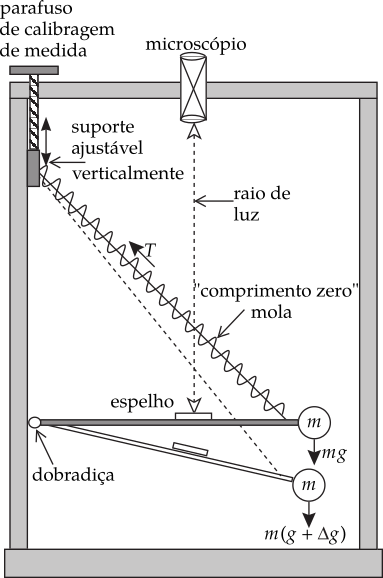
\includegraphics[width=0.4\linewidth]{fig/Fig_02.27} 

}

\caption{Princípio de operação de um gravímetro do tipo instavel (astatizado)}\label{fig:gravimetro}
\end{figure}

A operação de um gravímetro é ilustrada na Figura \ref{fig:gravimetro}. Uma massa é suportada por uma barra horizontal na qual um espelho é anexado. A posição da haste é observada com um feixe de luz refletido em um microscópio. Se a gravidade mudar, a mola de comprimento zero é prolongada ou encurtada e a posição da haste é alterada, o que desvia o raio de luz. O princípio de deflexão nula é utilizado. Um parafuso de ajuste altera a posição da fixação superior da mola, o que altera sua tensão e restaura a haste para sua posição horizontal original, conforme detectado pelo raio de luz e pelo microscópio. As voltas do parafuso de ajuste são calibradas em unidades da mudança de gravidade, geralmente em \(\mathrm{mgal}\).

O gravímetro é leve, robusto e portátil. Após o nivelamento inicial do instrumento, uma medição precisa de uma diferença de gravidade pode ser feita em poucos minutos. o o gravímetro tem uma sensibilidade de cerca de \(0.01\, \mathrm{mgal}\) \((10\,\mu\mathrm{gal})\). Essa alta sensibilidade faz com que seja suscetível a pequenas alterações em suas próprias propriedades.

\hypertarget{levantamentos-gravimetricos}{%
\subsection{Levantamentos gravimétricos}\label{levantamentos-gravimetricos}}

Se um gravímetro for montado em um determinado local e monitorado por cerca de uma hora, as leituras repetidas variam suavemente com o tempo. As alterações somam vários centésimos de mgal. O \emph{desvio instrumental} é parcialmente devida a mudanças induzidas termicamente nas propriedades elásticas da mola gravimétrica, que são minimizadas ao alojar os elementos críticos em uma câmara evacuada. Além disso, as propriedades elásticas da mola não são perfeitas, mas fluem lentamente com o tempo. O efeito é pequeno nos gravímetros modernos e pode ser compensado fazendo uma \emph{correção de desvio (drift correction)}. Isto é obtido pela ocupação repetida de algumas estações de medição em intervalos durante o dia Figura \ref{fig:drift}

\begin{figure}

{\centering 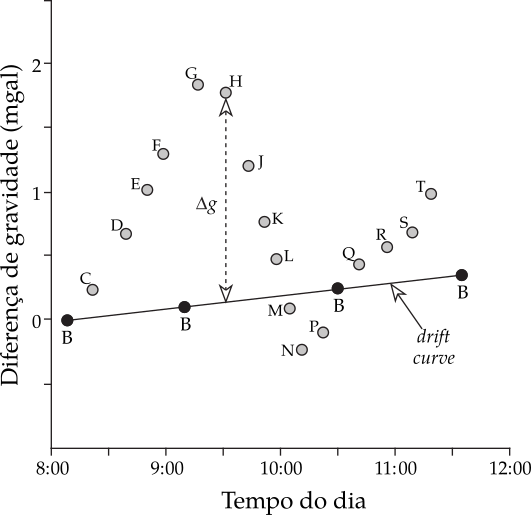
\includegraphics[width=0.4\linewidth]{fig/Fig_02.28} 

}

\caption{Compensação de leituras de gravidade para desvio instrumental. As estações de gravidade B – T são ocupadas em sequência em tempos conhecidos. As medições repetidas na estação base B permitem que uma correção de desvio seja feita nas leituras de gravidade nas outras estações.}\label{fig:drift}
\end{figure}

Leituras de gravidade em outras estações são ajustadas por comparação com a curva de desvio. Para fazer esta correção, o tempo de cada medição deve ser anotado.

Durante o dia, enquanto as medições estão sendo feitas, o gravímetro está sujeito à atração de maré, incluindo o deslocamento vertical devido às marés orgânicas da Terra. A teoria das marés é bem conhecida e seu efeito dependente do tempo na gravidade pode ser calculado precisamente para qualquer lugar na Terra a qualquer momento. Novamente, a \emph{correção das marés} requer que o tempo de cada medição seja conhecido.

O objetivo do levantamento por gravidade é localizar e descrever estruturas subsuperficiais a partir dos efeitos de gravidade causados por suas densidades anômalas. Mais comumente, as medições gravimétricas são feitas em uma rede de estações, espaçadas de acordo com a finalidade da pesquisa. Em estudos ambientais, uma investigação detalhada de alta resolução da expressão gravitacional de uma pequena área requer pequenas distâncias de alguns metros entre as estações de medição. Em levantamentos de gravidade regional, usados para a definição de estruturas ocultas de interesse comercial prospectivo, a distância entre as estações pode ser de vários quilômetros. Se a área pesquisada não for muito grande, um local adequado é selecionado como estação base (ou local de referência), e as diferenças de gravidade entre os locais pesquisados e este site são medidas. Em um levantamento de gravidade em escala nacional, as diferenças de gravidade podem ser determinadas em relação a um local onde o valor absoluto da gravidade é conhecido.

\hypertarget{correcoes-de-medidas-gravimetricas}{%
\subsection{Correções de medidas gravimétricas}\label{correcoes-de-medidas-gravimetricas}}

Se o interior da Terra fosse uniforme, o valor da gravidade no elipsoide de referência internacional variaria com a latitude de acordo com a fórmula da gravidade normal (Equação \eqref{eq:0230}). Isso nos fornece um valor de referência para medições de gravidade. Na prática, não é possível medir a gravidade no elipsoide no local onde o valor de referência é conhecido. A elevação de uma estação de medição pode estar a centenas de metros acima ou abaixo do elipsoide. Além disso, a estação de gravidade pode ser cercada por montanhas e vales que perturbam a medição. Por exemplo, se P e Q representam estações de gravidade em diferentes altitudes em terrenos acidentados (Figura \ref{fig:correcao}a). O valor teórico da gravidade é calculado nos pontos R no elipsoide de referência abaixo de P e Q. Assim, devemos corrigir a gravidade medida antes que ela possa ser comparada com o valor de referência.

O topo do morro adjacente às estações P e Q tem um centro de massa que fica mais alto do que a elevação da medição (Figura \ref{fig:correcao}a). O gravímetro mede a gravidade na direção vertical, ao longo da linha de prumo local. A massa do topo da colina acima de P atrai o gravímetro e causa uma aceleração com um componente vertical para cima em P. A gravidade medida é reduzida pela presença do topo da colina; Para compensar isso, uma correção de terreno (ou topográfica) é calculada e adicionada à gravidade medida. Um efeito semelhante é observado em Q, mas o topo da colina acima de Q é menor e a correção de terreno correspondente é menor. Essas correções efetivamente nivelam a topografia para a mesma elevação da estação gravimétrica. A presença de um vale ao lado de cada estação de medição também requer uma correção do terreno. Neste caso, imaginemos que poderíamos encher o vale até o nível de cada estação com rochas da mesma densidade que está abaixo de P e Q. A atração para baixo no gravímetro seria aumentada, então a correção do terreno para um vale também deve ser adicionado à gravidade medida, tal como para uma colina. Remover os efeitos da topografia em torno de uma estação de gravidade requer a realização de correções de terreno positivas \(\left(\Delta g_{\mathrm{T}}\right)\) para as colinas e vales.

Depois de nivelar a topografia, há agora uma camada fictícia uniforme de rocha com densidade \(\rho\) entre a estação de gravidade e o elipsoide de referência (Figura \ref{fig:correcao}b). A aceleração gravitacional dessa massa rochosa está incluída na medida da gravidade e deve ser removido antes que possamos comparar com a gravidade teórica. A camada é considerada como sendo um disco plano ou placa de espessura \(h_{\mathrm{P}}\) ou \(h_{\mathrm{Q}}\) em cada estação; é chamado o \emph{placa Bouguer}. Sua aceleração gravitacional pode ser calculada para espessura e densidade conhecidas \(\rho\), e fornece uma \emph{correção de placa Bouguer} \(\left(\Delta g_{\mathrm{BP}}\right)\) que deve ser subtraída da gravidade medida, se a estação de gravidade estiver acima do nível do mar. Note que, se a estação de gravidade estiver abaixo do nível do mar, nós temos que preencher o espaço acima dela até o nível do mar com a rocha de densidade \(\rho\); isso requer aumentar a gravidade medida correspondentemente. A correção da placa de Bouguer \(\left(\Delta g_{\mathrm{BP}}\right)\) é negativa se a estação estiver acima do nível do mar, mas positiva se estiver abaixo do nível do mar. Seu tamanho depende da densidade das rochas locais, mas normalmente equivale a cerca de \(0.1\,\mathrm{mgal}\, \mathrm{m}^{-1}\).

\begin{figure}

{\centering 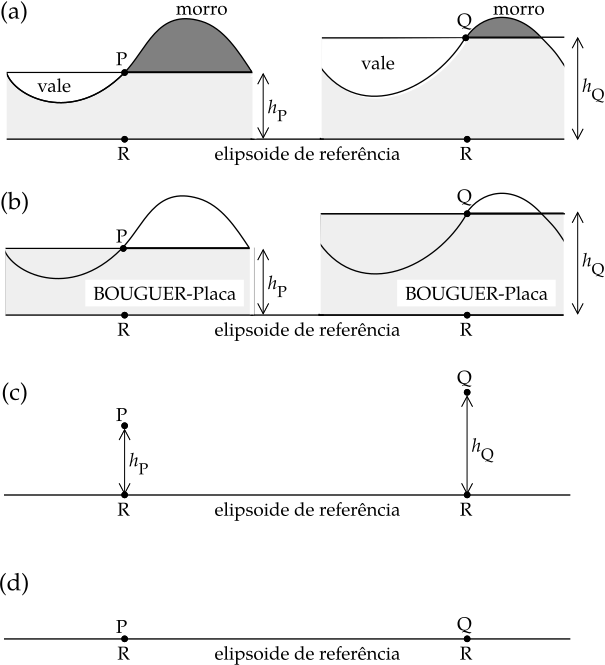
\includegraphics[width=0.6\linewidth]{fig/Fig_02.29} 

}

\caption{Após (a) correções do terreno, (b) correção da placa Bouguer, e (c) correção do ar livre, as medidas de gravidade nas estações P e Q podem ser comparadas com (d) a gravidade teórica em R no elipsoide de referência.}\label{fig:correcao}
\end{figure}

Finalmente, devemos compensar a gravidade medida para a elevação \(h_{\mathrm{P}}\) ou \(h_{\mathrm{Q}}\) da estação de gravidade acima do elipsoide (Figura \ref{fig:correcao}c). A parte principal da gravidade é devida à atração gravitacional, que diminui proporcionalmente ao quadrado inverso da distância do centro da Terra. A gravidade medida em \(P\) ou \(Q\) é menor do que seria se medida no elipsoide em \(R\). Uma \emph{correção de ar livre (free-air)} \(\left(\Delta g_{\mathrm{FA}}\right)\) para a elevação da estação deve ser adicionada à gravidade medida. Esta correção ignora os efeitos do material entre os níveis de medição e referência, pois isso é considerado em \(\Delta g_{\mathrm{BP}}\). Observe que, se a estação de gravidade estivesse abaixo do nível do mar, a parte gravitacional da gravidade medida seria muito grande em comparação com o elipsoide de referência; precisaríamos subtrair \(\left(\Delta g_{\mathrm{FA}}\right)\) neste caso. A correção de ar livre é positiva se a estação estiver acima do nível do mar, mas negativa se estiver abaixo do nível do mar (como pode ser o caso no Vale da Morte ou ao lado do Mar Morto). Isso equivale a cerca de 0.3 \(\mathrm{mgal}\, \mathrm{m}^{-1}\).

A correção de ar livre é sempre de sentido oposto à correção da placa de Bouguer. Por conveniência, os dois são frequentemente combinados em uma única correção de elevação, que equivale a cerca de 0.2 \(\mathrm{mgal}\, \mathrm{m}^{-1}\). Isto deve ser adicionado para as estações de gravidade acima do nível do mar e subtraído se a gravidade for medida abaixo do nível do mar. Além disso, uma correção de maré \(\left(\Delta g_{\text { tile }}\right)\) deve ser feita e, se a gravidade for medida em um veículo em movimento, a correção de Eötvõs também é necessária.

Após a correção, a gravidade medida pode ser comparada com a gravidade teórica no elipsoide (Figura \ref{fig:correcao}b). Note que o procedimento acima reduz a gravidade medida para a superfície do elipsoide. Em princípio, é igualmente válido corrigir a gravidade teórica do elipsoide para cima até o nível em que a medição foi feita. Este método é preferido em tipos mais avançados de análise de anomalias de gravidade, onde a possibilidade de uma massa anômala entre o elipsoide e a superfície do solo deve ser levada em conta.

\hypertarget{correcoes-de-latitude}{%
\subsubsection{Correções de latitude}\label{correcoes-de-latitude}}

A gravidade teórica a uma determinada latitude é dada pela fórmula de gravidade normal (Equação \eqref{eq:0230}). Se a gravidade medida for um valor absoluto, a correção da latitude é feita subtraindo o valor previsto por esta fórmula. Muitas vezes, no entanto, o levantamento da gravidade é feito com um gravímetro, e a quantidade medida, \(g_m\), é a diferença de gravidade relativa a uma estação base. A gravidade de referência normal \(g_n\) pode então ser substituída por uma correção de latitude, obtida pela diferenciação da Equação \eqref{eq:0230}:

\begin{align}
\frac{\partial g_{n}}{\partial \lambda}=g_{e}\left(\beta_{1} \sin 2 \lambda+\beta_{2} \sin 4 \lambda\right)
\label{eq:0237}
\end{align}

Depois de converter \(\partial \lambda\) de radianos em quilômetros e desprezar o termo \(\beta_2\), a correção de latitude \(\left(\Delta g_{\mathrm{lat}}\right)\) é 0.8140 \(\sin 2 \lambda\, \mathrm{mgal}\) por quilômetro de deslocamento norte-sul. Como a gravidade diminui em direção aos pólos, a correção para estações mais próximas do polo do que a estação base deve ser adicionada à gravidade medida.

\hypertarget{correcao-do-terreno}{%
\subsubsection{Correção do terreno}\label{correcao-do-terreno}}

A correção do terreno \(\left(\Delta g_{\mathrm{T}}\right)\) para uma colina adjacente a uma estação de gravidade é calculada dividindo a colina em vários prismas verticais (Figura \ref{fig:terreno}a). A contribuição de cada elemento vertical para a aceleração vertical no ponto de observação \(P\) é calculada assumindo simetria cilíndrica sobre \(P\). A altura do prisma é \(h\), seus raios interno e externo são \(r_1\) e \(r_2\), respectivamente, o ângulo subentendido em \(P\) é \(\phi_0\), e a densidade da colina é \(\rho\) (Figura \ref{fig:terreno}b). Deixe os lados de um pequeno elemento cilíndrico serem \(dr\), \(dz\) e \(r d\phi\); sua massa é \(dm= \rho r d\phi dr dz\) e sua contribuição para a aceleração ascendente causada pelo prisma em P é

\begin{align}
\Delta g=G \frac{\mathrm{d} m}{\left(r^{2}+z^{2}\right)} \cos \theta=G \frac{\rho r \mathrm{d} r \mathrm{d} z \mathrm{d} \phi}{\left(r^{2}+z^{2}\right)} \frac{z}{\sqrt{\left(r^{2}+z^{2}\right)}} \label{eq:0238}
\end{align}

Combinando e rearranjando termos e a ordem de integração, obtém-se a aceleração ascendente em \(P\) devido ao prisma cilíndrico:

\begin{align}
\Delta g_{\mathrm{T}}=G \rho \int_{\phi=0}^{\phi_{0}} \mathrm{d} \phi \int_{r=r_{1}}^{r_{2}}\left(\int_{z=0}^{h} \frac{z \mathrm{d} z}{\left(r^{2}+z^{2}\right)^{3 / 2}}\right) r \mathrm{d} r \label{eq:0239}
\end{align}

A integração sobre \(\phi\) dá \(\phi_0\); após integração adicional sobre \(z\) conseguimos:

\begin{align}
\Delta g_{T}=G \rho \phi_{0} \int_{r=r_{1}}^{r_{2}}\left(\frac{r}{\sqrt{\left(r^{2}+h^{2}\right)}}-1\right) \mathrm{d} r \label{eq:0240}
\end{align}

A integração sobre \(r\) fornece a aceleração ascendente produzida em \(P\) pelo cilindro:

\begin{align}
\Delta g_{T}=G \rho \phi_{0}\left(\left(\sqrt{r^{2}+h^{2}}-r_{1}\right)-\left(\sqrt{r^{2}+h^{2}}-r_{2}\right)\right) \label{eq:0241}
\end{align}

A direção de \(\Delta g_{\mathrm{T}}\) na (Figura \ref{fig:terreno}b) é para cima, oposta à gravidade; a correção do terreno correspondente deve ser adicionada à gravidade medida.

Na prática, as correções de terreno podem ser feitas usando um gráfico de terreno (Figura \ref{fig:terreno}c) no qual círculos concêntricos e linhas radiais dividem a área ao redor da estação de gravidade em setores que possuem simetria radial como a seção transversal do elemento de um cilindro vertical. Na Figura \ref{fig:terreno}b. Os raios interno e externo de cada setor correspondem a \(r_1\) e \(r_2\) e o ângulo subtendido pelo setor é \(\phi\). A correção do terreno para cada setor dentro de cada zona é pré-calculada usando a Equação \eqref{eq:0241} e tabulado. O gráfico é desenhado em uma folha transparente que é sobreposta em um mapa topográfico na mesma escala e centrada na estação de gravidade. A elevação média dentro de cada setor é estimada com a maior precisão possível, e a diferença de elevação (ou seja, \(h\) na Equação \eqref{eq:0241}) do setor em relação à estação é calculada. Isso é multiplicado pelo fator de correção do setor para dar sua contribuição para a correção do terreno. Finalmente, a correção do terreno na estação gravitacional é obtida pela soma das contribuições de todos os setores. O procedimento deve ser repetido para cada estação de gravidade.

Quando o gráfico de terreno está centrado numa nova estação, o relevo topográfico médio dentro de cada setor muda e deve ser calculado de novo. Como resultado, as correções do terreno são demoradas e tediosas. Os efeitos mais importantes vêm da topografia mais próxima da estação. No entanto, as correções do terreno são geralmente necessárias se uma diferença topográfica dentro de um setor estiver a mais de 5\% de sua distância da estação.

\begin{figure}

{\centering 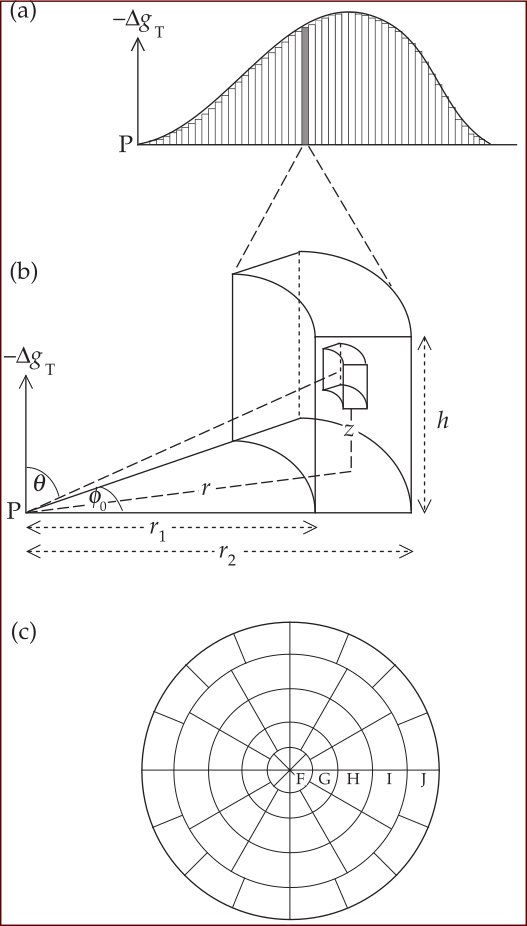
\includegraphics[width=0.6\linewidth]{fig/Fig_02.30} 

}

\caption{As correções de terreno $\Delta g_\mathrm{T}$ são feitas (a) dividindo a topografia em elementos verticais, (b) computando a correção para cada elemento cilíndrico de acordo com sua altura acima ou abaixo da estação de medição e (c) somando as contribuições para todos os elementos ao redor a estação com o auxílio de uma sobreposição transparente em um mapa topográfico.}\label{fig:terreno}
\end{figure}

\hypertarget{correcao-bouger-placa-bouger}{%
\subsubsection{Correção Bouger (placa Bouger)}\label{correcao-bouger-placa-bouger}}

A correção da placa Bouguer \(\left(\Delta g_{\mathrm{BP}}\right)\) compensa o efeito de uma camada de rocha cuja espessura corresponde à diferença de elevação entre os níveis de medição e referência. Isto é modelado por um disco sólido de densidade \(\rho\) e raio infinito centrado na estação gravitacional \(P\). A correção é computada por extensão do cálculo para a correção do terreno. Um prisma cilíndrico elementar é definido como na Figura \ref{fig:terreno}b. Seja o ângulo \(\phi\) subtendido pelo prisma aumentar para \(2\pi\) e o raio interno diminuir para zero; o primeiro termo entre parênteses na Equação \eqref{eq:0241}) reduz para \(h\). A aceleração gravitacional no centro de um disco sólido de raio r é então

\begin{align}
\Delta g_{\mathrm{T}}=2 \pi G \rho\left(h-\left(\sqrt{r^{2}+h^{2}}-r\right)\right) \label{eq:0242}
\end{align}

Agora seja o raio \(r\) do disco aumentar. O valor de \(h\) torna-se gradualmente insignificante comparado a \(r\); no limite, quando \(r\) é infinito, o segundo termo na Equação \eqref{eq:0242}) tende a zero. Assim, a correção da placa de Bouguer \(\left(\Delta g_{\mathrm{BP}}\right)\) é dada por

\begin{align}
\Delta g_{\mathrm{BP}}=2 \pi G \rho h \label{eq:0243}
\end{align}

Inseririndo valores numéricos dá \(0.0419\times 10^{-3}\,\rho\, \mathrm{mgal} \,\mathrm{m}^{-1}\) para \(\left(\Delta g_{\mathrm{BP}}\right)\), onde a densidade \(\rho\) está em \(\mathrm{kg}\mathrm{m}^{-3}\). A escolha correta da densidade é muito importante no cálculo de \(\left(\Delta g_{\mathrm{BP}}\right)\) e \(\left(\Delta g_{\mathrm{T}}\right)\). Alguns métodos para determinar a melhor escolha são descritos em detalhes abaixo.

Uma consideração adicional é necessária em pesquisas de gravidade marinha. \(\left(\Delta g_{\mathrm{BP}}\right)\) requer densidade uniforme abaixo da superfície do elipsoide de referência. Para calcular a \(\left(\Delta g_{\mathrm{BP}}\right)\) sobre uma região oceânica, devemos, com efeito, substituir a água do mar pela rocha de densidade \(\rho\). No entanto, a gravidade medida contém um componente devido à atração da água do mar (densidade 1030 \(\mathrm{kg}\,\mathrm{m}^{-3}\)) na bacia oceânica. A correção da placa Bouguer em levantamentos de gravidade marinha é feita substituindo a densidade \(\rho\) na Equação \eqref{eq:0243}) por \((\rho - 1030)\;\mathrm{kg}\,\mathrm{m}^{-3}\). Quando um levantamento por gravidade a bordo é feito sobre um lago grande e profundo, uma tolerância similar deve ser feita para a profundidade da água no lago usando uma densidade presumida de \((\rho - 1000)\;\mathrm{kg}\,\mathrm{m}^{-3}\).

\hypertarget{correcao-ar-livre-free-air}{%
\subsubsection{Correção ar livre (free-air)}\label{correcao-ar-livre-free-air}}

A correção de ar livre \(\left(\Delta g_{\mathrm{FA}}\right)\) tem um título bastante colorido, mas um pouco enganador, dando a impressão de que a estação de medição está flutuando no ar acima do elipsoide. A densidade do ar à temperatura e pressão padrão é de cerca de 1.3 \(\mathrm{kg}\,\mathrm{m}^{-3}\) e uma massa de ar entre os níveis de observação e referência causaria um efeito de gravidade detetável de cerca de \(50\,\mu\mathrm{gal}\) a uma elevação de \(1000\,\mathrm{m}\). De fato, a correção de ar livre não presta atenção à densidade do material entre a elevação da medição e o elipsoide. É uma correção direta para a diminuição da aceleração gravitacional com a distância do centro da Terra:

\begin{align}
\frac{\partial g}{\partial r}=\frac{\partial}{\partial r}\left(-G \frac{E}{r^{2}}\right)=+2 G \frac{E}{r^{3}}=-\frac{2}{r} g \label{eq:0244}
\end{align}

Ao substituir o raio da Terra (6371 km) por \(r\) e o valor médio da gravidade \((981,000\, \mathrm{mgal})\) por \(g\), o valor de \(\Delta g_{\mathrm{FA}}\) é encontrado ser de \(0.3086\,\mathrm{mgal}\,\mathrm{m}^{-1}\).

\hypertarget{correcao-de-elevacao-combinada}{%
\subsubsection{Correção de elevação combinada}\label{correcao-de-elevacao-combinada}}

As correções da placa de ar livre e Bouguer são frequentemente combinadas em uma única correção de elevação, que é \((0.3086 - (0.0419\rho\times 10^{-3}))\) \(\mathrm{mgal}\,\mathrm{m}^{-1}\). A substituição de uma densidade típica por rochas crustais, geralmente considerada como sendo 2670 \(\mathrm{kg}\,\mathrm{m}^{-3}\), fornece uma correção de elevação combinada de \(0.197\;\mathrm{mgal}\,\mathrm{m}^{-1}\). Isto deve ser adicionado à gravidade medida se a estação está acima do elipsoide e é subtraída se estiver abaixo.

A alta sensibilidade dos gravímetros modernos permite uma precisão alcançável de \(0.01 - 0.02\;\mathrm{mgal}\) nos levantamentos de gravidade modernos. Para alcançar essa precisão, as correções das variações de gravidade com latitude e elevação devem ser feitas com exatidão. Isso requer que as coordenadas precisas de uma estação de gravidade sejam determinadas por levantamentos geodésicos precisos. A precisão necessária do posicionamento horizontal é indicada pela correção de latitude. Este é o máximo a \(45^\circ\) latitudes, onde, para atingir uma precisão de pesquisa de \(\pm 0.01\; \mathrm{mgal}\), as posições norte-sul das estações de gravidade devem ser conhecidas por cerca de \(\pm 10\,\mathrm{m}\). A precisão necessária no posicionamento vertical é indicada pela correção de elevação combinada de \(0.2\,\mathrm{mgal}\,\mathrm{m}^{-1}\). Para alcançar uma precisão em um levantamento de \(\pm 0.01\; \mathrm{mgal}\), a elevação do gravímetro acima do elipsoide de referência deve ser conhecida a cerca de \(\pm 5\, \mathrm{cm}\).

A elevação de um local acima do elipsoide é frequentemente considerada como sendo sua altitude acima do nível médio do mar. No entanto, o nível médio do mar é igualado ao geóide e não ao elipsoide. As ondulações geoidais podem chegar a dezenas de metros. Eles são recursos de longo comprimento de onda. Em um levantamento local, a distância entre o geóide e o elipsoide provavelmente não varia muito, e as diferenças de gravidade da estação base selecionada provavelmente não serão afetadas fortemente. Em uma pesquisa nacional, as discrepâncias devido a ondulações geoidais podem ser mais sérias. No caso de ondulações geoidais serem grandes o suficiente para afetar um levantamento, as altitudes das estações devem ser corrigidas para elevações reais acima do elipsoide.

\hypertarget{densidade-das-rochas}{%
\section{Densidade das rochas}\label{densidade-das-rochas}}

A densidade de rochas na vizinhança de um perfil de gravidade é importante para o cálculo da placa Bouguer e das correções do terreno. Densidade é definida como a massa por unidade de volume de um material. Ela tem diferentes unidades e diferentes valores numéricos no c.g.s. e sistemas SI. Por exemplo, a densidade da água é de \(1\; \mathrm{g} \mathrm{cm}^{-3}\) no sistema c.g.s., mas \(1000\; \mathrm{kgm}^{-3}\) no sistema SI. Na prospecção por gravidade unidades como c.g.s. ainda estão em uso comum, mas estão sendo lentamente substituídas por unidades do SI. As fórmulas dadas para \(\Delta g_{\mathrm{T}}\) e \(\Delta g_{\mathrm{BP}}\) nas Equações \eqref{eq:0241} e \eqref{eq:0243}, respectivamente, exigem que a densidade seja dada em \(\mathrm{kg}\, \mathrm{m}^{-3}\).

Uma maneira simples de determinar a densidade apropriada para usar em um estudo de gravidade é fazer uma coleção representativa de amostras de rochas com o auxílio de um mapa geológico. A gravidade específica de uma amostra pode ser encontrada diretamente pesando-a primeiro no ar e depois na água, e aplicando o princípio de Arquimedes. Isto dá sua densidade \(\rho_\mathrm{r}\) em relação à da água:

\begin{align}
\rho_{\mathrm{r}}=\frac{W_{\mathrm{a}}}{W_{\mathrm{a}}-W_{\mathrm{w}}} \label{eq:0245}
\end{align}

Tipicamente, as densidades encontradas para diferentes tipos de rochas por este método mostram uma grande quantidade de dispersão sobre suas médias, e as faixas de valores para diferentes tipos de rochas se sobrepõem (Figura \ref{fig:densidade}). As densidades das rochas ígneas e metamórficas são geralmente mais altas que as das rochas sedimentares. Este método é adequado para o reconhecimento de uma área. Infelizmente, muitas vezes é difícil garantir que a coleção superficial de rochas seja representativa dos tipos de rochas em estruturas subsuperficiais, de modo que métodos alternativos de determinação da densidade apropriada são geralmente empregados. A densidade pode ser medida em furos verticais, perfurados para explorar a natureza de uma estrutura presumida. A densidade determinada no poço é usada para refinar a interpretação da estrutura.

\begin{figure}

{\centering 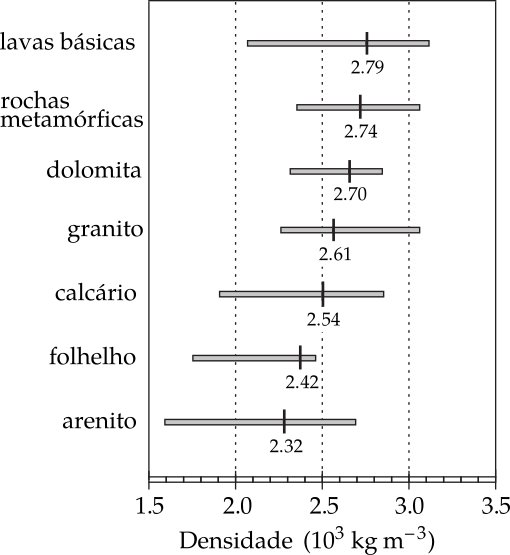
\includegraphics[width=0.6\linewidth]{fig/Fig_02.31} 

}

\caption{Valores médios típicos e intervalos de densidade para alguns tipos de rochas mais comuns.}\label{fig:densidade}
\end{figure}

\hypertarget{densidade-a-partir-de-velocidades-sismicas}{%
\subsection{Densidade a partir de velocidades sísmicas}\label{densidade-a-partir-de-velocidades-sismicas}}

Medições em amostras de sedimentos saturados de água e rochas sedimentares, e em rochas ígneas e metamórficas, mostram que a densidade e as velocidades da ondas sísmicas P e S estão relacionadas. O ajuste ideal para cada conjunto de dados é uma curva suave (Figura \ref{fig:densidadePS}). Cada curva é idealizada, pois os dados reais contêm uma dispersão considerável. Por esta razão, as curvas são mais adequadas para calcular a densidade média de um corpo crustal grande a partir da sua velocidade sísmica média. Devem ser feitos ajustes para as temperaturas e pressões mais altas em profundidade na Terra, que afetam tanto a densidade quanto os parâmetros elásticos das rochas. No entanto, os efeitos de alta pressão e temperatura só podem ser examinados em experimentos de laboratório em amostras pequenas. Não se sabe até que ponto os resultados são representativos da relação velocidade-densidade in situ em grandes blocos crustais.

\begin{figure}

{\centering 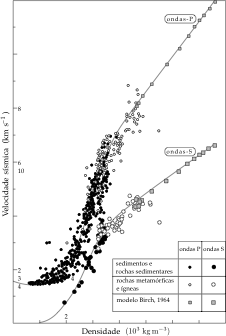
\includegraphics[width=0.6\linewidth]{fig/Fig_02.32} 

}

\caption{relações empíricas entre a densidade e as velocidades das ondas sísmicas P e S em sedimentos saturados de água e rochas sedimentares, rochas ígneas e metamórficas.}\label{fig:densidadePS}
\end{figure}

As curvas velocidade-densidade são relações empíricas que não possuem base teórica. Os dados da onda P são usados mais comumente. Em conjunto com estudos de refração sísmica, eles foram usados para modelar as distribuições de densidade na crosta terrestre e do manto superior responsável por anomalias de gravidade regional em larga escala.

\hypertarget{perfil-de-raio-gama}{%
\subsection{Perfil de raio gama}\label{perfil-de-raio-gama}}

A densidade das formações rochosas adjacentes a um poço pode ser determinada a partir de um instrumento no poço. O princípio faz uso do espalhamento Compton de raios-\(\gamma\) por elétrons fracamente ligados na rocha adjacente a um poço. Um físico americano, Arthur H. Compton, descobriu em 1923 que a radiação espalhada por elétrons frouxamente ligados experimentava um aumento no comprimento de onda. Essa observação simples não pode ser explicada de maneira alguma se a radiação for tratada como uma onda; a radiação espalhada teria o mesmo comprimento de onda que a radiação incidente. O efeito Compton é facilmente explicado considerando a radiação como partículas ou fótons, ou seja, partículas de energia quantificada, em vez de como ondas. A energia de um fóton é inversamente proporcional ao seu comprimento de onda. A colisão de um fóton de raios-\(\gamma\) com um elétron é como uma colisão entre bolas de bilhar; parte da energia do fóton é transferida para o elétron. O fóton espalhado tem menor energia e, portanto, um comprimento de onda maior que o fóton incidente. O efeito Compton foi uma importante verificação da teoria quântica.

O perfilador de densidade, ou perfilador \emph{gamma-gamma} (Figura \ref{fig:gama}), é um dispositivo cilíndrico que contém uma fonte radioativa de raios-\(\gamma\), como \(^{137}\mathrm{Cs}\), que emite radiação através de uma fenda estreita. Os fótons de raios-\(\gamma\) colidem com os elétrons de átomos frouxamente ligados próximos ao buraco e são espalhados. Um contador de cintilação para detectar e medir a intensidade dos raios-\(\gamma\) está localizado na ferramenta a cerca de 45 a 60 cm acima do emissor; a radiação que chega também passa por uma fenda. O emissor e o detector são blindados com chumbo, e a ferramenta é pressionada contra a parede do furo por uma mola forte, de modo que a única radiação registrada é aquela resultante do espalhamento de Compton na formação circundante. A intensidade da radiação detectada é determinada pela densidade dos elétrons e, portanto, pela densidade da rocha próxima à ferramenta de extração. Os raios-\(\gamma\) penetram apenas cerca de 15 cm na rocha.

\begin{figure}

{\centering 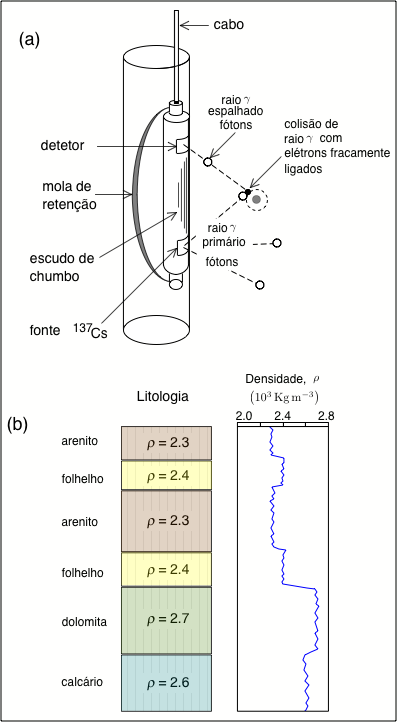
\includegraphics[width=0.6\linewidth]{fig/Fig_02.33} 

}

\caption{(a) O projeto de um dispositivo de um perfil gama-gama para determinar a densidade em um poço e (b) um perfil esquemático gama-gama calibrado em termos da densidade da rocha.}\label{fig:gama}
\end{figure}

Perfis calibrados \emph{gamma-gama} fornecem a densidade aparente da rocha ao redor de um poço. Esta informação é também necessária para calcular a porosidade, que é definida como o volume fracionário da rocha representado por espaços porosos. A maioria das rochas sedimentares é porosa, dependendo a quantidade da quantidade de compactação experimentada. Rochas ígneas e metamórficas geralmente têm baixa porosidade, a menos que tenham sido fraturadas. Normalmente, os poros são preenchidos com ar, gás ou fluido, como água ou óleo. Se as densidades da rocha da matriz e do fluido dos poros são conhecidas, a densidade aparente obtida da extração de \emph{gama-gama} permite que a porosidade da rocha seja determinada.

\hypertarget{gravimetria-de-poco}{%
\subsection{Gravimetria de poço}\label{gravimetria-de-poco}}

A instrumentação moderna permite que a gravidade seja medida com precisão em poços. Um tipo de gravímetro de poço é uma modificação do instrumento LaCoste -- Romberg, adaptado para uso no poço estreito e sob condições de temperatura e pressão elevadas. Instrumentos alternativos foram projetados em diferentes princípios; eles têm uma sensibilidade comparável de cerca de 0.01 mgal. Seu uso para a determinação da densidade do poço é baseado na aplicação das correções de ar livre e da placa Bouguer.

\begin{figure}

{\centering 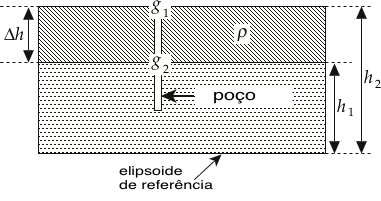
\includegraphics[width=0.6\linewidth]{fig/Fig_02.34} 

}

\caption{Geometria para cálculo da densidade de uma camada rochosa a partir de medições de gravidade feitas em um poço vertical.}\label{fig:camada}
\end{figure}

Sejam \(g_1\) e \(g_2\) os valores de gravidade medidos em um poço vertical nas alturas \(h_1\) e \(h_2\), respectivamente, acima do elipsoide de referência (Figura \ref{fig:camada}). A diferença entre \(g_1\) e \(g_2\) deve-se às diferentes alturas e ao material entre os dois níveis de medição no poó. O valor \(g_2\) será maior que \(g_1\) por dois motivos. Primeiro, porque o nível de medição mais baixo está mais próximo do centro da Terra, \(g_2\) será maior que \(g_1\) pela quantidade da correção de elevação combinada, nominalmente \((0.3086 - (0.0419\rho \times 10^{-3}))\Delta h\) mgal, onde \(\Delta h= h_1-h_2\) Em segundo lugar, no nível inferior \(h_2\), o gravímetro experimenta uma atração Bouguer ascendente devido ao material entre os dois níveis de medição. Isto reduz a gravidade medida em \(h_2\) e requer um aumento de compensação para \(g_2\) de quantidade \((0.0419\rho\times 10^{-3})\Delta h\) mgal. A diferença entre os valores corrigidos de \(g_1\) e \(g_2\) após a redução para o nível \(h_2\) é então

\begin{align}
\begin{aligned} \Delta g &=\left(0.3086-0.0419 \rho \times 10^{-3}\right) \Delta h-0.0419 \rho \times 10^{-3} \Delta h \\ &=\left(0.3086-0.0838 \rho \times 10^{-3}\right) \Delta h \end{aligned}  \label{eq:0246}
\end{align}

O rearranjo desta equação fornece a densidade \(\rho\) do material entre os níveis de medição no poço de sondagem:

\begin{align}
\rho=\left(3.683-11.93 \frac{\Delta g}{\Delta h}\right) \times 10^{3} \mathrm{kg} \mathrm{m}^{-3} \label{eq:0247}
\end{align}

Se as medições da gravidade do poço são feitas com uma precisão de \(\pm 0.01\; \mathrm{mgal}\) a uma separação de cerca de \(10\;\mathrm{m}\), a densidade do material perto do poço pode ser determinada com uma precisão de cerca de \(\pm 10\; \mathrm{kg}\,\mathrm{m}^{-3}\). Mais de \(90 \%\) da variação na gravidade do poço é devido ao material dentro de um raio de cerca de \(5\Delta h\) do poço (cerca de \(50\,\mathrm{m}\) para uma distância \(\Delta h \approx 10\mathrm{m}\) entre os níveis de medição). Isso é muito maior do que a faixa lateral penetrada pelo perfil gama-gama. Como resultado, os efeitos relacionados ao poço em si não são importantes.

\hypertarget{metodo-de-nettleton-para-densidade-proxima-da-superficie}{%
\subsection{Método de Nettleton para densidade próxima da superfície}\label{metodo-de-nettleton-para-densidade-proxima-da-superficie}}

A densidade da superfície próxima do material sob uma colina pode ser determinada por um método criado por L. Nettleton que compara a forma de uma anomalia da gravidade Bouguercom a forma da topografia ao longo de um perfil. O método faz uso da correção de elevação combinada \(\left(\Delta g_{\mathrm{FA}}+\Delta g_{\mathrm{BP}}\right)\) e da correção do terreno \(\left(\Delta g_{\mathrm{T}}\right)\), que são dependentes da densidade. A correção do terreno é menos importante que a correção da placa Bouguer e geralmente pode ser negligenciada.

\begin{figure}

{\centering 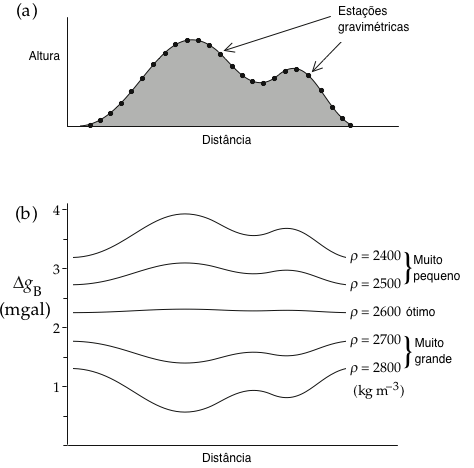
\includegraphics[width=0.6\linewidth]{fig/Fig_02.35} 

}

\caption{Determinação da densidade de rochas próximas à superfície pelo método de Nettleton. (a) Medições de gravidade são feitas em um perfil através de uma pequena colina. (b) Os dados são corrigidos para elevação com vários valores de teste da densidade. A densidade ótima fornece uma correlação mínima entre a anomalia gravitacional $(\Delta g_{B})$ e a topografia.}\label{fig:nettleton}
\end{figure}

Um perfil de estações gravitacionais estreitamente espaçadas é medido através de uma pequena colina (Figura \ref{fig:nettleton}). A correção de elevação combinada é aplicada a cada medição. Suponha que a densidade média real da colina seja \(2600\; \mathrm{kgm}^{-3}\). Se o valor assumido para \(\rho\) for muito pequeno \(\left(\text{digamos}, 2400\; \mathrm{kg} \mathrm{m}^{-3}\right)\), o valor de \(\Delta g_{\mathrm{BP}}\) em cada estação será muito pequeno. A discrepância é proporcional à elevação, então a anomalia da gravidade Bouguer é uma imagem positiva da topografia. Se o valor assumido para \(\rho\) for muito grande \(\left(\text{digamos}, 2800\; \mathrm{kg} \mathrm{m}^{-3}\right)\), a situação oposta ocorre. O muito é subtraído em cada ponto, dando uma anomalia computada que é uma imagem negativa da topografia. O valor ótimo para a densidade é encontrado quando a anomalia da gravidade tem correlação mínima com a topografia.

\hypertarget{anomalias-gravimetricas-ar-livre-free-air-e-bouger}{%
\section{Anomalias gravimétricas ar livre (free-air) e Bouger}\label{anomalias-gravimetricas-ar-livre-free-air-e-bouger}}

Suponha que possamos medir a gravidade no elipsoide de referência. Se a distribuição da densidade dentro da Terra é homogênea, a gravidade medida deve concordar com a gravidade teórica dada pela fórmula da gravidade normal. As correções de gravidade descritas anteriormente compensam a situação usual de que o ponto de medição não está no elipsoide. Uma discrepância entre a gravidade medida corrigida e a gravidade teórica é chamada de anomalia gravitacional. Surge porque a densidade do interior da Terra não é homogênea como se supõe. Os tipos mais comuns de anomalia gravitacional são a \emph{anomalia Bouguer e a anomalia do ar livre (free-air)}.

A anomalia gravimétrica Bouger \(\left(\Delta g_{B}\right)\) é definida pela aplicação de todas as correcções descritas individualmente

\begin{align}
\Delta g_{\mathrm{B}}=g_{\mathrm{m}}+\left(\Delta g_{\mathrm{FA}}-\Delta g_{\mathrm{BP}}+\Delta g_{\mathrm{T}}+\Delta g_{\mathrm{tidc}}\right)-g_{\mathrm{n}}
\label{eq:0248}
\end{align}

Nesta fórmula, \(g_{\mathrm{m}}\) e \(g_{\mathrm{n}}\) são os valores de gravidade medida e gravidade normal; as correções entre parênteses são a correção de ar livre \(\left(\Delta g_{\mathrm{FA}}\right)\), correção da placa Bouguer \(\left(\Delta g_{\mathrm{BP}}\right)\), correção do terreno \(\left(\Delta g_{\mathrm{T}}\right)\) e correção de maré \(\left(\Delta g_{\mathrm{tide}}\right)\).

A anomalia de ar livre \(\left(\Delta g_{\mathrm{F}}\right)\) é definida aplicando-se apenas as correções de ar livre, terreno e maré à gravidade medida:

\begin{align}
\Delta g_{\mathrm{F}}=g_{\mathrm{m}}+\left(\Delta g_{\mathrm{FA}}+\Delta g_{\mathrm{T}}+\Delta g_{\mathrm{tidc}}\right)-g_{\mathrm{n}}
\label{eq:0249}
\end{align}

As anomalias Bouguer e de ar livre na mesma estrutura podem parecer bem diferentes. Considere primeiro o bloco topográfico (representando uma cadeia de montanhas) mostrado na Figura \ref{fig:anomalias}a. Para essa estrutura simples, negligenciamos as correções do terreno e das marés. A diferença entre a anomalia de Bouguer e a anomalia do ar livre surge da correção da placa de Bouguer. No cálculo da anomalia de Bouguer, a elevação simples da estação de medição é levada em conta juntamente com a correção de ar livre. A gravidade medida contém a atração da massa de terra acima do elipsoide, que é compensada com a correção da placa de Bouguer. A estrutura subterrânea não varia lateralmente, portanto a medida corrigida está de acordo com o valor teórico e a anomalia de Bouguer está em toda parte zero ao longo da cadeia montanhosa. Ao computar a anomalia de ar livre, somente a correção de ar livre é aplicada; a parte da gravidade medida devido à atração da massa de terra acima do elipsoide não é levada em consideração. Longe do bloco de montanha, as anomalias de Bouguer e de ar livre são iguais a zero. Sobre a montanha, a massa do bloco de montanha aumenta a gravidade medida em comparação com o valor de referência e resulta em uma anomalia de ar livre positiva em toda a cadeia montanhosa.

\begin{figure}

{\centering 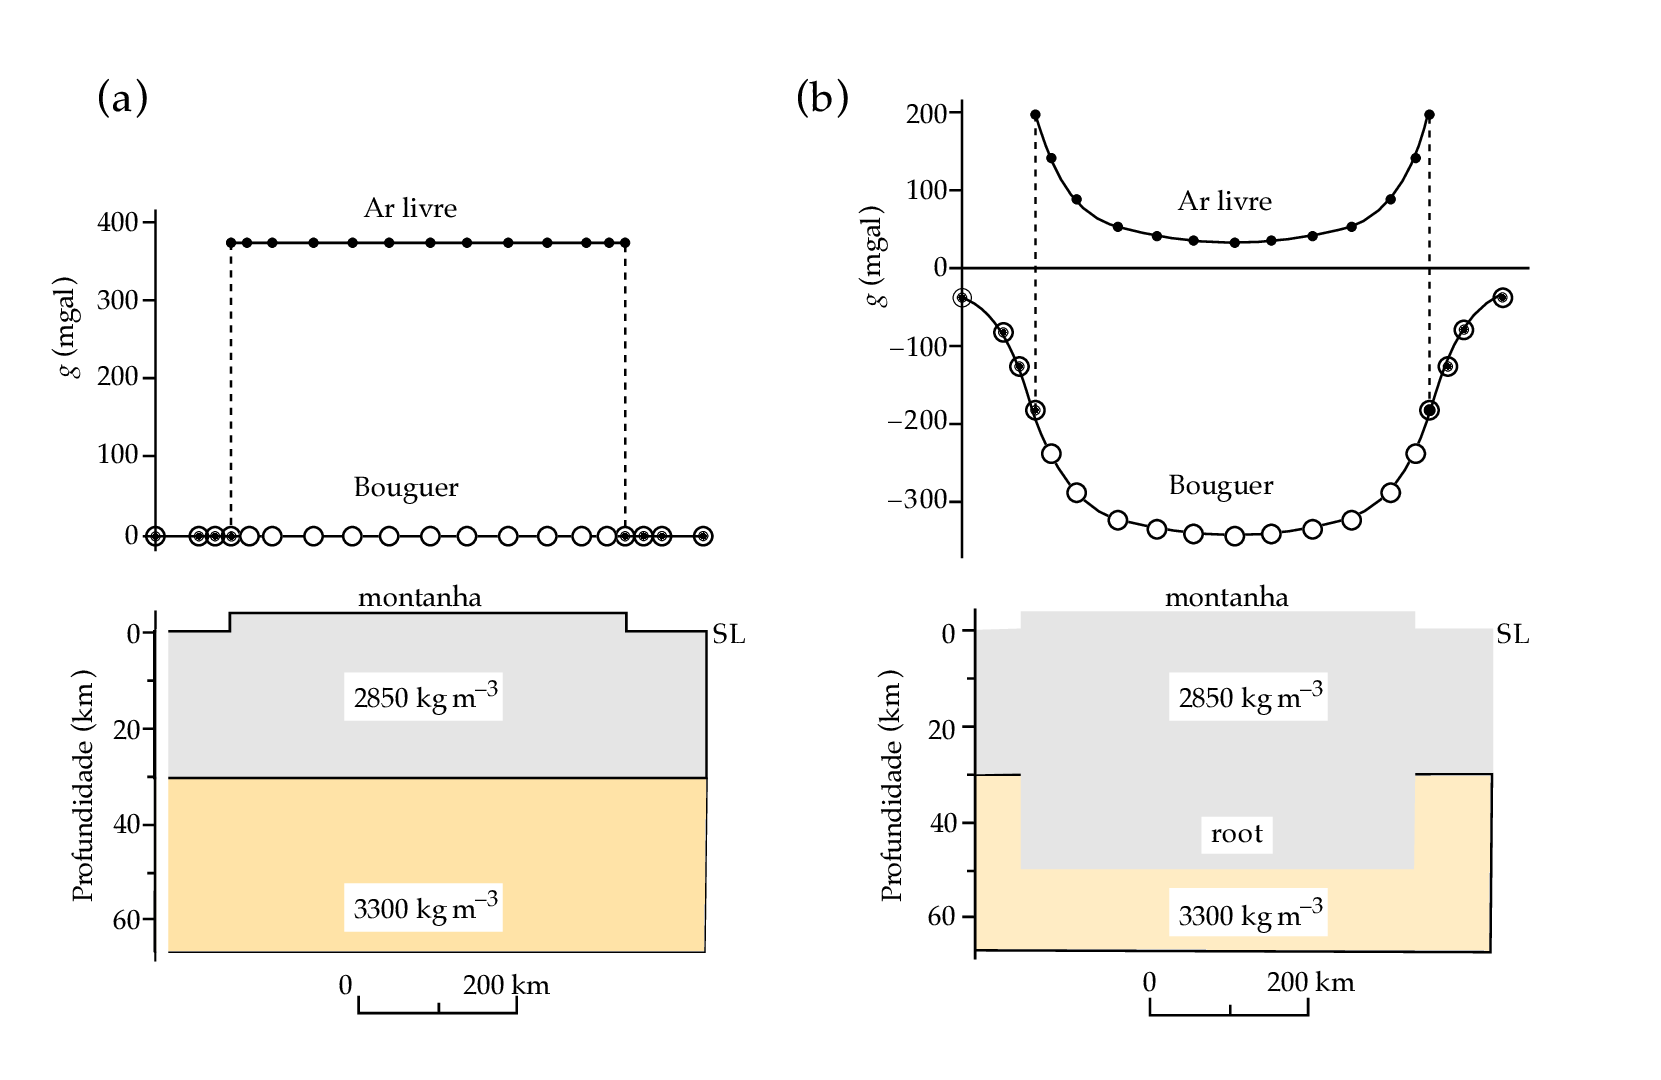
\includegraphics[width=0.8\linewidth]{fig/Fig_02.36} 

}

\caption{Anomalias de ar livre e Bouguer em toda a cordilheira. Em (a) a montanha é modelada por um bloco totalmente suportado, e em (b) a massa da montanha acima do nível do mar (SL) é compensada por uma raiz crustal menos densa, que se projeta para baixo no manto mais denso.}\label{fig:anomalias}
\end{figure}

De fato, dados sísmicos mostram que a crosta terrestre é geralmente muito mais espessa do que o normal sob uma cadeia de montanhas. Isso significa que um bloco de rochas crustais menos densas se projeta no manto mais denso (\ref{fig:anomalias}b). Depois de fazer as correções da placa de ar livre e da Bouguer, permanece uma anomalia de Bouguer devido a um bloco que representa a ``zona das raízes'' da cordilheira. Como isso é menos denso que o manto adjacente e subjacente, constitui um déficit de massa. A atração em um gravímetro nas estações em um perfil através da cordilheira será menor do que na Figura \ref{fig:anomalias}a, então a medida corrigida será menor que o valor de referência. Uma anomalia Bouguer fortemente negativa é observada ao longo do perfil. A certa distância do bloco da montanha, as Bouguer e as anomalias de ar livre são iguais, mas elas não são mais zero, porque a anomalia de Bouguer agora contém o efeito da zona de raiz. Sobre o bloco de montanha, a anomalia de ar livre tem um deslocamento positivo constante da anomalia de Bouguer, como no exemplo anterior. Note que, embora a anomalia de ar livre seja positiva, ela cai para um valor muito baixo sobre o centro do bloco. Neste ponto, a atração da montanha é parcialmente cancelada pela falta de atração da zona de raiz menos densa.

\hypertarget{interpretacao-de-anomalias-gravimetricas}{%
\section{Interpretação de anomalias gravimétricas}\label{interpretacao-de-anomalias-gravimetricas}}

\hypertarget{anomalias-regional-e-residual}{%
\subsection{Anomalias regional e resídual}\label{anomalias-regional-e-residual}}

Uma anomalia gravitacional resulta da distribuição não homogênea da densidade na Terra. Suponha que a densidade de rochas em um corpo subsuperficial seja \(\rho\) e a densidade das rochas ao redor do corpo seja \(\rho_0\). A diferença é chamada de contraste de densidade do corpo em relação às rochas circundantes. Se o corpo tiver uma densidade mais alta que a rocha encaixante, ele terá um contraste de densidade positivo; um corpo com densidade menor que a rocha encaixante tem um contraste de densidade negativo. Sobre um corpo de alta densidade, a gravidade medida é aumentada; após a redução para o elipsoide de referência e a subtração da gravidade normal, uma anomalia gravitacional positiva é obtida. Da mesma forma, uma anomalia negativa ocorre em uma região de baixa densidade. A presença de uma anomalia gravitacional indica um corpo ou estrutura com densidade anômala; o sinal da anomalia é o mesmo do contraste de densidade e mostra se a densidade do corpo é maior ou menor que o normal.

A aparência de uma anomalia gravitacional é afetada pelas dimensões, contraste de densidade e profundidade do corpo anômalo. A extensão horizontal de uma anomalia é frequentemente chamada de seu ``comprimento de onda'' aparente. O comprimento de onda de uma anomalia é uma medida da profundidade da massa anômala. Corpos grandes e profundos dão origem a anomalias amplas (de comprimento de onda longo) e de baixa amplitude, enquanto corpos pequenos e rasos causam anomalias estreitas (de curto comprimento de onda) e agudas.

Normalmente, um mapa de anomalias da gravidade Bouguer contém anomalias sobrepostas de várias fontes. As anomalias de comprimento de onda longo devido a contrastes de densidade profunda são chamadas de anomalias regionais. Eles são importantes para entender a estrutura em larga escala da crosta terrestre sob grandes características geográficas, como cordilheiras, cadeias oceânicas e zonas de subducção. Anomalias residuais de comprimento de onda curto são devidas a massas anômalas superficiais que podem ser de interesse para exploração comercial. O conhecimento geológico é essencial para interpretar as anomalias residuais. Em áreas de escudo erodidas, como o Canadá ou a Escandinávia, anomalias com comprimentos de onda muito curtos podem ser devidas a corpos mineralizados próximos da superfície. Em bacias sedimentares, anomalias de curto ou médio comprimento de onda podem surgir de estruturas relacionadas a reservatórios de petróleo ou gás natural.

\hypertarget{representacao-de-anomalias-regional-e-residual}{%
\subsection{Representação de anomalias regional e resídual}\label{representacao-de-anomalias-regional-e-residual}}

A separação de anomalias de origem regional e local é um passo importante na interpretação de um mapa gravitacional. A análise pode ser baseada em perfis selecionados em alguma estrutura, ou pode envolver a distribuição bidimensional de anomalias em um mapa de gravidade. Diversas técnicas foram aplicadas à decomposição de uma anomalia gravitacional em suas partes constituintes. Eles variam em sofisticação, desde a simples inspeção visual do padrão de anomalia até a análise matemática avançada. Alguns exemplos desses métodos são descritos abaixo.

\hypertarget{analise-visual}{%
\subsubsection{Análise visual}\label{analise-visual}}

A maneira mais simples de representar a anomalia regional em um perfil de gravidade é ajustando visualmente a tendência de larga escala com uma curva suave (Figura \ref{fig:anoreg}). O valor da gravidade regional dado por esta tendência é subtraído ponto a ponto da anomalia da gravidade Bouguer. Esse método permite que o intérprete se ajuste a curvas que deixam anomalias residuais com um sinal

\begin{figure}

{\centering 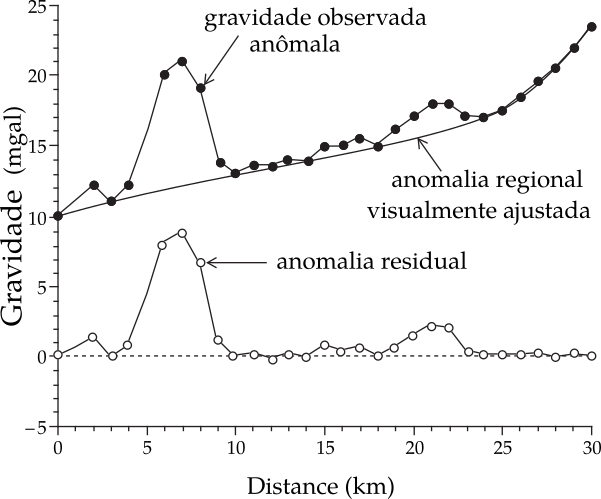
\includegraphics[width=0.8\linewidth]{fig/Fig_02.37} 

}

\caption{Representação da anomalia regional em um perfil de gravidade ajustando visualmente a tendência em grande escala com uma curva suave.}\label{fig:anoreg}
\end{figure}

Esta abordagem pode ser adaptada para a análise de um mapa de gravidade, suavizando visualmente as linhas de contorno. Na Figura \ref{fig:anomapa}a, as linhas de contorno da curva de gravidade Bouguer são bem nítidas em torno de uma anormalidade local. Os contornos mais suavemente curvos foram continuados suavemente como linhas pontilhadas. Eles indicam como o intérprete pensa que o campo gravitacional (Figura \ref{fig:anomapa}b) continuaria na ausência da anormalidade local. Os valores da gravidade Bouguer regional e original são interpolados dos mapas correspondentes em pontos espaçados em uma grade regular. O valor regional é subtraído da anomalia de Bouguer em cada ponto e os resíduos calculados são contornados para dar um mapa da anomalia da gravidade local (Figura \ref{fig:anomapa}c). A experiência e habilidade do intérprete são fatores importantes no sucesso dos métodos visuais.

\begin{figure}

{\centering 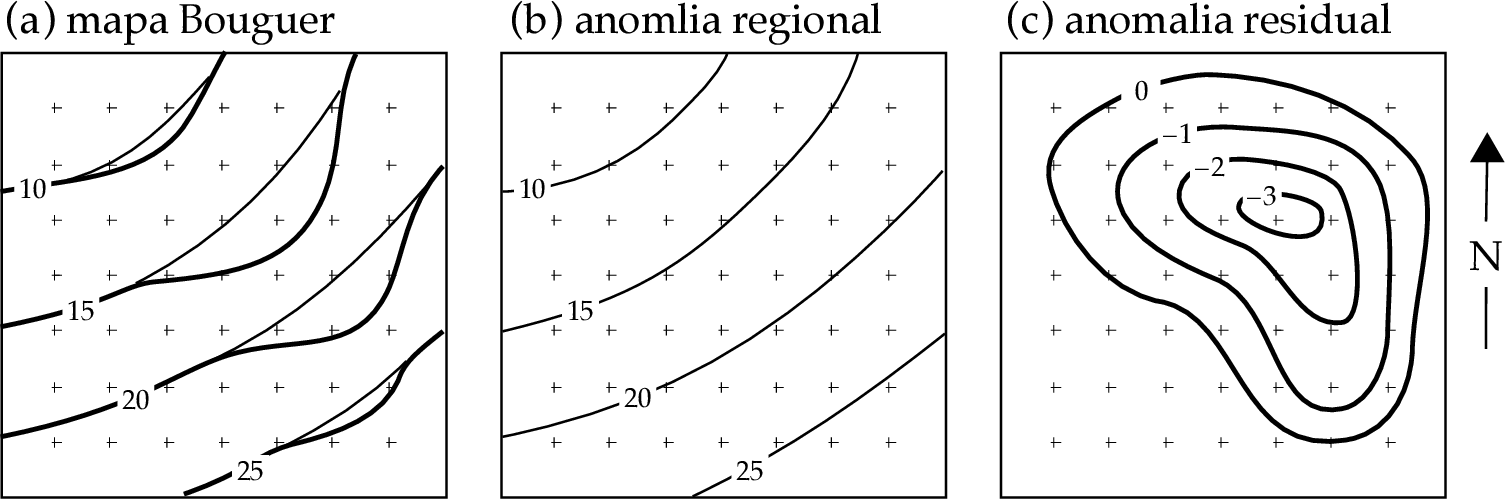
\includegraphics[width=0.8\linewidth]{fig/Fig_02.38} 

}

\caption{Remoção de tendência regional de um mapa de gravidade por suavidade de contorno: (a) suavidade manual de contorno das linhas sobre o mapa original de Bouguer, (b) mapa da variação da gravidade regional, (c) anomalia da gravidade residual após subtrair a variação regional do mapa da gravidade de Bouguer. Os valores estão em mgal.}\label{fig:anomapa}
\end{figure}

\hypertarget{representacao-polinomial}{%
\subsubsection{Representação polinomial}\label{representacao-polinomial}}

Em um método alternativo, a tendência regional é representada por uma linha reta ou, mais geralmente, por uma curva polinomial lisa. Se \(x\) denota a posição horizontal em um perfil de gravidade, a gravidade regional \(\Delta g_\mathrm{R}\) pode ser escrita

\begin{align}
\Delta g_\mathrm{R}=\Delta g_0 + \Delta g_1 x +\Delta g_2 x^2 +\Delta g_3x^3 + \cdots + \Delta g_n x^n   \label{eq:0250}
\end{align}

O polinômio é ajustado pelo método dos mínimos quadrados ao perfil de gravidade observado. Isto dá valores ótimos para os coeficientes \(\Delta g_n\). O método também tem desvantagens. Quanto maior a ordem do polinômio, melhor se ajusta às observações (Figura \ref{fig:anopoli}). O extremo ridículo é quando a ordem do polinômio é um a menos que o número de observações; a curva então passa perfeitamente por todos os pontos de dados, mas a anomalia da gravidade regional não tem significado geológico. O julgamento do intérprete é importante na seleção da ordem do polinômio, que geralmente é escolhido para ser a menor ordem possível que represente a maior parte da tendência regional.
Além disso, uma curva ajustada por mínimos quadrados deve passar pela média dos valores de gravidade, de modo que as anomalias residuais sejam divididas igualmente entre valores positivos e negativos. Cada anomalia residual é flanqueada por anomalias de sinais opostos (Figura \ref{fig:anopoli}), que são devidas à mesma massa anômala que causou a anomalia central e, portanto, não têm significado próprio.

\begin{figure}

{\centering 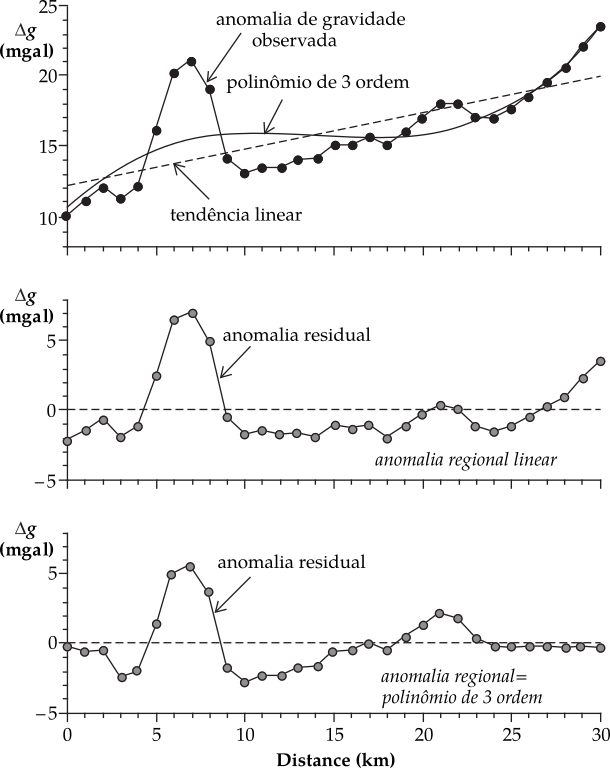
\includegraphics[width=0.8\linewidth]{fig/Fig_02.39} 

}

\caption{Representação da tendência regional por uma curva polinomial suave ajustada ao perfil de gravidade observado pelo método dos mínimos quadrados.}\label{fig:anopoli}
\end{figure}

Ajuste polinomial também pode ser aplicado a mapas de gravidade. Assume-se que a anomalia regional pode ser representada por uma superfície lisa, \(\Delta g(x, y)\), que é um polinômio de baixa ordem das coordenadas de posição horizontal \(x\) e \(y\). No caso mais simples, a anomalia regional é expressada como um polinômio de primeira ordem, ou plano. Para expressar mudanças no gradiente da gravidade, é necessário um polinômio de ordem superior. Por exemplo, a gravidade regional dada por um polinômio de segunda ordem é escrita

\begin{align}
\Delta g(x,y) &= \Delta g_0 + \Delta g_{x1} x + \Delta g_{y1} y\\
& +\Delta g_{x2} x^2 +\Delta g_{y2} y^2 ++\Delta g_{xy} xy. \label{eq:0251}
\end{align}

Como na análise do perfil, os valores ótimos dos coeficientes \(\Delta g_{x1}\), \(\Delta g_{y1}\), etc., são determinados por ajuste por mínimos quadrados. A anomalia residual é novamente computada ponto a ponto pela subtração da regional do dado original

\hypertarget{representacao-por-series-de-fourier}{%
\subsubsection{Representação por séries de Fourier}\label{representacao-por-series-de-fourier}}

A anomalia gravitacional ao longo de um perfil pode ser analisada com técnicas desenvolvidas para investigar séries temporais. Em vez de variar com o tempo, como o sinal sísmico faz em um sismógrafo, a anomalia gravitacional \(\Delta g (x)\) varia de acordo com a posição \(x\) ao longo do perfil. Para uma distribuição espacial, o número da onda, \(k= 2\pi / \lambda\), é a contrapartida da frequência de uma série temporal. Se for possível supor que sua variação é periódica, a função \(\Delta g (x)\) pode ser expressa como a soma de uma série de harmônicos discretas. Cada harmônico é uma função \(\mathrm{seno}\) ou \(\mathrm{cosseno}\) cujo argumento é um múltiplo do número da onda fundamental. A expressão para \(\Delta g(x)\) é chamada de uma série de Fourier.

A decomposição de uma anomalia complexa (ou série temporal) em termos de variações periódicas mais simples de diferentes comprimentos de onda é chamada análise de Fourier e é um método poderoso para resolver as componentes mais importantes do sinal original.

A variação bidimensional de uma anomalia gravitacional mapeada pode ser expressa de maneira semelhante com o auxílio de \textbf{séries duplas de Fourier}. Como no caso unidimensional mais simples de uma anomalia gravitacional em um perfil, a expressão de anomalias gravimétricas bidimensionais por duas séries de Fourier é análoga à soma das funções senoidais ponderadas. Estes podem ser visualizados como corrugações do plano de \(xy\) (Figura \ref{fig:anofourier}), com cada ondulação ponderada de acordo com sua importância para \(\Delta g (x, y)\).

\begin{figure}

{\centering 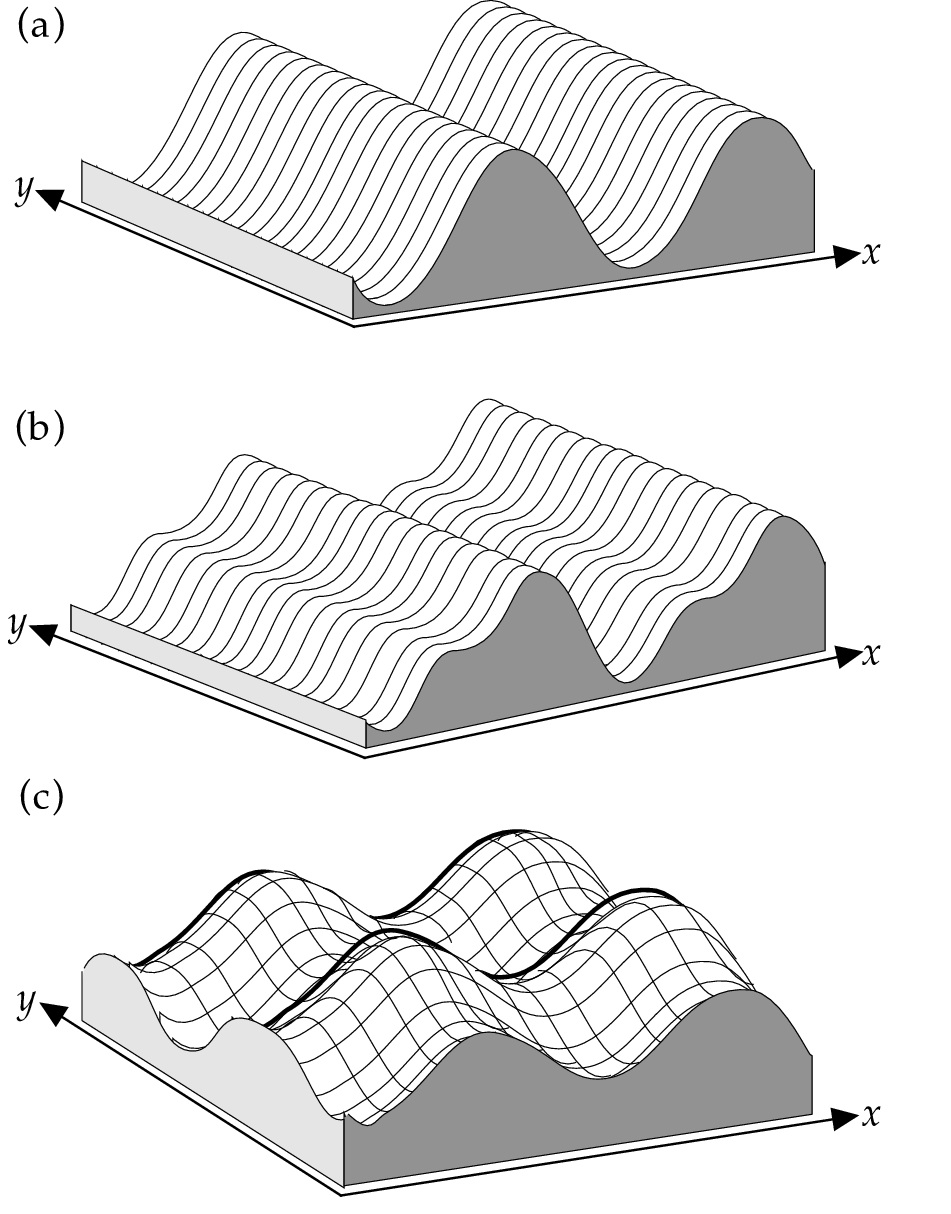
\includegraphics[width=0.8\linewidth]{fig/Fig_02.40} 

}

\caption{Expressão da variação bidimensional de uma anomalia gravitacional usando duas séries de Fourier: (a) um único harmônico na direção $x$, (b) dois harmônicos na direção $x$, (c) harmônicos únicos sobrepostos nas coordenadas $x$ e $y$ direções, respectivamente (depois de Davis, 1973).}\label{fig:anofourier}
\end{figure}

\hypertarget{aprimoramento-e-filtragem-de-anomalias}{%
\subsubsection{Aprimoramento e filtragem de anomalias}\label{aprimoramento-e-filtragem-de-anomalias}}

A discussão acima mostra como uma função que é periódica pode ser expressa como uma somade harmônicos de Fourier de um comprimento de onda fundamental. Ao dividir o sinal observado em componentes discretos, é possível remover alguns deles e reconstruir uma versão filtrada da anomalia original. No entanto, os requisitos de comportamento periódico e discrição do conteúdo harmônico geralmente não são atendidos. Por exemplo, a variação da gravidade de um ponto para outro geralmente não é periódica. Além disso, se o conteúdo harmônico de uma função é composto de múltiplos distintos de uma frequência fundamental ou número de onda, o espectro de comprimento de onda consiste em um número de valores distintos. No entanto, muitas funções de interesse geofísico são melhor representadas por um espectro contínuo de comprimentos de onda.

Para lidar com esse tipo de problema, a variação espacial da gravidade é representada por uma integral de Fourier, que consiste em um conjunto contínuo de frequências ou números de onda, em vez de um conjunto discreto. A integral de Fourier pode ser usada para representar funções não periódicas. Ele usa números complexos, que são números que envolvem \(i\), a raiz quadrada de \(-1\). Se a anomalia da gravidade é analisada em duas dimensões (em vez de em um único perfil), uma integral bidimensional é necessário, análogo à representação da série dupla de Fourier. A gravidade observada pode então ser manipulada usando as técnicas de transformada de Fourier. Essas técnicas envolvem cálculos intensivos e são ideais para o processamento de dados digitais com computadores poderosos.

A transformada bidimensional de Fourier de um mapa gravitacional permite filtrar digitalmente as anomalias da gravidade. Um filtro é uma função espacial das coordenadas \(x\) e \(y\). Quando a função \(\Delta G (x, y)\) representando os dados da gravidade é multiplicada pela função do filtro, uma nova função é produzida. O processo é chamado de convolução e a saída é um mapa dos dados de gravidade filtrados. O cálculo no domínio espacial definido pelas coordenadas \(x\) e \(y\) pode ser demorado. Geralmente, é mais rápido calcular as transformadas de Fourier das funções de gravidade e filtro, multiplicá-las juntas no domínio de Fourier e, em seguida, realizar uma transformação inversa de Fourier no produto para convertê-lo de volta ao domínio espacial.

A natureza do filtro aplicado no domínio de Fourier pode ser escolhida para eliminar certos comprimentos de onda. Por exemplo, ele pode ser projetado para cortar todos os comprimentos de onda mais curtos do que um comprimento de onda selecionado e para passar comprimentos de onda maiores. Isso é chamado de filtro \emph{passa-baixa}; Ele passa comprimentos de onda longos que têm números baixos de onda. As irregularidades em um mapa de anomalia gravitacional Bouguer (Figura \ref{fig:mapafilter}a) são removidas por filtragem \emph{passa-baixa}, deixando um mapa filtrado (Figura \ref{fig:mapafilter}b) muito mais suave do que o original. Alternativamente, o filtro no domínio de Fourier pode ser projetado para eliminar comprimentos de onda maiores que um comprimento de onda selecionado e para passar comprimentos de onda menores. A aplicação de tal filtro \emph{passa-alta} aumenta o componente de comprimento de onda curto (alto número de ondas) do mapa de gravidade (Figura \ref{fig:mapafilter}c).

\begin{figure}

{\centering 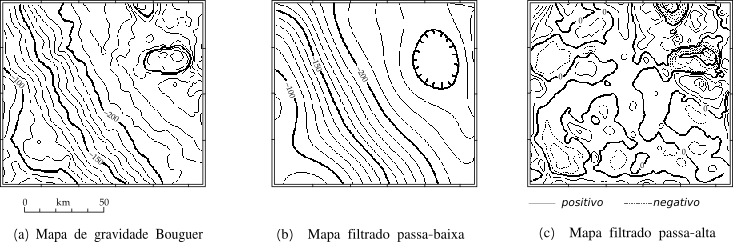
\includegraphics[width=0.9\linewidth]{fig/Fig_02.41} 

}

\caption{O uso da filtragem de comprimento de onda para enfatizar anomalias selecionadas na Sierra Nevada, Califórnia: (a) mapa de gravidade Bouguer não filtrado, (b) mapa de gravidade filtrado de passa-baixa com anomalias regionais de comprimento de onda longo e (c) mapa de gravidade filtrado de passa-alta realçando anomalias locais de curto comprimento de onda. Intervalo de contorno: (a) e (b) 10 mgal, (c) 5 mgal (após Dobrin e Savit, 1988).}\label{fig:mapafilter}
\end{figure}

A filtragem de comprimento de onda pode ser usada para enfatizar anomalias selecionadas. Por exemplo, ao estudar a estrutura crustal em grande escala, as anomalias da gravidade devidas a pequenos corpos locais são de menor interesse que as anomalias regionais, que podem ser melhoradas pela aplicação de um filtro \emph{passa-baixa}. Por outro lado, na investigação de anomalias devido a fontes superficiais da crosta terrestre, o efeito regional pode ser suprimido por filtragem \emph{passa-alta}.

\hypertarget{modelagem-de-anomalias-gravimetricas}{%
\subsubsection{Modelagem de anomalias gravimétricas}\label{modelagem-de-anomalias-gravimetricas}}

Após a remoção dos efeitos regionais, a anomalia da gravidade residual deve ser interpretada em termos de uma distribuição de densidade anômala. Análises modernas são baseadas em modelagem iterativa usando computadores de alta velocidade. Métodos anteriores de interpretação utilizaram a comparação das anomalias da gravidade observadas com as anomalias computadas das formas geométricas. O sucesso dessa abordagem simples é devido à insensibilidade da forma de uma anomalia gravitacional a pequenas variações na distribuição da densidade anômala. Alguns problemas fundamentais da interpretação de anomalias gravitacionais podem ser aprendidos a partir dos efeitos computados dos modelos geométricos. Em particular, é importante perceber que a interpretação das anomalias da gravidade não é única; distribuições de densidade diferentes podem dar a mesma anomalia.

\hypertarget{esfera-uniforme-modelo-para-um-diapiro}{%
\paragraph{Esfera uniforme: modelo para um diapiro}\label{esfera-uniforme-modelo-para-um-diapiro}}

Estruturas diapíricas introduzem material de densidade diferente na rocha encaixante. Um domo de sal de baixa densidade \(\left(\rho=2150\; \mathrm{kg}\, \mathrm{m}^{-3}\right)\) que invade rochas de carbonato de densidade mais alta\(\left(\rho_0=2500\; \mathrm{kg} \mathrm{m}^{-3}\right)\) tem um contraste de densidade de \(\Delta \rho=-350\; \mathrm{kg}\,\mathrm{m}^{-3}\) e causa uma anomalia de gravidade negativa. Um tampão vulcânico \(\left(\rho=2800\; \mathrm{kg}\, \mathrm{m}^{-3}\right)\) que invade um corpo de granito \(\left(\rho_{0}=2600\; \mathrm{kg}\,\mathrm{m}^{-3}\right)\) tem um contraste de densidade de \(\Delta \rho=+200 \,\mathrm{kg}\,\mathrm{m}^{-3}\), o que causa uma anomalia de gravidade positiva. As linhas de contorno em um mapa da anomalia são centralizadas no diapiro, então todos os perfis no centro da estrutura são equivalentes. O corpo anômalo pode ser modelado igualmente por um cilindro vertical ou por uma esfera, que nós iremos avaliar aqui por causa da simplicidade do modelo

Assumindo uma esfera de raio \(R\) e densidade de contraste \(\Delta\rho\) com seu centro na profundidade \(z\) abaixo da superfície (Figura \ref{fig:esferas}). A atração \(\Delta g\) da esfera é como se a massa anômala \(M\) da esfera estivesse concentrada em seu centro. Se medirmos a posição horizontal a partir de um ponto acima do seu centro, à distância \(x\), a componente vertical \(\Delta g_z\) é dado por

\begin{figure}

{\centering 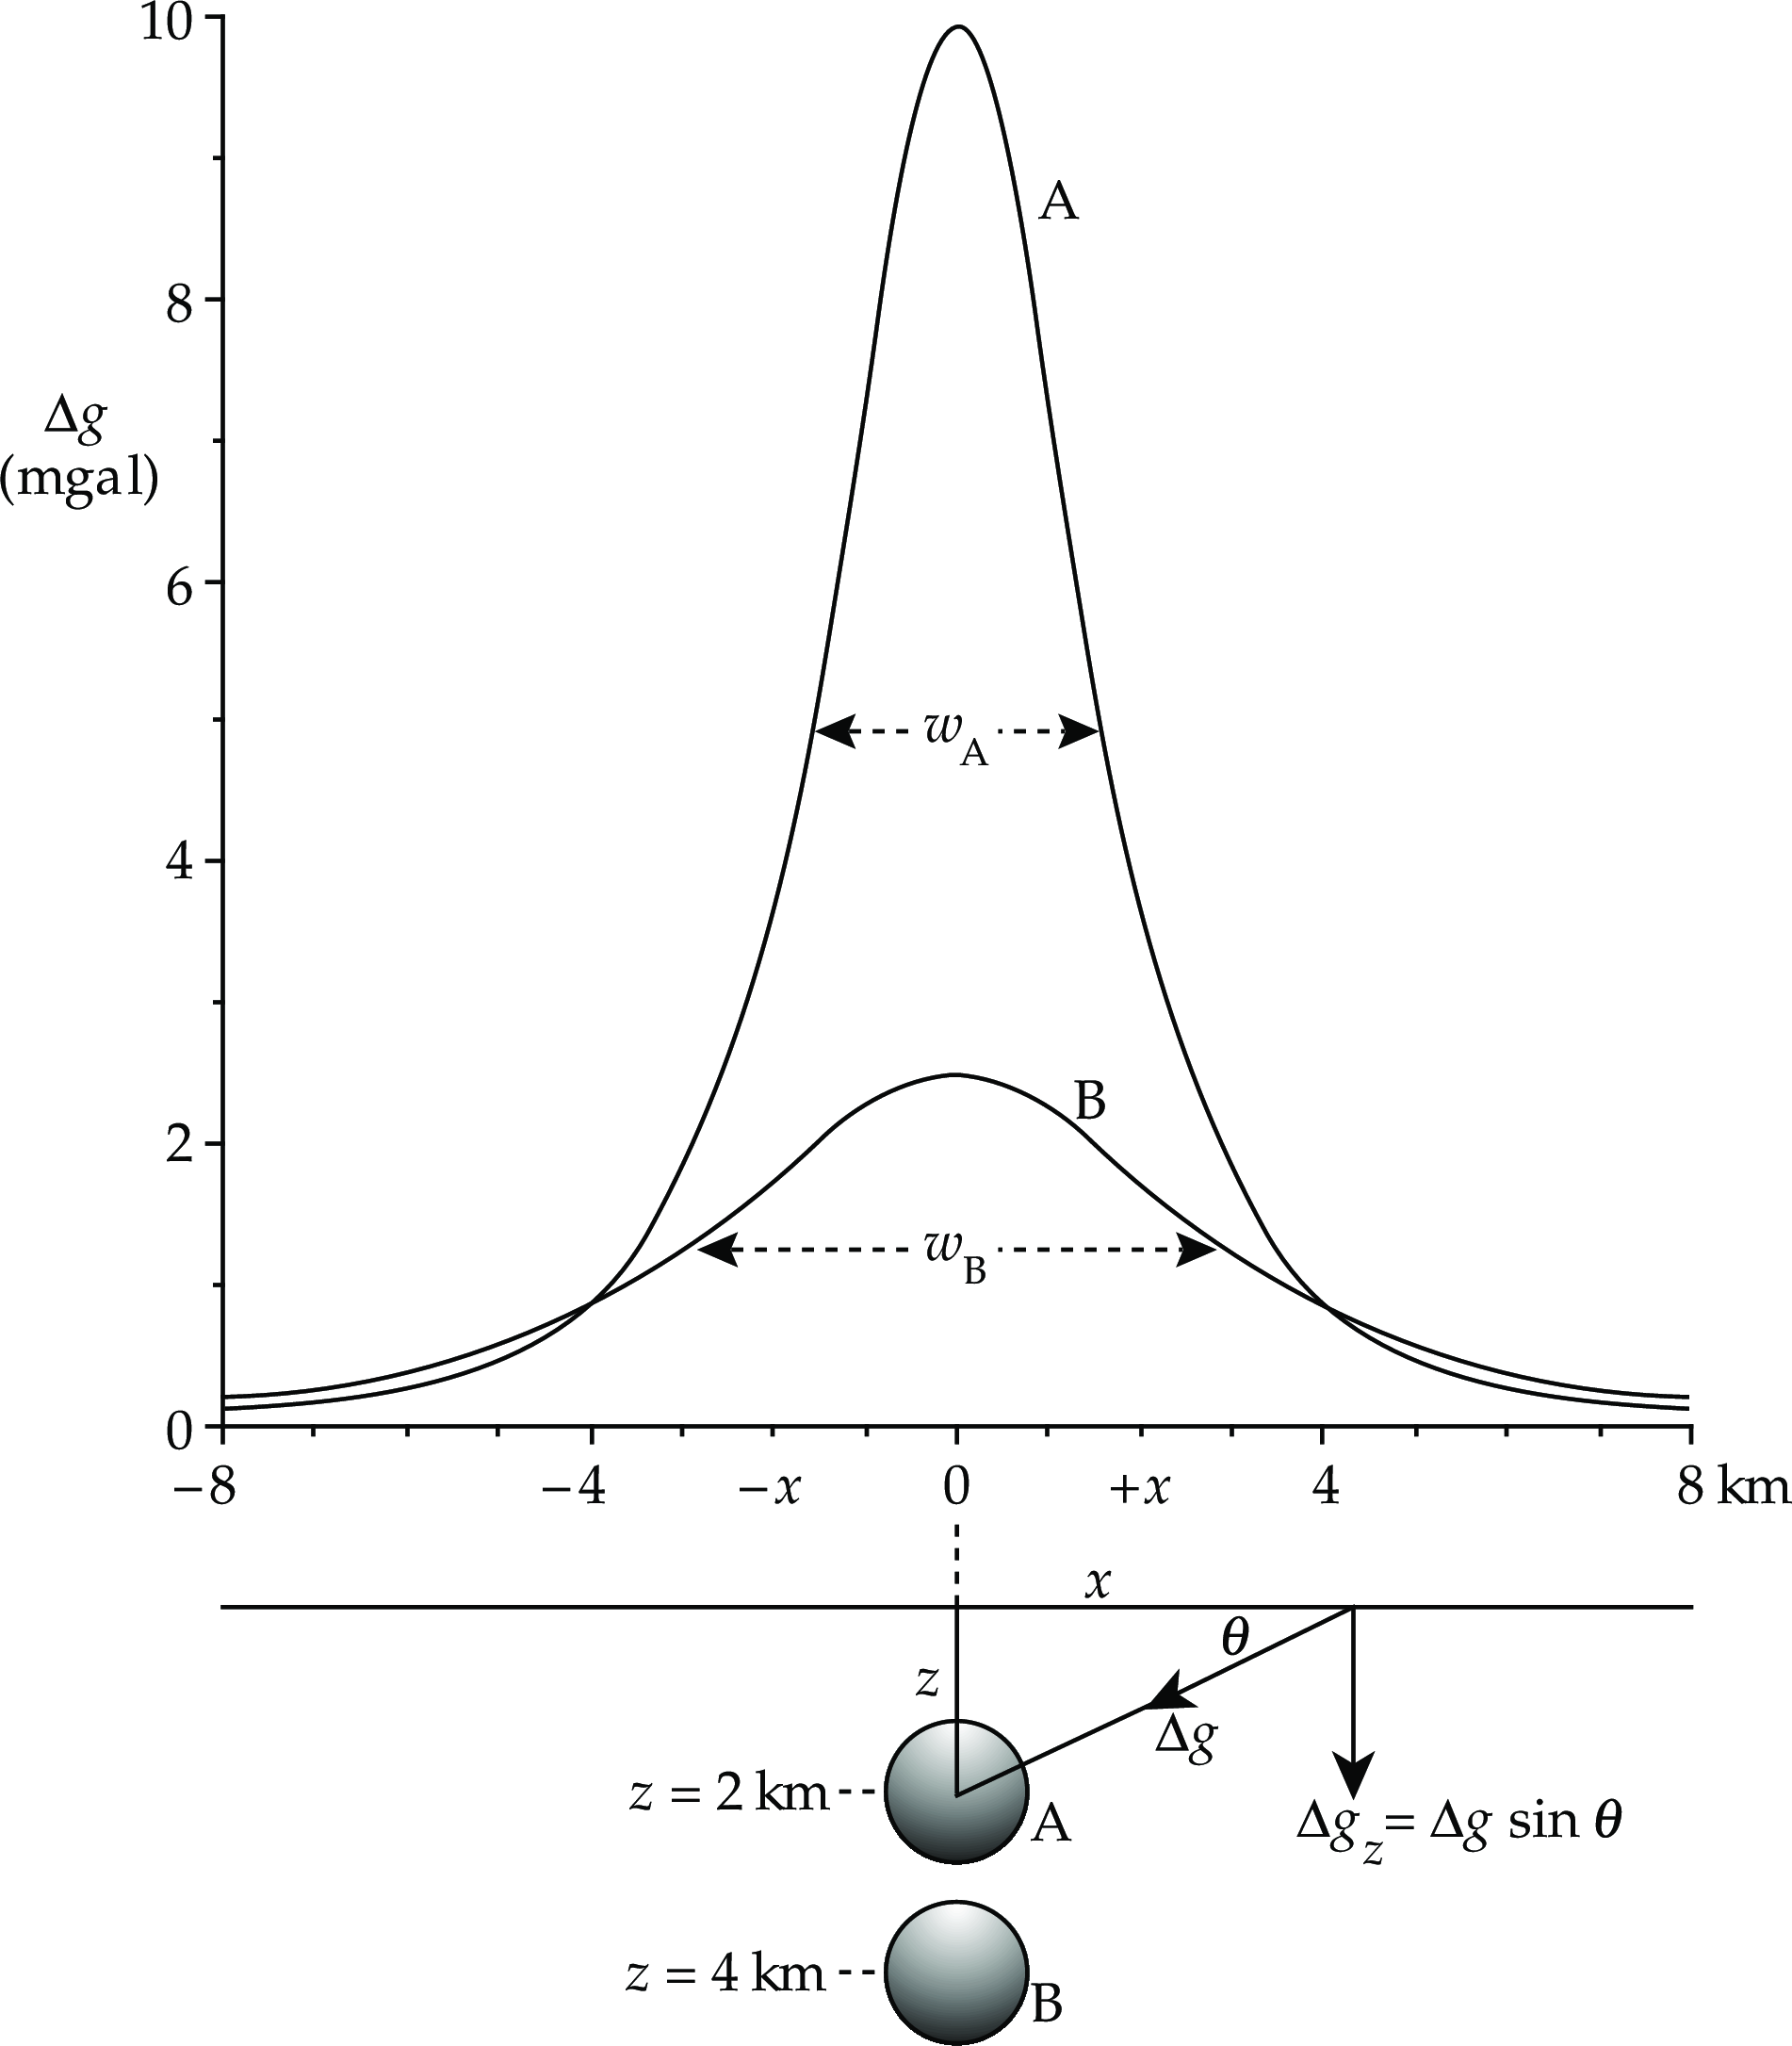
\includegraphics[width=0.6\linewidth]{fig/Fig_02.42} 

}

\caption{Anomalias de gravidade para esferas enterradas com o mesmo raio $R$ e contraste de densidade $\Delta \rho$ mas com seus centros em diferentes profundidades $z$ abaixo da superfície. A anomalia da esfera mais profunda $B$ é mais plana e mais larga que a anomalia da esfera menor $A$.}\label{fig:esferas}
\end{figure}

\begin{equation}
\Delta g_{z}=\Delta g \sin \theta=G \frac{M}{r^{2}} \frac{z}{r}  \label{eq:0252}
\end{equation}

onde

\[ M=\frac{4}{3} \pi R^{3} \Delta \rho \quad \text { e } \quad r^{2}=z^{2}+x^{2}\]

Substituindo estas expressões na Equção \eqref{eq:0252} e reorganizando os termos

\begin{equation}
\begin{aligned} \Delta g_{z} &=\frac{4}{3} \pi G \Delta \rho R^{3} \frac{z}{\left(z^{2}+x^{2}\right)^{3 / 2}} \\ &=\frac{4}{3} \pi G\left(\frac{\Delta \rho R^{3}}{z^{2}}\right)\left[\frac{1}{\left(1+(x / z)^{2}\right)}\right]^{3 / 2} \end{aligned} \label{eq:0253}
\end{equation}

Os termos no primeiro par de parênteses dependem do tamanho, profundidade e densidade do contraste da esfera anômala. Eles determinam a amplitude máxima da anomalia, \(\Delta g_0\), que é alcançada sobre o centro da esfera em \(x=0\). O valor de pico é dado por

\begin{equation}
\Delta g_{0}=\frac{4}{3} \pi G\left(\frac{\Delta \rho R^{3}}{z^{2}}\right) \label{eq:0254}
\end{equation}

Esta equação mostra como a profundidade ao centro da esfera afeta a amplitude de pico da anomalia; quanto maior a profundidade do centro, menor a amplitude (Figura \ref{fig:esferas}). Para uma dada profundidade, a mesma anomalia de pico pode ser produzida por numerosas combinações de \(\Delta \rho\) e \(R\); uma esfera grande com um contraste de baixa densidade pode fornecer uma anomalia idêntica a uma pequena esfera com um contraste de alta densidade. Os dados gravimétricos, por si só, não nos permitem resolver essa ambiguidade.

Os termos do segundo par de parênteses na Equação. \eqref{eq:0253} descrevem como a amplitude da anomalia varia com a distância ao longo do perfil. A anomalia é simétrica em relação a \(x\), atinge um valor máximo \(\Delta g_0\) sobre o centro da esfera \((x=0)\) e diminui para zero a grandes distâncias \((x=\infty)\). Note que quanto maior a profundidade \(z\), mais lentamente a amplitude diminui lateralmente com o aumento de \(x\). Uma fonte profunda produz uma anomalia menor mas mais ampla do que a mesma fonte a uma profundidade menor. A largura \(w\) da anomalia, onde a amplitude tem metade do seu valor máximo, é chamada de ``largura de meia altura''. A profundidade \(z\) para o centro da esfera é deduzida dessa largura de anomalia a partir da relação \(z=0.652w\).

\hypertarget{elemento-de-linha-horizontal}{%
\paragraph{Elemento de linha horizontal}\label{elemento-de-linha-horizontal}}

Muitas estruturas geologicamente interessantes se estendem a grandes distâncias em uma direção, mas têm a mesma forma de seção transversal ao longo da trajetória da estrutura. Se o comprimento ao longo da direção fosse infinito, a variação bidimensional da densidade na área da seção transversal seria suficiente para modelar a estrutura. No entanto, isso não é realmente válido, pois a extensão lateral nunca é infinita. Como regra geral, se o comprimento da estrutura normal ao perfil for maior que vinte vezes sua largura ou profundidade, ela pode ser tratada como bidimensional (2D). Caso contrário, os efeitos finais devido à extensão lateral limitada da estrutura devem ser levados em conta no cálculo de sua anomalia. Um corpo alongado que requer correções finais é por vezes referido como uma estrutura 2.5D. Por exemplo, a distribuição de massa sob corpos alongados como anticlinais, sinclinais e falhas deve ser modelada como estruturas 2.5D. Aqui, vamos lidar com os modelos bidimensionais mais simples dessas estruturas.

Seja uma distribuição de massa linear infinitamente longa com massa \(m\) por unidade de comprimento que se estenda horizontalmente ao longo do eixo \(y\) na profundidade \(z\) (Figura \ref{fig:linha}). A contribuição \(d(\Delta g_z)\) para a anomalia da gravidade vertical \(\Delta g_z\) em um ponto no eixo \(x\) devido a um pequeno elemento de comprimento \(dy\) é

\begin{figure}

{\centering 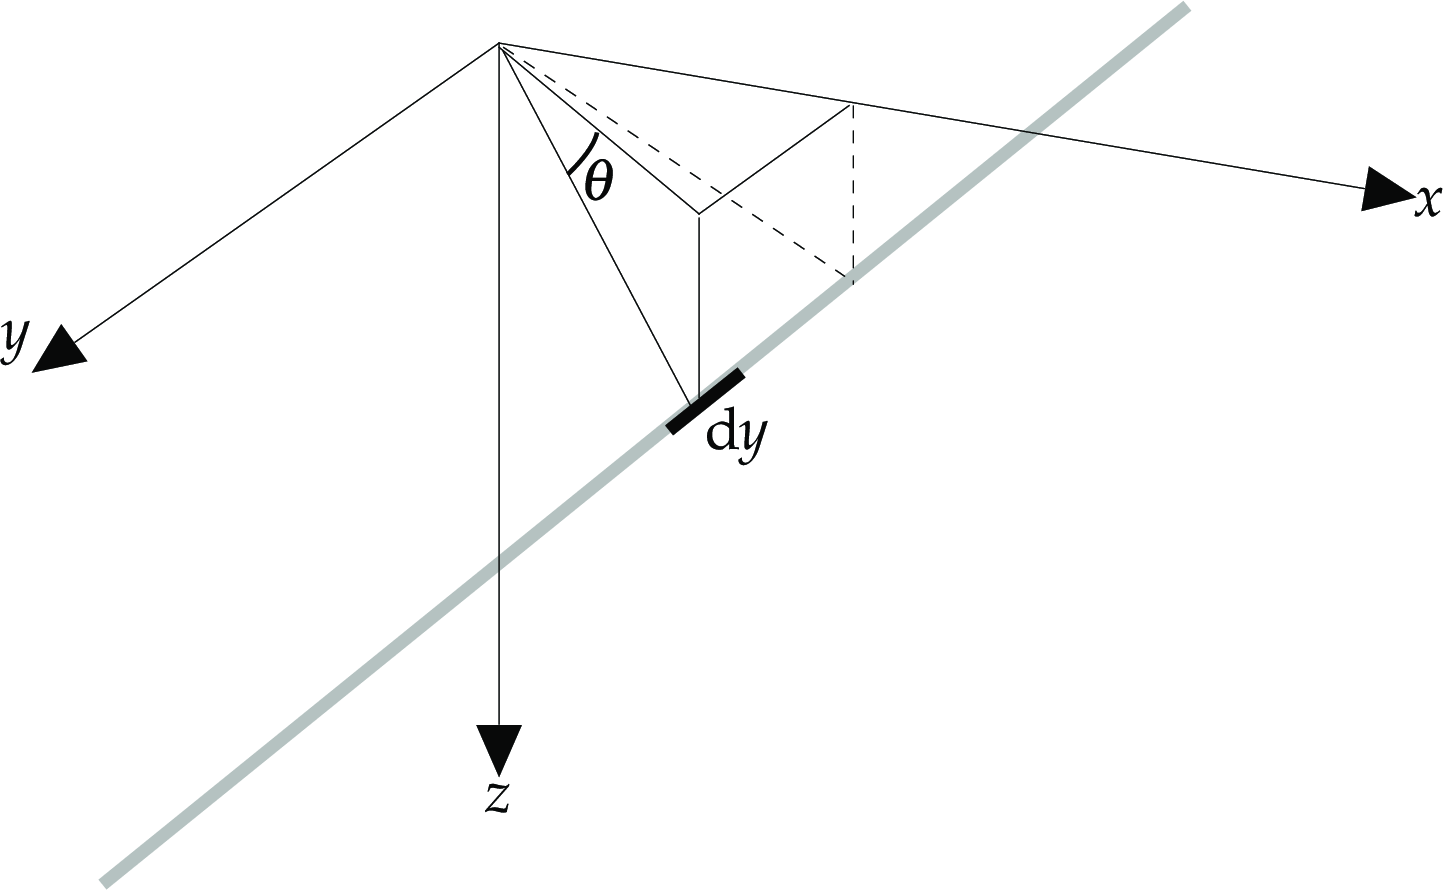
\includegraphics[width=0.6\linewidth]{fig/Fig_02.43} 

}

\caption{Geometria para cálculo da anomalia gravimétrica de uma distribuição de massa linear infinitamente longa com massa $m$ por unidade de comprimento que se estende horizontalmente ao longo do eixo $y$ na profundidade $z$.}\label{fig:linha}
\end{figure}

\begin{equation}
\mathrm{d}\left(\Delta g_{z}\right)=G \frac{m \mathrm{d} y}{r^{2}} \sin \theta=G \frac{m \mathrm{d} y}{r^{2}} \frac{z}{r} \label{eq:0255}
\end{equation}

O elemento de linha se estende ao infinito ao longo dos eixo \(y\) positio e negativo, entaão sua anomalia de gravidade vertical é encontardo pela integração:

\begin{equation}
\Delta g_{z}=G m z \int_{-\infty}^{\infty} \frac{\mathrm{d} y}{r^{3}}=G m z \int_{-\infty}^{\infty} \frac{\mathrm{d} y}{\left(u^{2}+y^{2}\right)^{3 / 2}} \label{eq:0256}
\end{equation}

onde \(u^2=x^2+z^2\). A integração é simplificada pela mudança de variável, tal que \(y=u\,\tan{\varphi}\); então \(dy=u\,\sec^2{\varphi}d\varphi\) e \(\left(u^{2}+y^{2}\right)^{3 / 2}=u^{3} \sec ^{3} \varphi\). Isto dá

\begin{equation}
\Delta g_{z}=\frac{G m z}{u^{2}} \int_{-\pi / 2}^{\pi / 2} \cos \varphi d \varphi  \label{eq:0257}
\end{equation}

que após a avaliação da integral, temos

\begin{equation}
\Delta g_{z}=\frac{2 G m z}{z^{2}+x^{2}}.  \label{eq:0258}
\end{equation}

Esta expressão pode ser escrita como a derivada de uma função potencial \(\Psi\)

\begin{equation}
\Delta g_{z}=G m \frac{2 z}{u^{2}}=-\frac{\partial \Psi}{\partial z} \label{eq:0259}
\end{equation}

\begin{equation}
\Psi=G m \log _{\mathrm{e}}\left(\frac{1}{u}\right)=G m \log _{\mathrm{e}}\left(\frac{1}{\sqrt{x^{2}+z^{2}}}\right) \label{eq:0260}
\end{equation}

\(\Psi\) é chamado de \emph{potencial logarítmico}. As equações \eqref{eq:0258} e \eqref{eq:0260} são resultados úteis para derivar fórmulas para a anomalia gravitacional de estruturas lineares como um anticlinal (ou sinclinal) ou uma falha.

\hypertarget{cilindro-horizontal-modelo-para-anticlinal-e-sinclinal}{%
\paragraph{Cilindro horizontal: modelo para anticlinal e sinclinal}\label{cilindro-horizontal-modelo-para-anticlinal-e-sinclinal}}

A anomalia gravitacional de um anticlinal pode ser modelada assumindo que a dobra ascendente dos estratos trazendo rochas com maior densidade mais próxima da superfície (Figura \ref{fig:cilindro1}a), causando, assim, um contraste de densidade positivo. Um sinclinal é modelado assumindo que seu núcleo é preenchido com camadas de baixa densidade que causam um contraste negativo de densidade. Em cada caso, o modelo geométrico da estrutura é um cilindro horizontal infinito (Figura \ref{fig:cilindro1}b).

\begin{figure}

{\centering 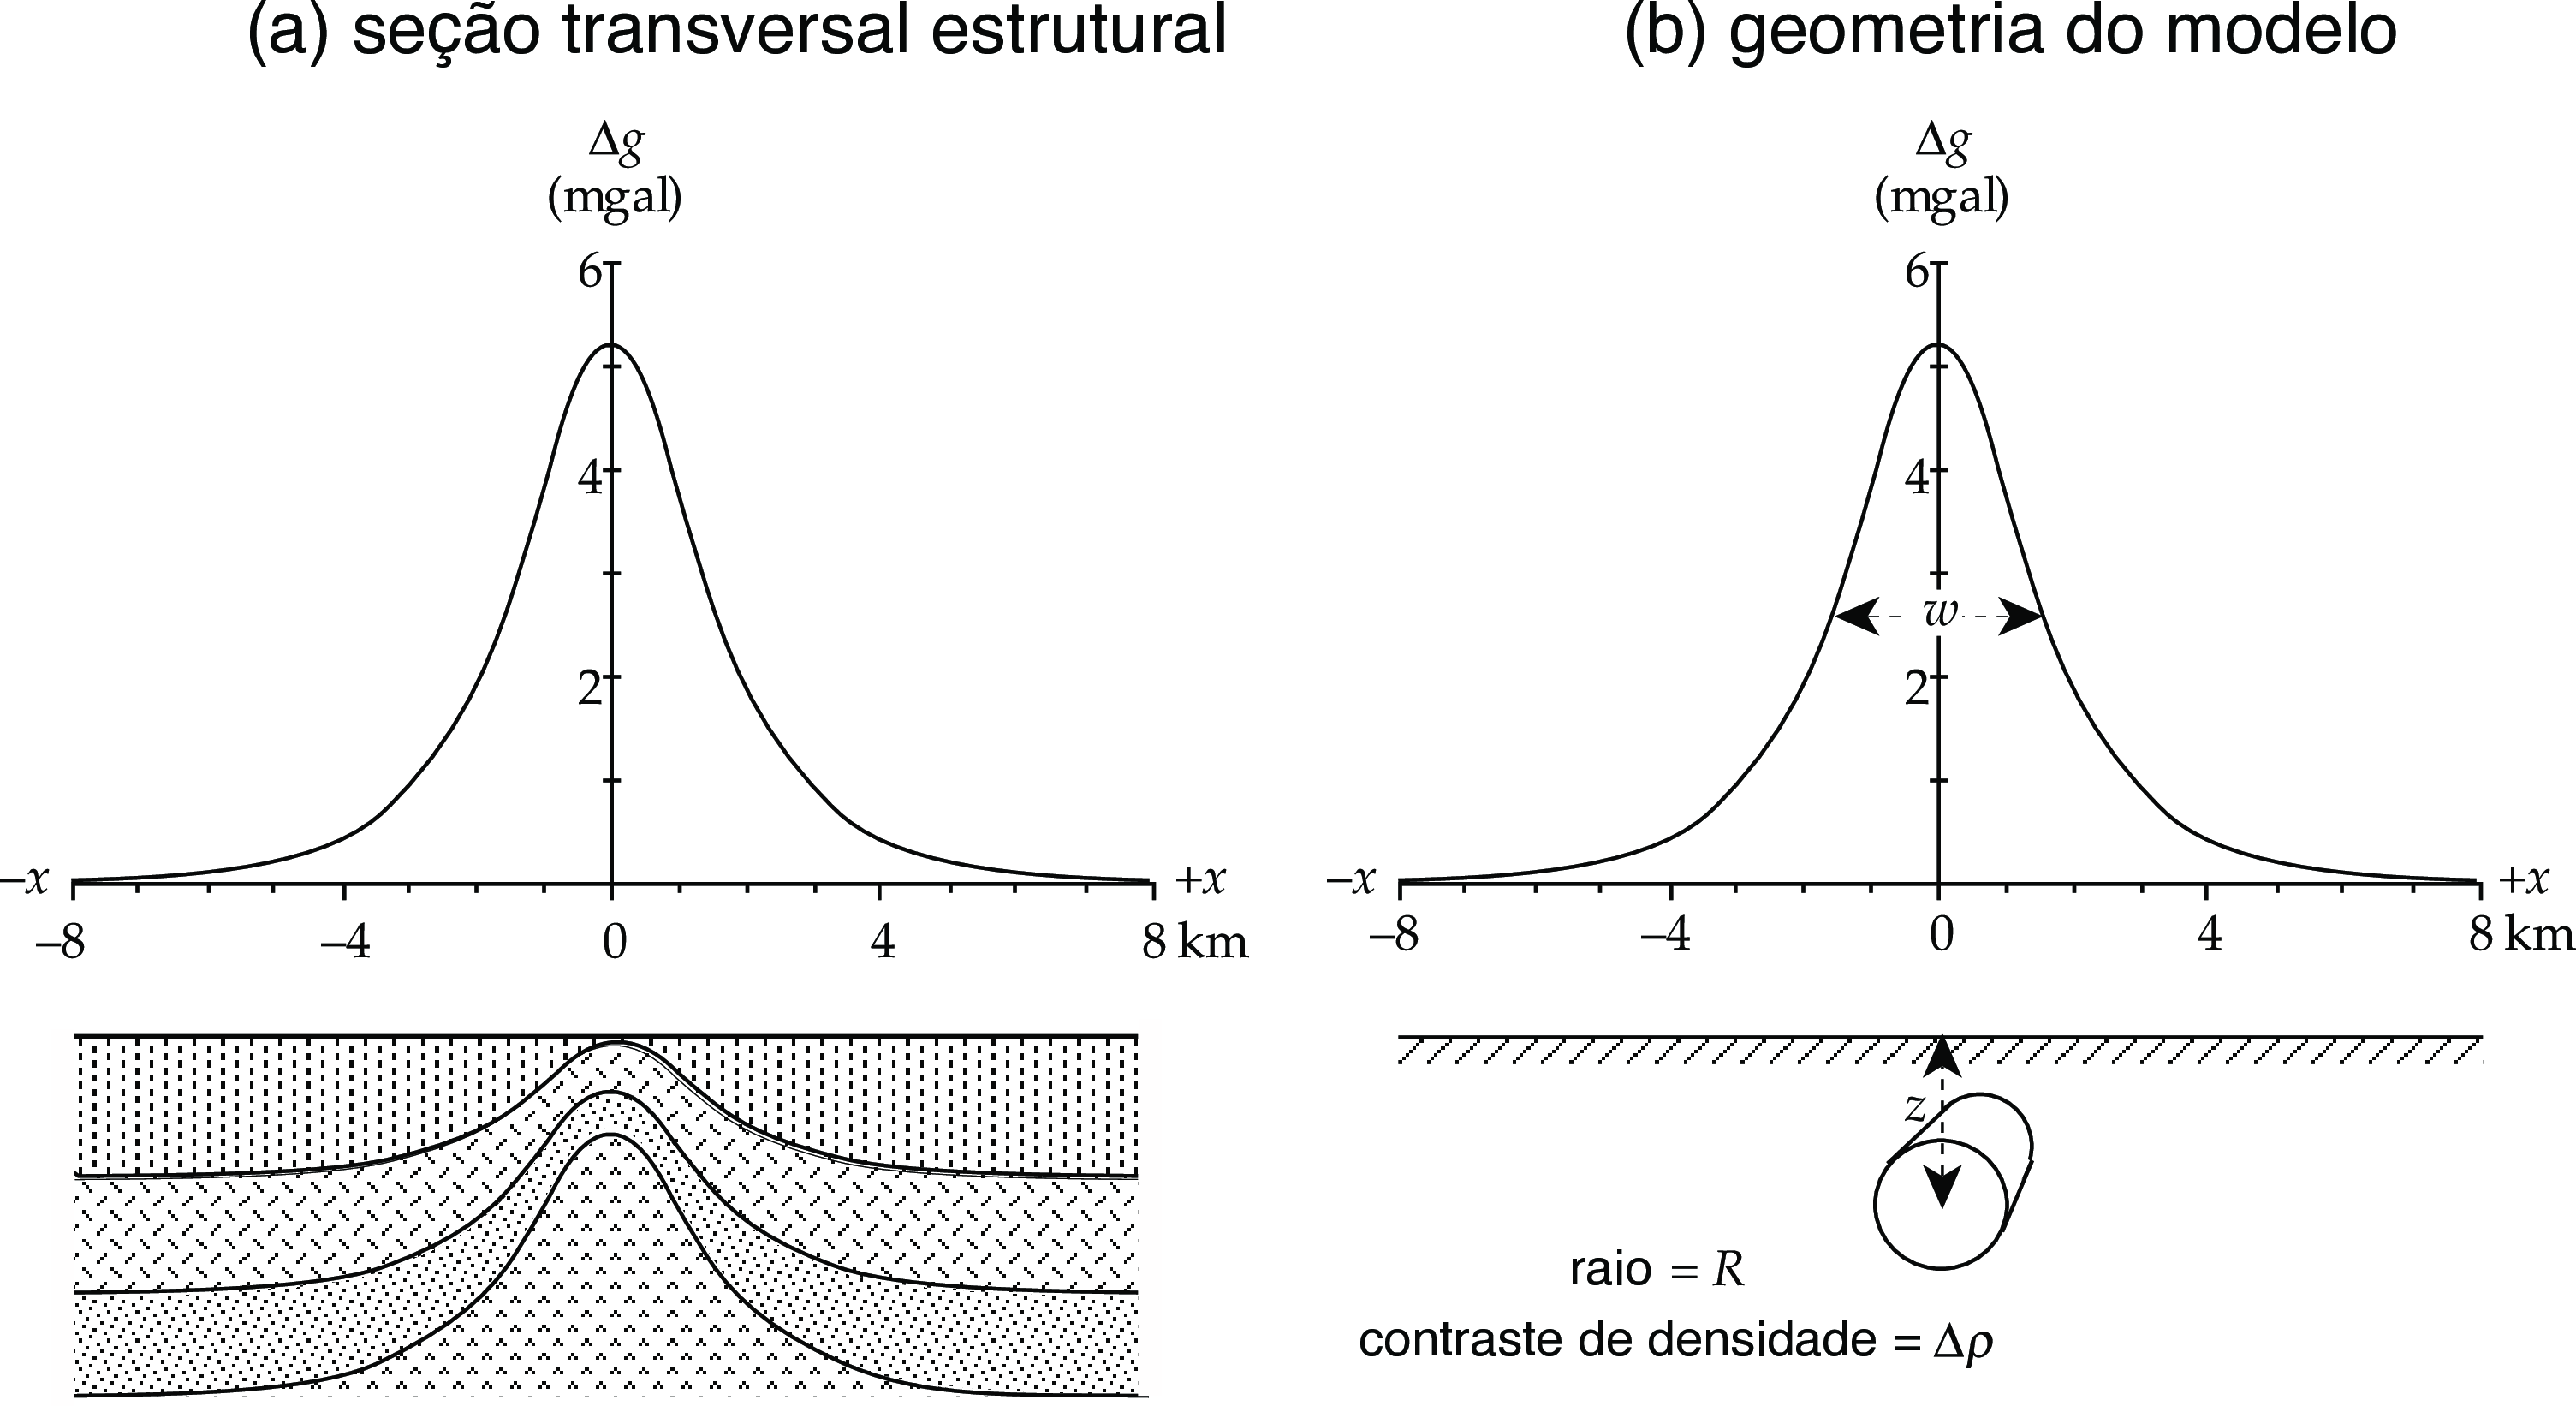
\includegraphics[width=0.8\linewidth]{fig/Fig_02.44} 

}

\caption{Cálculo da anomalia gravitacional de um anticlinal: (a) seção transversal estrutural, (b) geometria do modelo por um cilindro infinito.}\label{fig:cilindro1}
\end{figure}

Um cilindro horizontal pode ser considerado como composto de numerosos elementos de linha paralelos ao seu eixo. A área da seção transversal de um elemento (Figura \ref{fig:cilindro2}) fornece uma anomalia de massa por unidade de comprimento, \(m=\Delta\rho\, r\,dr\, d\theta\). A contribuição \(d\Psi\) de um elemento de linha para o potencial na superfície é

\begin{figure}

{\centering 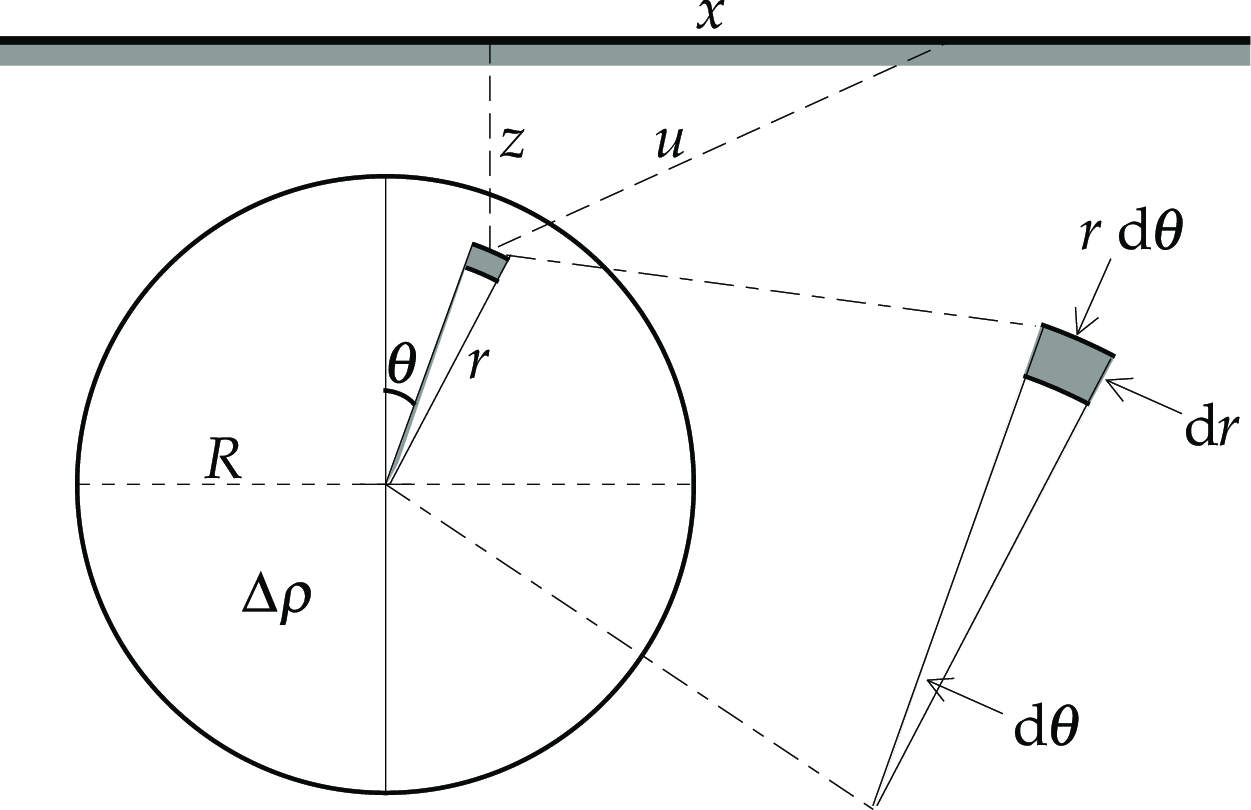
\includegraphics[width=0.6\linewidth]{fig/Fig_02.45} 

}

\caption{Geometria da seção transversal para o cálculo da anomalia gravitacional de um cilindro horizontal enterrado feito de elementos de linhas paralelos ao seu eixo.}\label{fig:cilindro2}
\end{figure}

\begin{equation}
\mathrm{d} \Psi=2 G \Delta \rho \log _{\mathrm{e}}\left(\frac{1}{u}\right) r \mathrm{d} r \mathrm{d} \theta \label{eq:0261}
\end{equation}

A integração sobre a seção transversal do cilindro dá o seu potencial \(\Psi\); a anomalia gravitacional vertical do cilindro é então encontrada diferenciando-se \(\Psi\) em relação a \(z\). Observando que \(du/dz=z/u\) conseguimos

\begin{equation}
\begin{aligned} \Delta g_{z} &=-\frac{\partial \Psi}{\partial z}=-\frac{z}{u} \frac{\partial \Psi}{\partial u} \\ &=-\frac{2 G \Delta \rho}{u} \int_{0}^{2 \pi} \int_{0}^{R} \frac{\partial}{\partial u} \log _{\mathrm{e}}\left(\frac{1}{u}\right) r \mathrm{d} r \mathrm{d} \theta \end{aligned} \label{eq:0262}
\end{equation}

Depois de realizar a diferenciação dentro da integral, isso simplifica

\begin{equation}
\Delta g_{z}=\frac{2 G \Delta \rho z}{u^{2}} \int_{0}^{2 \pi} \int_{0}^{R} r \mathrm{d} r \mathrm{d} \theta=\frac{2 \pi G R^{2} \Delta \rho z}{x^{2}+z^{2}} \label{eq:0263}
\end{equation}

Comparando as equações \eqref{eq:0263} e \eqref{eq:0258} é evidente que a anomalia gravitacional do cilindro é a mesma que a de um elemento de massa linear concentrado ao longo de seu eixo, com massa \(m=\pi R^2\Delta\rho\) por unidade de comprimento ao longo da direção da estrutura. A anomalia pode ser escrita

\begin{equation}
\Delta g_{z}=2 \pi G\left(\frac{\Delta \rho R^{2}}{z}\right)\left[\frac{1}{1+(x / z)^{2}}\right]  \label{eq:0264}
\end{equation}

A forma da anomalia em um perfil normal a estrutura (Figura \ref{fig:cilindro1}b) assemelha-se à de uma esfera (Figura \ref{fig:esferas}). O valor central do pico \(\Delta g_0\) é dado por

\begin{equation}
\Delta g_{0}=2 \pi G\left(\frac{\Delta \rho R^{2}}{z}\right)  \label{eq:0265}
\end{equation}

A anomalia de um cilindro horizontal diminui lateralmente menos rapidamente que a de uma esfera, devido à longa extensão do cilindro normal ao perfil. A ``largura de meia altura'' da anomalia depende novamente da profundidade \(z\) do eixo do cilindro; Neste caso, a profundidade é dada por \(z=0.5w\).

\hypertarget{fina-camada-horizontal}{%
\paragraph{Fina camada horizontal}\label{fina-camada-horizontal}}

Agora, calculamos a anomalia de uma fina camada horizontal de comprimento infinito normal ao plano do perfil. Isto é feito substituindo de modo fictício a camada por numerosos elementos de linha infinitamente longos colocados lado a lado. Seja a profundidade da camada ser \(z\), sua espessura \(t\) e seu contraste de densidade \(\Delta\rho\) (Figura \ref{fig:folha}a); a massa por unidade de comprimento na direção \(y\) de um elemento de linha de largura \(dx\) é \((\Delta \rho t dx)\). Substituindo na Equação \eqref{eq:0258} fornece a anomalia gravitacional do elemento de linha; a anomalia da fina camada é então computada pela integração entre os limites \(x_1\) e \(x_2\) (Figura \ref{fig:folha}b)

\begin{figure}

{\centering 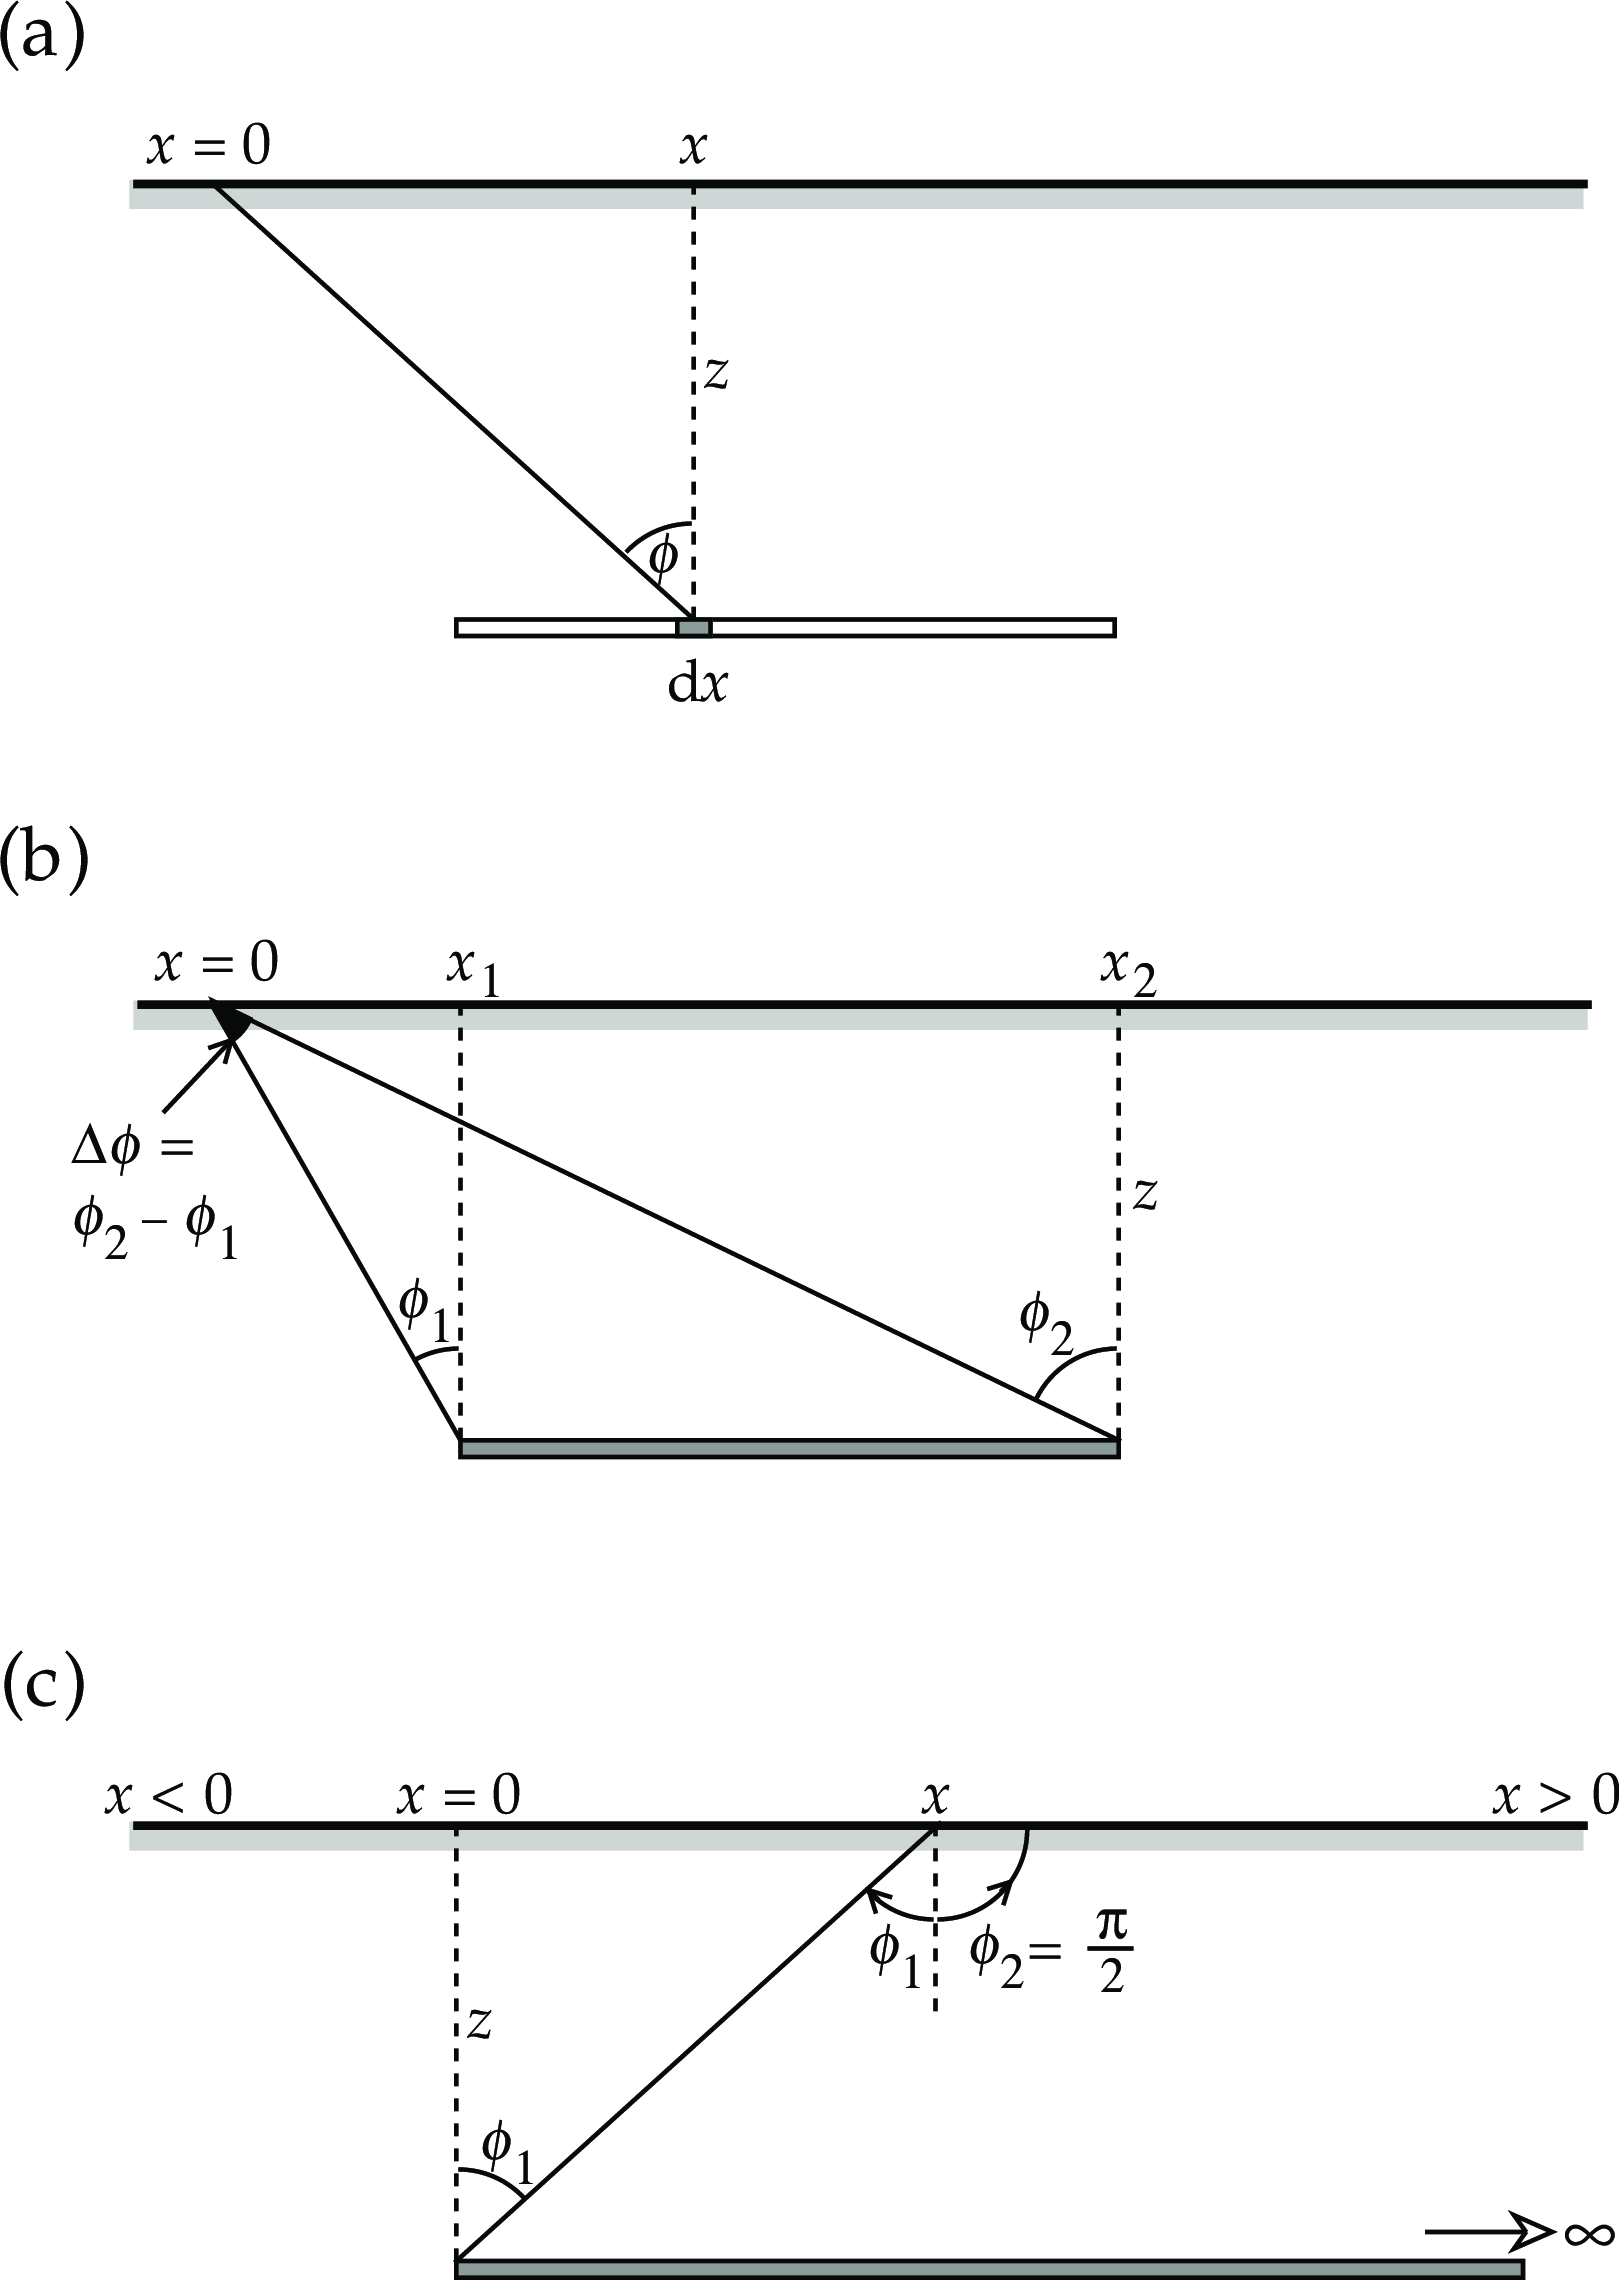
\includegraphics[width=0.6\linewidth]{fig/Fig_02.46} 

}

\caption{Geometria para cálculo da anomalia gravimétrica através de uma fina camada horizontal: (a) subdivisão da faixa em elementos de linha de largura $dx$, (b) fina faixa entre os limites horizontais $x_1$ e $x_2$ e (c) fina camada horizontal semi-infinita.}\label{fig:folha}
\end{figure}

\begin{equation}
\begin{aligned} \Delta g_{z} &=2 G \Delta \rho t z \int_{x_{1}}^{x_{2}} \frac{\mathrm{d} x}{x^{2}+z^{2}} \\ &=2 G \Delta \rho t\left[\tan ^{-1}\left(\frac{x_{2}}{z}\right)-\tan ^{-1}\left(\frac{x_{1}}{z}\right)\right]. \end{aligned}  \label{eq:0267}
\end{equation}

Escrevendo \(\tan ^{-1}\left(x_{1} / z\right)=\phi_{1}\) e \(\tan ^{-1}\left(x_{2} / z\right)=\phi_{2}\) como na (Figura \ref{fig:folha}c) equação torna-se

\begin{equation}
\Delta g_{z}=2 G \Delta \rho t\left[\phi_{2}-\phi_{1}\right] \label{eq:0268}
\end{equation}

isto é, a anomalia gravitacional da fita horizontal é proporcional ao ângulo que ela subtende no ponto de medição.

A anomalia de uma folha horizontal semi-infinita é um caso limitante desse resultado. Para referência mais fácil, a origem de \(x\) é movida para a borda da folha, de modo que as distâncias para a esquerda são negativas e as da direita são positivas (Figura \ref{fig:folha}c). Isso faz \(\phi_{1}=-\tan ^{-1}(x / z)\). A extremidade remota da folha está no infinito e \(\phi_2 =\pi / 2\). A anomalia da gravidade é então

\begin{equation}
\Delta g_{z}=2 G \Delta \rho t\left[\frac{\pi}{2}+\tan ^{-1}\left(\frac{x}{z}\right)\right]  \label{eq:0269}
\end{equation}

Um outro exemplo é a folha horizontal infinita, que se estende ao infinito nas direções positiva e negativa \(x\) e \(y\). Com \(\phi_2=\pi/2\) e \(\phi_1=-\pi/2\) a anomalia é

\begin{equation}
\Delta g_{z}=2 \pi G \Delta \rho t \label{eq:0270}
\end{equation}

que é a mesma expressão para a correção da placa Bouguer.

\hypertarget{calha-horizontal-modelo-para-uma-falha-vertical}{%
\subsubsection{Calha horizontal: modelo para uma falha vertical}\label{calha-horizontal-modelo-para-uma-falha-vertical}}

A anomalia gravitacional através de uma falha vertical aumenta progressivamente para um valor máximo sobre o lado elevado (Figura \ref{fig:slab}a). Isso é interpretado devido ao deslocamento ascendente do material mais denso, que causa um contraste de densidade horizontal ao longo de um degrau vertical de altura \(h\) (Figura \ref{fig:slab}b). O bloco com falha pode ser modelado como uma calha horizontal semi-infinita de altura \(h\) e contraste de densidade \(\Delta\rho\) com seu ponto médio na profundidade \(z_0\) (Figura \ref{fig:slab}c).

\begin{figure}

{\centering 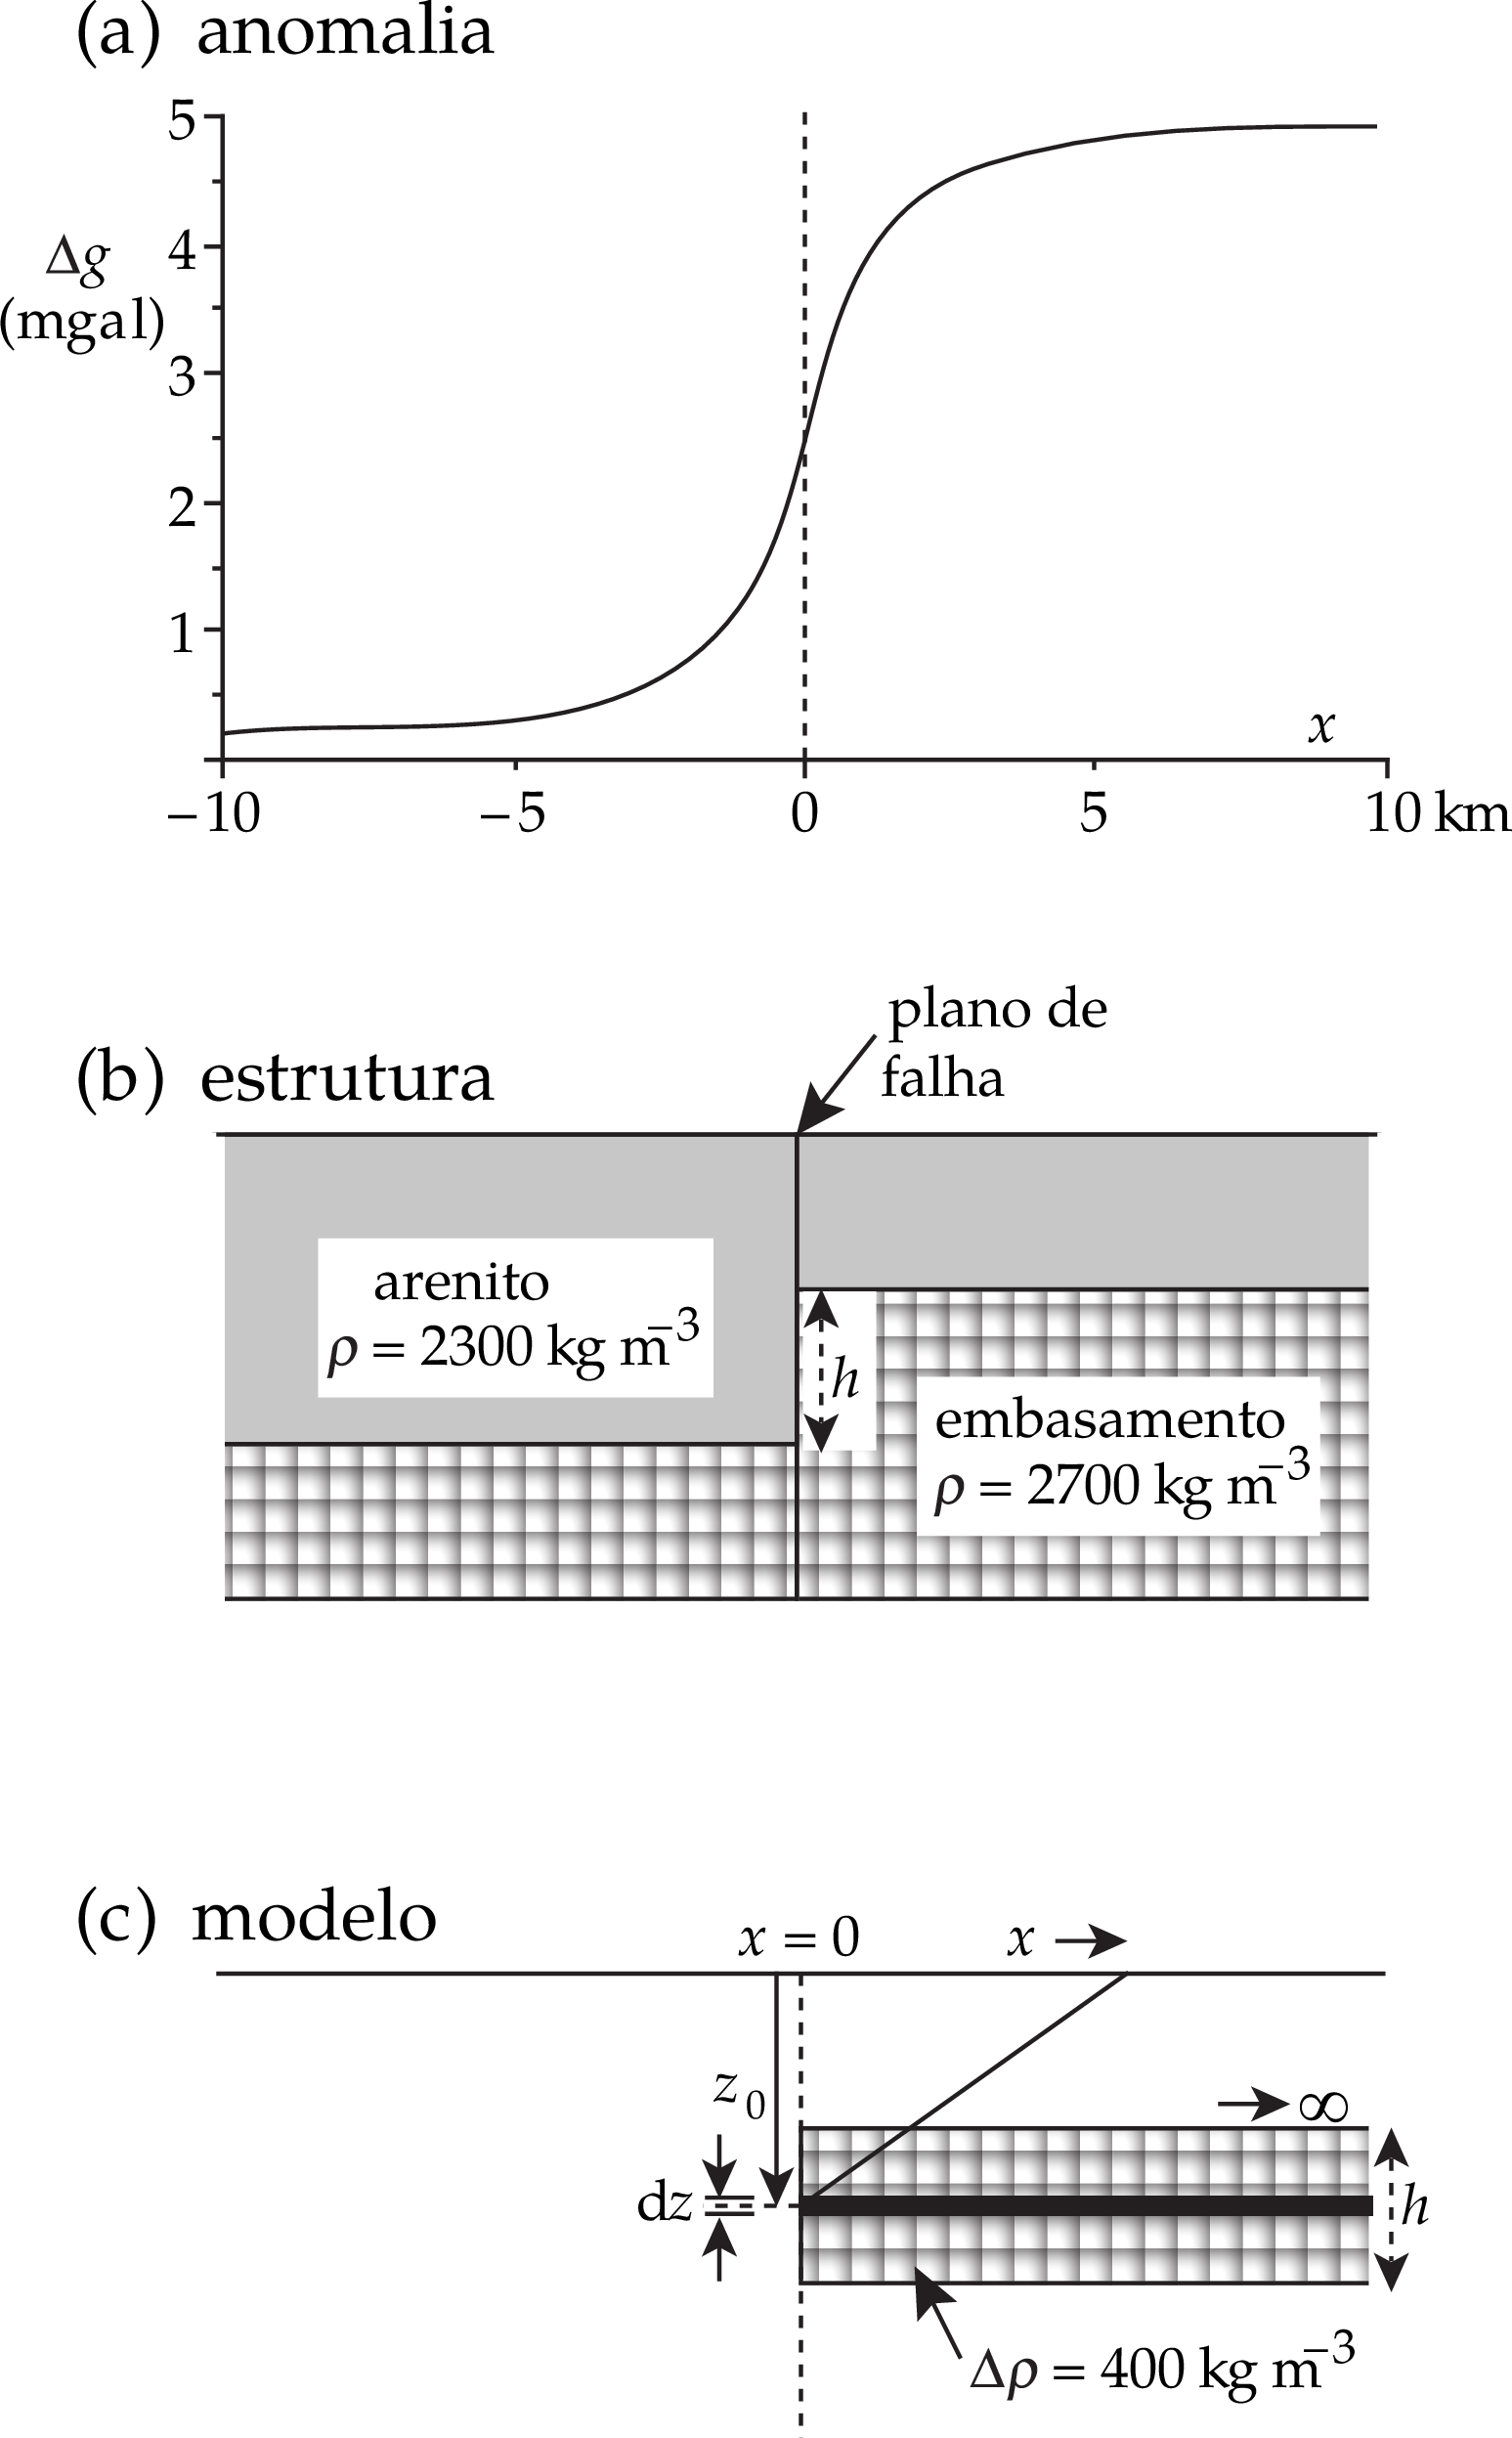
\includegraphics[width=0.6\linewidth]{fig/Fig_02.47} 

}

\caption{(a) A anomalia da gravidade através de uma falha vertical; (b) estrutura de uma falha com deslocamento vertical $h$, e (c) modelo do corpo anômalo como uma calha horizontal semi-infinita de altura $h$.}\label{fig:slab}
\end{figure}

Considere a calha ser dividida em finas folhas semi-infinitas horizontais de espessura \(d\)z na profundidade \(z\). A anomalia gravitacional de uma dada folha é dada pela Equação \eqref{eq:0269} com \(dz\) para a espessura \(t\). A anomalia da calha semi-infinita é encontrada pela integração em relação a \(z\) sobre a espessura da calha; os limites de integração são \(z-(h/2)\) e \(z+(h/2)\). Depois de termos ligeiramente rearranjados isso dá

\begin{equation}
\Delta g_{z}=2 G \Delta \rho h\left[\frac{\pi}{2}+\frac{1}{h}\int_{z_{0}-h / 2}^{z_{0}+h / 2} \tan ^{-1}\left(\frac{x}{z}\right) \mathrm{d} z\right] \label{eq:0271}
\end{equation}

A segunda expressão entre parênteses é o valor médio do ângulo \(\tan ^{-1}(x / z)\) em média sobre a altura do degrau de falha. Isso pode ser substituído por uma boa aproximação pelo valor no ponto médio da degrau, na profundidade \(z_0\). Isto dá

\begin{equation}
\Delta g_{z}=2 G \Delta \rho h\left[\frac{\pi}{2}+\tan ^{-1}\left(\frac{x}{z_{0}}\right)\right] \label{eq:0272}
\end{equation}

Comparação desta expressão com a Equação \eqref{eq:0269} mostra que a anomalia da falha vertical (ou uma calha horizontal semi-infinita) é a mesma que se a calha anômala fosse substituída por uma fina camada de espessura \(h\) no ponto médio do degrau vertical. A equação \eqref{eq:0272} é chamada de ``aproximação de fina folha''. Ela é precisa em cerca de \(2\%\) desde que \(z_0>2h\).

\hypertarget{exercicios}{%
\section{Exercícios}\label{exercicios}}

\BeginKnitrBlock{exercise}
\protect\hypertarget{exr:exr1}{}{\label{exr:exr1} } Descreva o princípio de funcionamento de um gravímetro.
\EndKnitrBlock{exercise}

\BeginKnitrBlock{exercise}
\protect\hypertarget{exr:exr2}{}{\label{exr:exr2} }Explique por que um gravímetro só fornece medidas relativas de gravidade.
\EndKnitrBlock{exercise}

\BeginKnitrBlock{exercise}
\protect\hypertarget{exr:exr3}{}{\label{exr:exr3} }O que é o geoide? O que é elipsoide de referência? Como e por que eles diferem?
\EndKnitrBlock{exercise}

\BeginKnitrBlock{exercise}
\protect\hypertarget{exr:exr4}{}{\label{exr:exr4} } O que é uma anomalia geoidal? Explique como um positivo (ou negativa) surge a anomalia.
\EndKnitrBlock{exercise}

\BeginKnitrBlock{exercise}
\protect\hypertarget{exr:exr5}{}{\label{exr:exr5} }O que é gravidade normal? O que a palavra normal implica? Qual superfície está envolvida?
\EndKnitrBlock{exercise}

\BeginKnitrBlock{exercise}
\protect\hypertarget{exr:exr6}{}{\label{exr:exr6} }A aceleração gravitacional é direcionada para um centro de massa. Com a ajuda de um esboço que mostra que as direções das componentes da gravidade, explique por que a gravidade não é uma aceleração dirigida centralmente.
\EndKnitrBlock{exercise}

\BeginKnitrBlock{exercise}
\protect\hypertarget{exr:exr7}{}{\label{exr:exr7} }Anote a expressão geral para a fórmula normal de gravidade. Explique o que determinam os parâmetros geofísicos em cada uma das constantes na fórmula?
\EndKnitrBlock{exercise}

\BeginKnitrBlock{exercise}
\protect\hypertarget{exr:exr8}{}{\label{exr:exr8} }O que é a correção topográfica na redução de dados de gravidade? Por que isso é necessário?
\EndKnitrBlock{exercise}

\bibliography{book.bib}


\end{document}
